\documentclass[twoside]{book}

% Packages required by doxygen
\usepackage{fixltx2e}
\usepackage{calc}
\usepackage{doxygen}
\usepackage[export]{adjustbox} % also loads graphicx
\usepackage{graphicx}
\usepackage[utf8]{inputenc}
\usepackage{makeidx}
\usepackage{multicol}
\usepackage{multirow}
\PassOptionsToPackage{warn}{textcomp}
\usepackage{textcomp}
\usepackage[nointegrals]{wasysym}
\usepackage[table]{xcolor}

% Font selection
\usepackage[T1]{fontenc}
\usepackage[scaled=.90]{helvet}
\usepackage{courier}
\usepackage{amssymb}
\usepackage{sectsty}
\renewcommand{\familydefault}{\sfdefault}
\allsectionsfont{%
  \fontseries{bc}\selectfont%
  \color{darkgray}%
}
\renewcommand{\DoxyLabelFont}{%
  \fontseries{bc}\selectfont%
  \color{darkgray}%
}
\newcommand{\+}{\discretionary{\mbox{\scriptsize$\hookleftarrow$}}{}{}}

% Page & text layout
\usepackage{geometry}
\geometry{%
  a4paper,%
  top=2.5cm,%
  bottom=2.5cm,%
  left=2.5cm,%
  right=2.5cm%
}
\tolerance=750
\hfuzz=15pt
\hbadness=750
\setlength{\emergencystretch}{15pt}
\setlength{\parindent}{0cm}
\setlength{\parskip}{3ex plus 2ex minus 2ex}
\makeatletter
\renewcommand{\paragraph}{%
  \@startsection{paragraph}{4}{0ex}{-1.0ex}{1.0ex}{%
    \normalfont\normalsize\bfseries\SS@parafont%
  }%
}
\renewcommand{\subparagraph}{%
  \@startsection{subparagraph}{5}{0ex}{-1.0ex}{1.0ex}{%
    \normalfont\normalsize\bfseries\SS@subparafont%
  }%
}
\makeatother

% Headers & footers
\usepackage{fancyhdr}
\pagestyle{fancyplain}
\fancyhead[LE]{\fancyplain{}{\bfseries\thepage}}
\fancyhead[CE]{\fancyplain{}{}}
\fancyhead[RE]{\fancyplain{}{\bfseries\leftmark}}
\fancyhead[LO]{\fancyplain{}{\bfseries\rightmark}}
\fancyhead[CO]{\fancyplain{}{}}
\fancyhead[RO]{\fancyplain{}{\bfseries\thepage}}
\fancyfoot[LE]{\fancyplain{}{}}
\fancyfoot[CE]{\fancyplain{}{}}
\fancyfoot[RE]{\fancyplain{}{\bfseries\scriptsize Generated by Doxygen }}
\fancyfoot[LO]{\fancyplain{}{\bfseries\scriptsize Generated by Doxygen }}
\fancyfoot[CO]{\fancyplain{}{}}
\fancyfoot[RO]{\fancyplain{}{}}
\renewcommand{\footrulewidth}{0.4pt}
\renewcommand{\chaptermark}[1]{%
  \markboth{#1}{}%
}
\renewcommand{\sectionmark}[1]{%
  \markright{\thesection\ #1}%
}

% Indices & bibliography
\usepackage{natbib}
\usepackage[titles]{tocloft}
\setcounter{tocdepth}{3}
\setcounter{secnumdepth}{5}
\makeindex

% Hyperlinks (required, but should be loaded last)
\usepackage{ifpdf}
\ifpdf
  \usepackage[pdftex,pagebackref=true]{hyperref}
\else
  \usepackage[ps2pdf,pagebackref=true]{hyperref}
\fi
\hypersetup{%
  colorlinks=true,%
  linkcolor=blue,%
  citecolor=blue,%
  unicode%
}

% Custom commands
\newcommand{\clearemptydoublepage}{%
  \newpage{\pagestyle{empty}\cleardoublepage}%
}

\usepackage{caption}
\captionsetup{labelsep=space,justification=centering,font={bf},singlelinecheck=off,skip=4pt,position=top}

%===== C O N T E N T S =====

\begin{document}

% Titlepage & ToC
\hypersetup{pageanchor=false,
             bookmarksnumbered=true,
             pdfencoding=unicode
            }
\pagenumbering{alph}
\begin{titlepage}
\vspace*{7cm}
\begin{center}%
{\Large R\+ET Alban }\\
\vspace*{1cm}
{\large Generated by Doxygen 1.8.13}\\
\end{center}
\end{titlepage}
\clearemptydoublepage
\pagenumbering{roman}
\tableofcontents
\clearemptydoublepage
\pagenumbering{arabic}
\hypersetup{pageanchor=true}

%--- Begin generated contents ---
\chapter{R\+ET Project Alban}
\label{index}\hypertarget{index}{}\hypertarget{index_description_main}{}\section{Description}\label{index_description_main}
The application you run for the R\+ET to communicate with the Rpi. The movement of the robot, the end effector cartesian position, the information about the button are the input of this function The output of the application is to know if the button are pressed inside an interval of time The interval of time is defined as the time the end effector enter and live the button\textquotesingle{}s area\hypertarget{index_notes_main}{}\section{Notes}\label{index_notes_main}
Copyright (c) 2021 Alban Boytard. All rights reserved. 
\chapter{Namespace Index}
\section{Packages}
Here are the packages with brief descriptions (if available)\+:\begin{DoxyCompactList}
\item\contentsline{section}{\hyperlink{namespaceButton__Masher__Application__Output}{Button\+\_\+\+Masher\+\_\+\+Application\+\_\+\+Output} }{\pageref{namespaceButton__Masher__Application__Output}}{}
\item\contentsline{section}{\hyperlink{namespaceRET__config}{R\+E\+T\+\_\+config} }{\pageref{namespaceRET__config}}{}
\item\contentsline{section}{\hyperlink{namespaceRET__data__processing}{R\+E\+T\+\_\+data\+\_\+processing} }{\pageref{namespaceRET__data__processing}}{}
\item\contentsline{section}{\hyperlink{namespaceRET__main}{R\+E\+T\+\_\+main} }{\pageref{namespaceRET__main}}{}
\item\contentsline{section}{\hyperlink{namespaceRET__Parameter}{R\+E\+T\+\_\+\+Parameter} }{\pageref{namespaceRET__Parameter}}{}
\item\contentsline{section}{\hyperlink{namespaceRET__socket}{R\+E\+T\+\_\+socket} }{\pageref{namespaceRET__socket}}{}
\end{DoxyCompactList}

\chapter{Hierarchical Index}
\section{Class Hierarchy}
This inheritance list is sorted roughly, but not completely, alphabetically\+:\begin{DoxyCompactList}
\item \contentsline{section}{Btn}{\pageref{classRET__config_1_1Btn}}{}
\begin{DoxyCompactList}
\item \contentsline{section}{Btn\+\_\+area}{\pageref{classRET__config_1_1Btn__area}}{}
\end{DoxyCompactList}
\item \contentsline{section}{Button\+\_\+\+Masher\+\_\+\+Application\+\_\+node\+\_\+listener}{\pageref{classButton__Masher__Application__Output_1_1Button__Masher__Application__node__listener}}{}
\begin{DoxyCompactList}
\item \contentsline{section}{R\+E\+T\+\_\+\+Parameter}{\pageref{classRET__Parameter_1_1RET__Parameter}}{}
\begin{DoxyCompactList}
\item \contentsline{section}{R\+E\+T\+\_\+data\+\_\+processing}{\pageref{classRET__data__processing_1_1RET__data__processing}}{}
\item \contentsline{section}{Computer\+\_\+\+Receive\+Message\+\_\+\+Rpi}{\pageref{classRET__socket_1_1Computer__ReceiveMessage__Rpi}}{}
\item \contentsline{section}{Computer\+\_\+\+Send\+Message\+\_\+\+Rpi}{\pageref{classRET__socket_1_1Computer__SendMessage__Rpi}}{}
\item \contentsline{section}{Computer\+\_\+\+Socket\+Client\+\_\+\+R\+ET}{\pageref{classRET__socket_1_1Computer__SocketClient__RET}}{}
\end{DoxyCompactList}
\end{DoxyCompactList}
\item Thread\begin{DoxyCompactList}
\item \contentsline{section}{R\+E\+T\+\_\+data\+\_\+processing}{\pageref{classRET__data__processing_1_1RET__data__processing}}{}
\item \contentsline{section}{Computer\+\_\+\+Receive\+Message\+\_\+\+Rpi}{\pageref{classRET__socket_1_1Computer__ReceiveMessage__Rpi}}{}
\item \contentsline{section}{Computer\+\_\+\+Send\+Message\+\_\+\+Rpi}{\pageref{classRET__socket_1_1Computer__SendMessage__Rpi}}{}
\end{DoxyCompactList}
\end{DoxyCompactList}

\chapter{Class Index}
\section{Class List}
Here are the classes, structs, unions and interfaces with brief descriptions\+:\begin{DoxyCompactList}
\item\contentsline{section}{\hyperlink{classRET__config_1_1Btn}{Btn} \\*The \hyperlink{classRET__config_1_1Btn}{Btn} base class }{\pageref{classRET__config_1_1Btn}}{}
\item\contentsline{section}{\hyperlink{classRET__config_1_1Btn__area}{Btn\+\_\+area} \\*The \hyperlink{classRET__config_1_1Btn__area}{Btn\+\_\+area} class }{\pageref{classRET__config_1_1Btn__area}}{}
\item\contentsline{section}{\hyperlink{classButton__Masher__Application__Output_1_1Button__Masher__Application__node__listener}{Button\+\_\+\+Masher\+\_\+\+Application\+\_\+node\+\_\+listener} \\*The \hyperlink{classButton__Masher__Application__Output_1_1Button__Masher__Application__node__listener}{Button\+\_\+\+Masher\+\_\+\+Application\+\_\+node\+\_\+listener} base class }{\pageref{classButton__Masher__Application__Output_1_1Button__Masher__Application__node__listener}}{}
\item\contentsline{section}{\hyperlink{classRET__socket_1_1Computer__ReceiveMessage__Rpi}{Computer\+\_\+\+Receive\+Message\+\_\+\+Rpi} \\*The \hyperlink{classRET__socket_1_1Computer__ReceiveMessage__Rpi}{Computer\+\_\+\+Receive\+Message\+\_\+\+Rpi} R\+ET class }{\pageref{classRET__socket_1_1Computer__ReceiveMessage__Rpi}}{}
\item\contentsline{section}{\hyperlink{classRET__socket_1_1Computer__SendMessage__Rpi}{Computer\+\_\+\+Send\+Message\+\_\+\+Rpi} \\*The \hyperlink{classRET__socket_1_1Computer__SendMessage__Rpi}{Computer\+\_\+\+Send\+Message\+\_\+\+Rpi} R\+ET class }{\pageref{classRET__socket_1_1Computer__SendMessage__Rpi}}{}
\item\contentsline{section}{\hyperlink{classRET__socket_1_1Computer__SocketClient__RET}{Computer\+\_\+\+Socket\+Client\+\_\+\+R\+ET} \\*The \hyperlink{classRET__socket_1_1Computer__SocketClient__RET}{Computer\+\_\+\+Socket\+Client\+\_\+\+R\+ET} R\+ET class }{\pageref{classRET__socket_1_1Computer__SocketClient__RET}}{}
\item\contentsline{section}{\hyperlink{classRET__data__processing_1_1RET__data__processing}{R\+E\+T\+\_\+data\+\_\+processing} \\*The \hyperlink{classRET__data__processing_1_1RET__data__processing}{R\+E\+T\+\_\+data\+\_\+processing} class }{\pageref{classRET__data__processing_1_1RET__data__processing}}{}
\item\contentsline{section}{\hyperlink{classRET__Parameter_1_1RET__Parameter}{R\+E\+T\+\_\+\+Parameter} \\*The input of this function is the cartesian position of the end effector given by another node!!!!!!!!!!!!!!! }{\pageref{classRET__Parameter_1_1RET__Parameter}}{}
\end{DoxyCompactList}

\chapter{File Index}
\section{File List}
Here is a list of all files with brief descriptions\+:\begin{DoxyCompactList}
\item\contentsline{section}{/home/ret/workspaces/ret/src/ret/scripts/\hyperlink{Button__Masher__Application__Output_8py}{Button\+\_\+\+Masher\+\_\+\+Application\+\_\+\+Output.\+py} }{\pageref{Button__Masher__Application__Output_8py}}{}
\item\contentsline{section}{/home/ret/workspaces/ret/src/ret/scripts/\hyperlink{RET__config_8py}{R\+E\+T\+\_\+config.\+py} }{\pageref{RET__config_8py}}{}
\item\contentsline{section}{/home/ret/workspaces/ret/src/ret/scripts/\hyperlink{RET__data__processing_8py}{R\+E\+T\+\_\+data\+\_\+processing.\+py} }{\pageref{RET__data__processing_8py}}{}
\item\contentsline{section}{/home/ret/workspaces/ret/src/ret/scripts/\hyperlink{RET__main_8py}{R\+E\+T\+\_\+main.\+py} }{\pageref{RET__main_8py}}{}
\item\contentsline{section}{/home/ret/workspaces/ret/src/ret/scripts/\hyperlink{RET__Parameter_8py}{R\+E\+T\+\_\+\+Parameter.\+py} }{\pageref{RET__Parameter_8py}}{}
\item\contentsline{section}{/home/ret/workspaces/ret/src/ret/scripts/\hyperlink{RET__socket_8py}{R\+E\+T\+\_\+socket.\+py} }{\pageref{RET__socket_8py}}{}
\end{DoxyCompactList}

\chapter{Namespace Documentation}
\hypertarget{namespaceButton__Masher__Application__Output}{}\section{Button\+\_\+\+Masher\+\_\+\+Application\+\_\+\+Output Namespace Reference}
\label{namespaceButton__Masher__Application__Output}\index{Button\+\_\+\+Masher\+\_\+\+Application\+\_\+\+Output@{Button\+\_\+\+Masher\+\_\+\+Application\+\_\+\+Output}}
\subsection*{Classes}
\begin{DoxyCompactItemize}
\item 
class \hyperlink{classButton__Masher__Application__Output_1_1Button__Masher__Application__node__listener}{Button\+\_\+\+Masher\+\_\+\+Application\+\_\+node\+\_\+listener}
\begin{DoxyCompactList}\small\item\em The \hyperlink{classButton__Masher__Application__Output_1_1Button__Masher__Application__node__listener}{Button\+\_\+\+Masher\+\_\+\+Application\+\_\+node\+\_\+listener} base class. \end{DoxyCompactList}\end{DoxyCompactItemize}
\subsection*{Functions}
\begin{DoxyCompactItemize}
\item 
def \hyperlink{namespaceButton__Masher__Application__Output_ad537c35a13781c3e28b4e3cc57ba321e}{launch\+\_\+node\+\_\+listener} ()
\begin{DoxyCompactList}\small\item\em Initialize the node tool\+\_\+pose\+\_\+publisher\+\_\+use. \end{DoxyCompactList}\end{DoxyCompactItemize}


\subsection{Function Documentation}
\mbox{\Hypertarget{namespaceButton__Masher__Application__Output_ad537c35a13781c3e28b4e3cc57ba321e}\label{namespaceButton__Masher__Application__Output_ad537c35a13781c3e28b4e3cc57ba321e}} 
\index{Button\+\_\+\+Masher\+\_\+\+Application\+\_\+\+Output@{Button\+\_\+\+Masher\+\_\+\+Application\+\_\+\+Output}!launch\+\_\+node\+\_\+listener@{launch\+\_\+node\+\_\+listener}}
\index{launch\+\_\+node\+\_\+listener@{launch\+\_\+node\+\_\+listener}!Button\+\_\+\+Masher\+\_\+\+Application\+\_\+\+Output@{Button\+\_\+\+Masher\+\_\+\+Application\+\_\+\+Output}}
\subsubsection{\texorpdfstring{launch\+\_\+node\+\_\+listener()}{launch\_node\_listener()}}
{\footnotesize\ttfamily def Button\+\_\+\+Masher\+\_\+\+Application\+\_\+\+Output.\+launch\+\_\+node\+\_\+listener (\begin{DoxyParamCaption}{ }\end{DoxyParamCaption})}



Initialize the node tool\+\_\+pose\+\_\+publisher\+\_\+use. 

\begin{DoxyReturn}{Returns}
the node tool\+\_\+pose\+\_\+publisher\+\_\+use with a high frequency spin. 

when there is a key board interrupt, kill all the node running on the computer 
\end{DoxyReturn}

\hypertarget{namespaceRET__config}{}\section{R\+E\+T\+\_\+config Namespace Reference}
\label{namespaceRET__config}\index{R\+E\+T\+\_\+config@{R\+E\+T\+\_\+config}}
\subsection*{Classes}
\begin{DoxyCompactItemize}
\item 
class \hyperlink{classRET__config_1_1Btn}{Btn}
\begin{DoxyCompactList}\small\item\em The \hyperlink{classRET__config_1_1Btn}{Btn} base class. \end{DoxyCompactList}\item 
class \hyperlink{classRET__config_1_1Btn__area}{Btn\+\_\+area}
\begin{DoxyCompactList}\small\item\em The \hyperlink{classRET__config_1_1Btn__area}{Btn\+\_\+area} class. \end{DoxyCompactList}\end{DoxyCompactItemize}
\subsection*{Variables}
\begin{DoxyCompactItemize}
\item 
float \hyperlink{namespaceRET__config_a425bc201cf7b10f0c4f1068f752e7c9b}{acceleration\+\_\+factor} = 3.\+49
\item 
\hyperlink{namespaceRET__config_af037c6b9ff0314103d8127acc9d07e0b}{Btn1} = \hyperlink{classRET__config_1_1Btn}{Btn}(\char`\"{}Btn1\char`\"{},x1,\hyperlink{namespaceRET__config_a9fe80bf4738047a31d7c162807ed85f0}{y1},\hyperlink{namespaceRET__config_a7da4886c0a2e03b8bb9ed62eb20efb78}{z1})
\item 
\hyperlink{namespaceRET__config_a118140d2896d1aff1e3c9355f9deb314}{Btn1\+\_\+area} = \hyperlink{classRET__config_1_1Btn__area}{Btn\+\_\+area}(\hyperlink{namespaceRET__config_af037c6b9ff0314103d8127acc9d07e0b}{Btn1}, \hyperlink{namespaceRET__config_abbf3fd8fafae6a457e57109bfaf9a6c5}{delta\+\_\+area}\mbox{[}0\mbox{]}, \hyperlink{namespaceRET__config_abbf3fd8fafae6a457e57109bfaf9a6c5}{delta\+\_\+area}\mbox{[}1\mbox{]}, \hyperlink{namespaceRET__config_abbf3fd8fafae6a457e57109bfaf9a6c5}{delta\+\_\+area}\mbox{[}2\mbox{]})
\item 
\hyperlink{namespaceRET__config_a73afa8c52cebd94e1889df5fbe3bec66}{Btn2} = \hyperlink{classRET__config_1_1Btn}{Btn}(\char`\"{}Btn2\char`\"{},x2,\hyperlink{namespaceRET__config_a07bcd014e69eddcf4243b2a961014eaf}{y2},\hyperlink{namespaceRET__config_a55196b87940893e540ba636218f4eb07}{z2})
\item 
\hyperlink{namespaceRET__config_a51a4083768cbc17b22a98ad63a7bf851}{Btn2\+\_\+area} = \hyperlink{classRET__config_1_1Btn__area}{Btn\+\_\+area}(\hyperlink{namespaceRET__config_a73afa8c52cebd94e1889df5fbe3bec66}{Btn2}, \hyperlink{namespaceRET__config_abbf3fd8fafae6a457e57109bfaf9a6c5}{delta\+\_\+area}\mbox{[}0\mbox{]}, \hyperlink{namespaceRET__config_abbf3fd8fafae6a457e57109bfaf9a6c5}{delta\+\_\+area}\mbox{[}1\mbox{]}, \hyperlink{namespaceRET__config_abbf3fd8fafae6a457e57109bfaf9a6c5}{delta\+\_\+area}\mbox{[}2\mbox{]})
\item 
list \hyperlink{namespaceRET__config_abbf3fd8fafae6a457e57109bfaf9a6c5}{delta\+\_\+area} = \mbox{[}0.\+06,0.\+06,0.\+01\mbox{]}
\item 
string \hyperlink{namespaceRET__config_af06655663f692a853833001d611f908d}{driver\+\_\+used} = \char`\"{}native\char`\"{}
\item 
string \hyperlink{namespaceRET__config_a6297da7d9cbabcbe91effb0271677ff3}{influxdb} = \char`\"{}R\+E\+T\+\_\+\+Test\char`\"{}
\item 
string \hyperlink{namespaceRET__config_a5ad590543d5ae7b0a89b3681d33928d8}{influxdb\+\_\+host} = \char`\"{}localhost\char`\"{}
\begin{DoxyCompactList}\small\item\em global variable for the data storage \end{DoxyCompactList}\item 
string \hyperlink{namespaceRET__config_a91cab5b28cd6867b74e2cb9f887b2948}{influxdb\+\_\+port} = \char`\"{}8086\char`\"{}
\item 
list \hyperlink{namespaceRET__config_a25b4602337319d65f44337e6ad1b0487}{list\+\_\+buttons\+\_\+area} = \mbox{[}\hyperlink{namespaceRET__config_a118140d2896d1aff1e3c9355f9deb314}{Btn1\+\_\+area},\hyperlink{namespaceRET__config_a51a4083768cbc17b22a98ad63a7bf851}{Btn2\+\_\+area}\mbox{]}
\item 
\hyperlink{namespaceRET__config_a1cc0506097479f304974f44bc5456f4a}{minimal\+\_\+time\+\_\+interval\+\_\+button\+\_\+area} = time.\+time()
\item 
bool \hyperlink{namespaceRET__config_a4132cf21a6c01ecf59141756ab5f9936}{real\+\_\+time\+\_\+processing} = True
\item 
float \hyperlink{namespaceRET__config_aff247d8ee094bb439dbb098e236455cb}{robot\+\_\+settle\+\_\+time} = 0.\+2
\begin{DoxyCompactList}\small\item\em global variable for csv logfile \end{DoxyCompactList}\item 
string \hyperlink{namespaceRET__config_a2014ea8569b3cda02e44e85f8840eba2}{socket\+\_\+host} = \textquotesingle{}10.\+4.\+11.\+117\textquotesingle{}
\begin{DoxyCompactList}\small\item\em global variable for the socket communication \end{DoxyCompactList}\item 
int \hyperlink{namespaceRET__config_a08c4648fe1aa34a4fd5ad0097d17237f}{socket\+\_\+port} = 5009
\item 
bool \hyperlink{namespaceRET__config_a94d742b756b055a53df310fd15705ede}{stop\+\_\+thread} = False
\item 
float \hyperlink{namespaceRET__config_a0fee7ae942bb4b6078c6400331aef6f1}{velocity\+\_\+factor} = 1.\+57
\item 
float \hyperlink{namespaceRET__config_a3389d8b95846602e8f94cc15f41e48e9}{x1} = -\/0.\+1
\item 
float \hyperlink{namespaceRET__config_a24d6ffb6e8780eef0c81cd97e3f4fdaf}{x2} = 0.\+05
\item 
float \hyperlink{namespaceRET__config_a9fe80bf4738047a31d7c162807ed85f0}{y1} = -\/0.\+41
\item 
float \hyperlink{namespaceRET__config_a07bcd014e69eddcf4243b2a961014eaf}{y2} = -\/0.\+41
\item 
float \hyperlink{namespaceRET__config_a7da4886c0a2e03b8bb9ed62eb20efb78}{z1} = 0.\+145
\item 
float \hyperlink{namespaceRET__config_a55196b87940893e540ba636218f4eb07}{z2} = 0.\+145
\end{DoxyCompactItemize}


\subsection{Variable Documentation}
\mbox{\Hypertarget{namespaceRET__config_a425bc201cf7b10f0c4f1068f752e7c9b}\label{namespaceRET__config_a425bc201cf7b10f0c4f1068f752e7c9b}} 
\index{R\+E\+T\+\_\+config@{R\+E\+T\+\_\+config}!acceleration\+\_\+factor@{acceleration\+\_\+factor}}
\index{acceleration\+\_\+factor@{acceleration\+\_\+factor}!R\+E\+T\+\_\+config@{R\+E\+T\+\_\+config}}
\subsubsection{\texorpdfstring{acceleration\+\_\+factor}{acceleration\_factor}}
{\footnotesize\ttfamily float acceleration\+\_\+factor = 3.\+49}

\mbox{\Hypertarget{namespaceRET__config_af037c6b9ff0314103d8127acc9d07e0b}\label{namespaceRET__config_af037c6b9ff0314103d8127acc9d07e0b}} 
\index{R\+E\+T\+\_\+config@{R\+E\+T\+\_\+config}!Btn1@{Btn1}}
\index{Btn1@{Btn1}!R\+E\+T\+\_\+config@{R\+E\+T\+\_\+config}}
\subsubsection{\texorpdfstring{Btn1}{Btn1}}
{\footnotesize\ttfamily Btn1 = \hyperlink{classRET__config_1_1Btn}{Btn}(\char`\"{}Btn1\char`\"{},x1,\hyperlink{namespaceRET__config_a9fe80bf4738047a31d7c162807ed85f0}{y1},\hyperlink{namespaceRET__config_a7da4886c0a2e03b8bb9ed62eb20efb78}{z1})}

\mbox{\Hypertarget{namespaceRET__config_a118140d2896d1aff1e3c9355f9deb314}\label{namespaceRET__config_a118140d2896d1aff1e3c9355f9deb314}} 
\index{R\+E\+T\+\_\+config@{R\+E\+T\+\_\+config}!Btn1\+\_\+area@{Btn1\+\_\+area}}
\index{Btn1\+\_\+area@{Btn1\+\_\+area}!R\+E\+T\+\_\+config@{R\+E\+T\+\_\+config}}
\subsubsection{\texorpdfstring{Btn1\+\_\+area}{Btn1\_area}}
{\footnotesize\ttfamily Btn1\+\_\+area = \hyperlink{classRET__config_1_1Btn__area}{Btn\+\_\+area}(\hyperlink{namespaceRET__config_af037c6b9ff0314103d8127acc9d07e0b}{Btn1}, \hyperlink{namespaceRET__config_abbf3fd8fafae6a457e57109bfaf9a6c5}{delta\+\_\+area}\mbox{[}0\mbox{]}, \hyperlink{namespaceRET__config_abbf3fd8fafae6a457e57109bfaf9a6c5}{delta\+\_\+area}\mbox{[}1\mbox{]}, \hyperlink{namespaceRET__config_abbf3fd8fafae6a457e57109bfaf9a6c5}{delta\+\_\+area}\mbox{[}2\mbox{]})}

\mbox{\Hypertarget{namespaceRET__config_a73afa8c52cebd94e1889df5fbe3bec66}\label{namespaceRET__config_a73afa8c52cebd94e1889df5fbe3bec66}} 
\index{R\+E\+T\+\_\+config@{R\+E\+T\+\_\+config}!Btn2@{Btn2}}
\index{Btn2@{Btn2}!R\+E\+T\+\_\+config@{R\+E\+T\+\_\+config}}
\subsubsection{\texorpdfstring{Btn2}{Btn2}}
{\footnotesize\ttfamily Btn2 = \hyperlink{classRET__config_1_1Btn}{Btn}(\char`\"{}Btn2\char`\"{},x2,\hyperlink{namespaceRET__config_a07bcd014e69eddcf4243b2a961014eaf}{y2},\hyperlink{namespaceRET__config_a55196b87940893e540ba636218f4eb07}{z2})}

\mbox{\Hypertarget{namespaceRET__config_a51a4083768cbc17b22a98ad63a7bf851}\label{namespaceRET__config_a51a4083768cbc17b22a98ad63a7bf851}} 
\index{R\+E\+T\+\_\+config@{R\+E\+T\+\_\+config}!Btn2\+\_\+area@{Btn2\+\_\+area}}
\index{Btn2\+\_\+area@{Btn2\+\_\+area}!R\+E\+T\+\_\+config@{R\+E\+T\+\_\+config}}
\subsubsection{\texorpdfstring{Btn2\+\_\+area}{Btn2\_area}}
{\footnotesize\ttfamily Btn2\+\_\+area = \hyperlink{classRET__config_1_1Btn__area}{Btn\+\_\+area}(\hyperlink{namespaceRET__config_a73afa8c52cebd94e1889df5fbe3bec66}{Btn2}, \hyperlink{namespaceRET__config_abbf3fd8fafae6a457e57109bfaf9a6c5}{delta\+\_\+area}\mbox{[}0\mbox{]}, \hyperlink{namespaceRET__config_abbf3fd8fafae6a457e57109bfaf9a6c5}{delta\+\_\+area}\mbox{[}1\mbox{]}, \hyperlink{namespaceRET__config_abbf3fd8fafae6a457e57109bfaf9a6c5}{delta\+\_\+area}\mbox{[}2\mbox{]})}

\mbox{\Hypertarget{namespaceRET__config_abbf3fd8fafae6a457e57109bfaf9a6c5}\label{namespaceRET__config_abbf3fd8fafae6a457e57109bfaf9a6c5}} 
\index{R\+E\+T\+\_\+config@{R\+E\+T\+\_\+config}!delta\+\_\+area@{delta\+\_\+area}}
\index{delta\+\_\+area@{delta\+\_\+area}!R\+E\+T\+\_\+config@{R\+E\+T\+\_\+config}}
\subsubsection{\texorpdfstring{delta\+\_\+area}{delta\_area}}
{\footnotesize\ttfamily list delta\+\_\+area = \mbox{[}0.\+06,0.\+06,0.\+01\mbox{]}}

\mbox{\Hypertarget{namespaceRET__config_af06655663f692a853833001d611f908d}\label{namespaceRET__config_af06655663f692a853833001d611f908d}} 
\index{R\+E\+T\+\_\+config@{R\+E\+T\+\_\+config}!driver\+\_\+used@{driver\+\_\+used}}
\index{driver\+\_\+used@{driver\+\_\+used}!R\+E\+T\+\_\+config@{R\+E\+T\+\_\+config}}
\subsubsection{\texorpdfstring{driver\+\_\+used}{driver\_used}}
{\footnotesize\ttfamily string driver\+\_\+used = \char`\"{}native\char`\"{}}

\mbox{\Hypertarget{namespaceRET__config_a6297da7d9cbabcbe91effb0271677ff3}\label{namespaceRET__config_a6297da7d9cbabcbe91effb0271677ff3}} 
\index{R\+E\+T\+\_\+config@{R\+E\+T\+\_\+config}!influxdb@{influxdb}}
\index{influxdb@{influxdb}!R\+E\+T\+\_\+config@{R\+E\+T\+\_\+config}}
\subsubsection{\texorpdfstring{influxdb}{influxdb}}
{\footnotesize\ttfamily string influxdb = \char`\"{}R\+E\+T\+\_\+\+Test\char`\"{}}

\mbox{\Hypertarget{namespaceRET__config_a5ad590543d5ae7b0a89b3681d33928d8}\label{namespaceRET__config_a5ad590543d5ae7b0a89b3681d33928d8}} 
\index{R\+E\+T\+\_\+config@{R\+E\+T\+\_\+config}!influxdb\+\_\+host@{influxdb\+\_\+host}}
\index{influxdb\+\_\+host@{influxdb\+\_\+host}!R\+E\+T\+\_\+config@{R\+E\+T\+\_\+config}}
\subsubsection{\texorpdfstring{influxdb\+\_\+host}{influxdb\_host}}
{\footnotesize\ttfamily string influxdb\+\_\+host = \char`\"{}localhost\char`\"{}}



global variable for the data storage 

\mbox{\Hypertarget{namespaceRET__config_a91cab5b28cd6867b74e2cb9f887b2948}\label{namespaceRET__config_a91cab5b28cd6867b74e2cb9f887b2948}} 
\index{R\+E\+T\+\_\+config@{R\+E\+T\+\_\+config}!influxdb\+\_\+port@{influxdb\+\_\+port}}
\index{influxdb\+\_\+port@{influxdb\+\_\+port}!R\+E\+T\+\_\+config@{R\+E\+T\+\_\+config}}
\subsubsection{\texorpdfstring{influxdb\+\_\+port}{influxdb\_port}}
{\footnotesize\ttfamily string influxdb\+\_\+port = \char`\"{}8086\char`\"{}}

\mbox{\Hypertarget{namespaceRET__config_a25b4602337319d65f44337e6ad1b0487}\label{namespaceRET__config_a25b4602337319d65f44337e6ad1b0487}} 
\index{R\+E\+T\+\_\+config@{R\+E\+T\+\_\+config}!list\+\_\+buttons\+\_\+area@{list\+\_\+buttons\+\_\+area}}
\index{list\+\_\+buttons\+\_\+area@{list\+\_\+buttons\+\_\+area}!R\+E\+T\+\_\+config@{R\+E\+T\+\_\+config}}
\subsubsection{\texorpdfstring{list\+\_\+buttons\+\_\+area}{list\_buttons\_area}}
{\footnotesize\ttfamily list list\+\_\+buttons\+\_\+area = \mbox{[}\hyperlink{namespaceRET__config_a118140d2896d1aff1e3c9355f9deb314}{Btn1\+\_\+area},\hyperlink{namespaceRET__config_a51a4083768cbc17b22a98ad63a7bf851}{Btn2\+\_\+area}\mbox{]}}

\mbox{\Hypertarget{namespaceRET__config_a1cc0506097479f304974f44bc5456f4a}\label{namespaceRET__config_a1cc0506097479f304974f44bc5456f4a}} 
\index{R\+E\+T\+\_\+config@{R\+E\+T\+\_\+config}!minimal\+\_\+time\+\_\+interval\+\_\+button\+\_\+area@{minimal\+\_\+time\+\_\+interval\+\_\+button\+\_\+area}}
\index{minimal\+\_\+time\+\_\+interval\+\_\+button\+\_\+area@{minimal\+\_\+time\+\_\+interval\+\_\+button\+\_\+area}!R\+E\+T\+\_\+config@{R\+E\+T\+\_\+config}}
\subsubsection{\texorpdfstring{minimal\+\_\+time\+\_\+interval\+\_\+button\+\_\+area}{minimal\_time\_interval\_button\_area}}
{\footnotesize\ttfamily minimal\+\_\+time\+\_\+interval\+\_\+button\+\_\+area = time.\+time()}

\mbox{\Hypertarget{namespaceRET__config_a4132cf21a6c01ecf59141756ab5f9936}\label{namespaceRET__config_a4132cf21a6c01ecf59141756ab5f9936}} 
\index{R\+E\+T\+\_\+config@{R\+E\+T\+\_\+config}!real\+\_\+time\+\_\+processing@{real\+\_\+time\+\_\+processing}}
\index{real\+\_\+time\+\_\+processing@{real\+\_\+time\+\_\+processing}!R\+E\+T\+\_\+config@{R\+E\+T\+\_\+config}}
\subsubsection{\texorpdfstring{real\+\_\+time\+\_\+processing}{real\_time\_processing}}
{\footnotesize\ttfamily bool real\+\_\+time\+\_\+processing = True}

\mbox{\Hypertarget{namespaceRET__config_aff247d8ee094bb439dbb098e236455cb}\label{namespaceRET__config_aff247d8ee094bb439dbb098e236455cb}} 
\index{R\+E\+T\+\_\+config@{R\+E\+T\+\_\+config}!robot\+\_\+settle\+\_\+time@{robot\+\_\+settle\+\_\+time}}
\index{robot\+\_\+settle\+\_\+time@{robot\+\_\+settle\+\_\+time}!R\+E\+T\+\_\+config@{R\+E\+T\+\_\+config}}
\subsubsection{\texorpdfstring{robot\+\_\+settle\+\_\+time}{robot\_settle\_time}}
{\footnotesize\ttfamily float robot\+\_\+settle\+\_\+time = 0.\+2}



global variable for csv logfile 

global variable to test \mbox{\Hypertarget{namespaceRET__config_a2014ea8569b3cda02e44e85f8840eba2}\label{namespaceRET__config_a2014ea8569b3cda02e44e85f8840eba2}} 
\index{R\+E\+T\+\_\+config@{R\+E\+T\+\_\+config}!socket\+\_\+host@{socket\+\_\+host}}
\index{socket\+\_\+host@{socket\+\_\+host}!R\+E\+T\+\_\+config@{R\+E\+T\+\_\+config}}
\subsubsection{\texorpdfstring{socket\+\_\+host}{socket\_host}}
{\footnotesize\ttfamily string socket\+\_\+host = \textquotesingle{}10.\+4.\+11.\+117\textquotesingle{}}



global variable for the socket communication 

\mbox{\Hypertarget{namespaceRET__config_a08c4648fe1aa34a4fd5ad0097d17237f}\label{namespaceRET__config_a08c4648fe1aa34a4fd5ad0097d17237f}} 
\index{R\+E\+T\+\_\+config@{R\+E\+T\+\_\+config}!socket\+\_\+port@{socket\+\_\+port}}
\index{socket\+\_\+port@{socket\+\_\+port}!R\+E\+T\+\_\+config@{R\+E\+T\+\_\+config}}
\subsubsection{\texorpdfstring{socket\+\_\+port}{socket\_port}}
{\footnotesize\ttfamily int socket\+\_\+port = 5009}

\mbox{\Hypertarget{namespaceRET__config_a94d742b756b055a53df310fd15705ede}\label{namespaceRET__config_a94d742b756b055a53df310fd15705ede}} 
\index{R\+E\+T\+\_\+config@{R\+E\+T\+\_\+config}!stop\+\_\+thread@{stop\+\_\+thread}}
\index{stop\+\_\+thread@{stop\+\_\+thread}!R\+E\+T\+\_\+config@{R\+E\+T\+\_\+config}}
\subsubsection{\texorpdfstring{stop\+\_\+thread}{stop\_thread}}
{\footnotesize\ttfamily bool stop\+\_\+thread = False}

\mbox{\Hypertarget{namespaceRET__config_a0fee7ae942bb4b6078c6400331aef6f1}\label{namespaceRET__config_a0fee7ae942bb4b6078c6400331aef6f1}} 
\index{R\+E\+T\+\_\+config@{R\+E\+T\+\_\+config}!velocity\+\_\+factor@{velocity\+\_\+factor}}
\index{velocity\+\_\+factor@{velocity\+\_\+factor}!R\+E\+T\+\_\+config@{R\+E\+T\+\_\+config}}
\subsubsection{\texorpdfstring{velocity\+\_\+factor}{velocity\_factor}}
{\footnotesize\ttfamily float velocity\+\_\+factor = 1.\+57}

\mbox{\Hypertarget{namespaceRET__config_a3389d8b95846602e8f94cc15f41e48e9}\label{namespaceRET__config_a3389d8b95846602e8f94cc15f41e48e9}} 
\index{R\+E\+T\+\_\+config@{R\+E\+T\+\_\+config}!x1@{x1}}
\index{x1@{x1}!R\+E\+T\+\_\+config@{R\+E\+T\+\_\+config}}
\subsubsection{\texorpdfstring{x1}{x1}}
{\footnotesize\ttfamily float x1 = -\/0.\+1}

\mbox{\Hypertarget{namespaceRET__config_a24d6ffb6e8780eef0c81cd97e3f4fdaf}\label{namespaceRET__config_a24d6ffb6e8780eef0c81cd97e3f4fdaf}} 
\index{R\+E\+T\+\_\+config@{R\+E\+T\+\_\+config}!x2@{x2}}
\index{x2@{x2}!R\+E\+T\+\_\+config@{R\+E\+T\+\_\+config}}
\subsubsection{\texorpdfstring{x2}{x2}}
{\footnotesize\ttfamily float x2 = 0.\+05}

\mbox{\Hypertarget{namespaceRET__config_a9fe80bf4738047a31d7c162807ed85f0}\label{namespaceRET__config_a9fe80bf4738047a31d7c162807ed85f0}} 
\index{R\+E\+T\+\_\+config@{R\+E\+T\+\_\+config}!y1@{y1}}
\index{y1@{y1}!R\+E\+T\+\_\+config@{R\+E\+T\+\_\+config}}
\subsubsection{\texorpdfstring{y1}{y1}}
{\footnotesize\ttfamily float y1 = -\/0.\+41}

\mbox{\Hypertarget{namespaceRET__config_a07bcd014e69eddcf4243b2a961014eaf}\label{namespaceRET__config_a07bcd014e69eddcf4243b2a961014eaf}} 
\index{R\+E\+T\+\_\+config@{R\+E\+T\+\_\+config}!y2@{y2}}
\index{y2@{y2}!R\+E\+T\+\_\+config@{R\+E\+T\+\_\+config}}
\subsubsection{\texorpdfstring{y2}{y2}}
{\footnotesize\ttfamily float y2 = -\/0.\+41}

\mbox{\Hypertarget{namespaceRET__config_a7da4886c0a2e03b8bb9ed62eb20efb78}\label{namespaceRET__config_a7da4886c0a2e03b8bb9ed62eb20efb78}} 
\index{R\+E\+T\+\_\+config@{R\+E\+T\+\_\+config}!z1@{z1}}
\index{z1@{z1}!R\+E\+T\+\_\+config@{R\+E\+T\+\_\+config}}
\subsubsection{\texorpdfstring{z1}{z1}}
{\footnotesize\ttfamily float z1 = 0.\+145}

\mbox{\Hypertarget{namespaceRET__config_a55196b87940893e540ba636218f4eb07}\label{namespaceRET__config_a55196b87940893e540ba636218f4eb07}} 
\index{R\+E\+T\+\_\+config@{R\+E\+T\+\_\+config}!z2@{z2}}
\index{z2@{z2}!R\+E\+T\+\_\+config@{R\+E\+T\+\_\+config}}
\subsubsection{\texorpdfstring{z2}{z2}}
{\footnotesize\ttfamily float z2 = 0.\+145}


\hypertarget{namespaceRET__data__processing}{}\section{R\+E\+T\+\_\+data\+\_\+processing Namespace Reference}
\label{namespaceRET__data__processing}\index{R\+E\+T\+\_\+data\+\_\+processing@{R\+E\+T\+\_\+data\+\_\+processing}}
\subsection*{Classes}
\begin{DoxyCompactItemize}
\item 
class \hyperlink{classRET__data__processing_1_1RET__data__processing}{R\+E\+T\+\_\+data\+\_\+processing}
\begin{DoxyCompactList}\small\item\em The \hyperlink{classRET__data__processing_1_1RET__data__processing}{R\+E\+T\+\_\+data\+\_\+processing} class. \end{DoxyCompactList}\end{DoxyCompactItemize}

\hypertarget{namespaceRET__main}{}\section{R\+E\+T\+\_\+main Namespace Reference}
\label{namespaceRET__main}\index{R\+E\+T\+\_\+main@{R\+E\+T\+\_\+main}}
\subsection*{Functions}
\begin{DoxyCompactItemize}
\item 
def \hyperlink{namespaceRET__main_aa865772e295c54935897bbf98cad85d8}{main} (\hyperlink{namespaceRET__main_ac4848af5696d2d98e426d3d775d6964d}{list\+\_\+buttons\+\_\+area})
\end{DoxyCompactItemize}
\subsection*{Variables}
\begin{DoxyCompactItemize}
\item 
\hyperlink{namespaceRET__main_ac4848af5696d2d98e426d3d775d6964d}{list\+\_\+buttons\+\_\+area} = R\+E\+T\+\_\+config.\+list\+\_\+buttons\+\_\+area
\end{DoxyCompactItemize}


\subsection{Function Documentation}
\mbox{\Hypertarget{namespaceRET__main_aa865772e295c54935897bbf98cad85d8}\label{namespaceRET__main_aa865772e295c54935897bbf98cad85d8}} 
\index{R\+E\+T\+\_\+main@{R\+E\+T\+\_\+main}!main@{main}}
\index{main@{main}!R\+E\+T\+\_\+main@{R\+E\+T\+\_\+main}}
\subsubsection{\texorpdfstring{main()}{main()}}
{\footnotesize\ttfamily def R\+E\+T\+\_\+main.\+main (\begin{DoxyParamCaption}\item[{}]{list\+\_\+buttons\+\_\+area }\end{DoxyParamCaption})}



\subsection{Variable Documentation}
\mbox{\Hypertarget{namespaceRET__main_ac4848af5696d2d98e426d3d775d6964d}\label{namespaceRET__main_ac4848af5696d2d98e426d3d775d6964d}} 
\index{R\+E\+T\+\_\+main@{R\+E\+T\+\_\+main}!list\+\_\+buttons\+\_\+area@{list\+\_\+buttons\+\_\+area}}
\index{list\+\_\+buttons\+\_\+area@{list\+\_\+buttons\+\_\+area}!R\+E\+T\+\_\+main@{R\+E\+T\+\_\+main}}
\subsubsection{\texorpdfstring{list\+\_\+buttons\+\_\+area}{list\_buttons\_area}}
{\footnotesize\ttfamily list\+\_\+buttons\+\_\+area = R\+E\+T\+\_\+config.\+list\+\_\+buttons\+\_\+area}


\hypertarget{namespaceRET__Parameter}{}\section{R\+E\+T\+\_\+\+Parameter Namespace Reference}
\label{namespaceRET__Parameter}\index{R\+E\+T\+\_\+\+Parameter@{R\+E\+T\+\_\+\+Parameter}}
\subsection*{Classes}
\begin{DoxyCompactItemize}
\item 
class \hyperlink{classRET__Parameter_1_1RET__Parameter}{R\+E\+T\+\_\+\+Parameter}
\begin{DoxyCompactList}\small\item\em The input of this function is the cartesian position of the end effector given by another node!!!!!!!!!!!!!!! \end{DoxyCompactList}\end{DoxyCompactItemize}

\hypertarget{namespaceRET__socket}{}\section{R\+E\+T\+\_\+socket Namespace Reference}
\label{namespaceRET__socket}\index{R\+E\+T\+\_\+socket@{R\+E\+T\+\_\+socket}}
\subsection*{Classes}
\begin{DoxyCompactItemize}
\item 
class \hyperlink{classRET__socket_1_1Computer__ReceiveMessage__Rpi}{Computer\+\_\+\+Receive\+Message\+\_\+\+Rpi}
\begin{DoxyCompactList}\small\item\em The \hyperlink{classRET__socket_1_1Computer__ReceiveMessage__Rpi}{Computer\+\_\+\+Receive\+Message\+\_\+\+Rpi} R\+ET class. \end{DoxyCompactList}\item 
class \hyperlink{classRET__socket_1_1Computer__SendMessage__Rpi}{Computer\+\_\+\+Send\+Message\+\_\+\+Rpi}
\begin{DoxyCompactList}\small\item\em The \hyperlink{classRET__socket_1_1Computer__SendMessage__Rpi}{Computer\+\_\+\+Send\+Message\+\_\+\+Rpi} R\+ET class. \end{DoxyCompactList}\item 
class \hyperlink{classRET__socket_1_1Computer__SocketClient__RET}{Computer\+\_\+\+Socket\+Client\+\_\+\+R\+ET}
\begin{DoxyCompactList}\small\item\em The \hyperlink{classRET__socket_1_1Computer__SocketClient__RET}{Computer\+\_\+\+Socket\+Client\+\_\+\+R\+ET} R\+ET class. \end{DoxyCompactList}\end{DoxyCompactItemize}

\chapter{Class Documentation}
\hypertarget{classRET__config_1_1Btn}{}\section{Btn Class Reference}
\label{classRET__config_1_1Btn}\index{Btn@{Btn}}


The \hyperlink{classRET__config_1_1Btn}{Btn} base class.  




Inheritance diagram for Btn\+:
\nopagebreak
\begin{figure}[H]
\begin{center}
\leavevmode
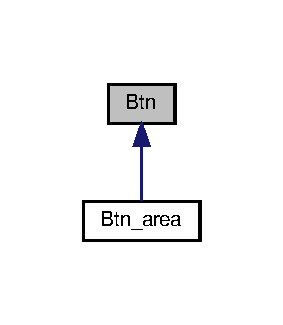
\includegraphics[width=136pt]{classRET__config_1_1Btn__inherit__graph}
\end{center}
\end{figure}
\subsection*{Public Member Functions}
\begin{DoxyCompactItemize}
\item 
def \hyperlink{classRET__config_1_1Btn_ab98adcd48a87d3624f5913a189a7b329}{\+\_\+\+\_\+init\+\_\+\+\_\+} (self, \hyperlink{classRET__config_1_1Btn_ab74e6bf80237ddc4109968cedc58c151}{name}, \hyperlink{classRET__config_1_1Btn_a9336ebf25087d91c818ee6e9ec29f8c1}{x}, \hyperlink{classRET__config_1_1Btn_a2fb1c5cf58867b5bbc9a1b145a86f3a0}{y}, \hyperlink{classRET__config_1_1Btn_a25ed1bcb423b0b7200f485fc5ff71c8e}{z})
\begin{DoxyCompactList}\small\item\em The \hyperlink{classRET__config_1_1Btn}{Btn} base class initializer. \end{DoxyCompactList}\end{DoxyCompactItemize}
\subsection*{Public Attributes}
\begin{DoxyCompactItemize}
\item 
\hyperlink{classRET__config_1_1Btn_ab74e6bf80237ddc4109968cedc58c151}{name}
\item 
\hyperlink{classRET__config_1_1Btn_a9336ebf25087d91c818ee6e9ec29f8c1}{x}
\item 
\hyperlink{classRET__config_1_1Btn_a2fb1c5cf58867b5bbc9a1b145a86f3a0}{y}
\item 
\hyperlink{classRET__config_1_1Btn_a25ed1bcb423b0b7200f485fc5ff71c8e}{z}
\end{DoxyCompactItemize}


\subsection{Detailed Description}
The \hyperlink{classRET__config_1_1Btn}{Btn} base class. 

Defines the base class utilized by all buttons. 

\subsection{Constructor \& Destructor Documentation}
\mbox{\Hypertarget{classRET__config_1_1Btn_ab98adcd48a87d3624f5913a189a7b329}\label{classRET__config_1_1Btn_ab98adcd48a87d3624f5913a189a7b329}} 
\index{R\+E\+T\+\_\+config\+::\+Btn@{R\+E\+T\+\_\+config\+::\+Btn}!\+\_\+\+\_\+init\+\_\+\+\_\+@{\+\_\+\+\_\+init\+\_\+\+\_\+}}
\index{\+\_\+\+\_\+init\+\_\+\+\_\+@{\+\_\+\+\_\+init\+\_\+\+\_\+}!R\+E\+T\+\_\+config\+::\+Btn@{R\+E\+T\+\_\+config\+::\+Btn}}
\subsubsection{\texorpdfstring{\+\_\+\+\_\+init\+\_\+\+\_\+()}{\_\_init\_\_()}}
{\footnotesize\ttfamily def \+\_\+\+\_\+init\+\_\+\+\_\+ (\begin{DoxyParamCaption}\item[{}]{self,  }\item[{}]{name,  }\item[{}]{x,  }\item[{}]{y,  }\item[{}]{z }\end{DoxyParamCaption})}



The \hyperlink{classRET__config_1_1Btn}{Btn} base class initializer. 


\begin{DoxyParams}{Parameters}
{\em name} & The name of the \hyperlink{classRET__config_1_1Btn}{Btn}. \\
\hline
{\em x} & The x coordinate of the button. \\
\hline
{\em y} & The y coordinate of the button. \\
\hline
{\em z} & The z coordinate of the button. \\
\hline
\end{DoxyParams}
\begin{DoxyReturn}{Returns}
An instance of the \hyperlink{classRET__config_1_1Btn}{Btn} class initialized with the specified name. 
\end{DoxyReturn}


\subsection{Member Data Documentation}
\mbox{\Hypertarget{classRET__config_1_1Btn_ab74e6bf80237ddc4109968cedc58c151}\label{classRET__config_1_1Btn_ab74e6bf80237ddc4109968cedc58c151}} 
\index{R\+E\+T\+\_\+config\+::\+Btn@{R\+E\+T\+\_\+config\+::\+Btn}!name@{name}}
\index{name@{name}!R\+E\+T\+\_\+config\+::\+Btn@{R\+E\+T\+\_\+config\+::\+Btn}}
\subsubsection{\texorpdfstring{name}{name}}
{\footnotesize\ttfamily name}

\mbox{\Hypertarget{classRET__config_1_1Btn_a9336ebf25087d91c818ee6e9ec29f8c1}\label{classRET__config_1_1Btn_a9336ebf25087d91c818ee6e9ec29f8c1}} 
\index{R\+E\+T\+\_\+config\+::\+Btn@{R\+E\+T\+\_\+config\+::\+Btn}!x@{x}}
\index{x@{x}!R\+E\+T\+\_\+config\+::\+Btn@{R\+E\+T\+\_\+config\+::\+Btn}}
\subsubsection{\texorpdfstring{x}{x}}
{\footnotesize\ttfamily x}

\mbox{\Hypertarget{classRET__config_1_1Btn_a2fb1c5cf58867b5bbc9a1b145a86f3a0}\label{classRET__config_1_1Btn_a2fb1c5cf58867b5bbc9a1b145a86f3a0}} 
\index{R\+E\+T\+\_\+config\+::\+Btn@{R\+E\+T\+\_\+config\+::\+Btn}!y@{y}}
\index{y@{y}!R\+E\+T\+\_\+config\+::\+Btn@{R\+E\+T\+\_\+config\+::\+Btn}}
\subsubsection{\texorpdfstring{y}{y}}
{\footnotesize\ttfamily y}

\mbox{\Hypertarget{classRET__config_1_1Btn_a25ed1bcb423b0b7200f485fc5ff71c8e}\label{classRET__config_1_1Btn_a25ed1bcb423b0b7200f485fc5ff71c8e}} 
\index{R\+E\+T\+\_\+config\+::\+Btn@{R\+E\+T\+\_\+config\+::\+Btn}!z@{z}}
\index{z@{z}!R\+E\+T\+\_\+config\+::\+Btn@{R\+E\+T\+\_\+config\+::\+Btn}}
\subsubsection{\texorpdfstring{z}{z}}
{\footnotesize\ttfamily z}



The documentation for this class was generated from the following file\+:\begin{DoxyCompactItemize}
\item 
/home/ret/workspaces/ret/src/ret/scripts/\hyperlink{RET__config_8py}{R\+E\+T\+\_\+config.\+py}\end{DoxyCompactItemize}

\hypertarget{classRET__config_1_1Btn__area}{}\section{Btn\+\_\+area Class Reference}
\label{classRET__config_1_1Btn__area}\index{Btn\+\_\+area@{Btn\+\_\+area}}


The \hyperlink{classRET__config_1_1Btn__area}{Btn\+\_\+area} class.  




Inheritance diagram for Btn\+\_\+area\+:
\nopagebreak
\begin{figure}[H]
\begin{center}
\leavevmode
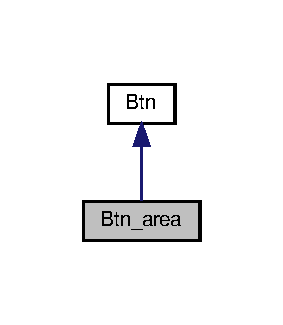
\includegraphics[width=136pt]{classRET__config_1_1Btn__area__inherit__graph}
\end{center}
\end{figure}


Collaboration diagram for Btn\+\_\+area\+:
\nopagebreak
\begin{figure}[H]
\begin{center}
\leavevmode
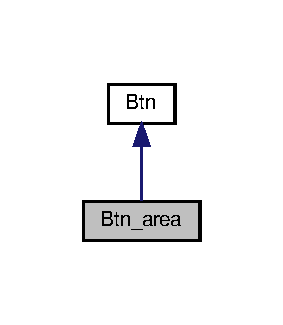
\includegraphics[width=136pt]{classRET__config_1_1Btn__area__coll__graph}
\end{center}
\end{figure}
\subsection*{Public Member Functions}
\begin{DoxyCompactItemize}
\item 
def \hyperlink{classRET__config_1_1Btn__area_a950cef8a3171324f99f08291a29675d0}{\+\_\+\+\_\+init\+\_\+\+\_\+} (self, \hyperlink{classRET__config_1_1Btn}{Btn}, \hyperlink{classRET__config_1_1Btn__area_aacddc911cdfe5cd5ec97b084754542d4}{dx}, \hyperlink{classRET__config_1_1Btn__area_a22b1a06ae09d552a5ca668a07885ebf1}{dy}, \hyperlink{classRET__config_1_1Btn__area_a71f0caccd6959b358543ee9cdc9b9c3e}{dz})
\begin{DoxyCompactList}\small\item\em The \hyperlink{classRET__config_1_1Btn__area}{Btn\+\_\+area} base class initializer. \end{DoxyCompactList}\end{DoxyCompactItemize}
\subsection*{Public Attributes}
\begin{DoxyCompactItemize}
\item 
\hyperlink{classRET__config_1_1Btn__area_aacddc911cdfe5cd5ec97b084754542d4}{dx}
\item 
\hyperlink{classRET__config_1_1Btn__area_a22b1a06ae09d552a5ca668a07885ebf1}{dy}
\item 
\hyperlink{classRET__config_1_1Btn__area_a71f0caccd6959b358543ee9cdc9b9c3e}{dz}
\item 
\hyperlink{classRET__config_1_1Btn__area_aef852a503e1c3a4a136a08fb7ccfdf34}{end\+\_\+effector\+\_\+inside\+\_\+area}
\item 
\hyperlink{classRET__config_1_1Btn__area_a253bff6f53fd0cf42fe16fae256db20d}{lower\+\_\+x}
\item 
\hyperlink{classRET__config_1_1Btn__area_abde8ef835f0f5ec35e19a41ea81635b9}{lower\+\_\+y}
\item 
\hyperlink{classRET__config_1_1Btn__area_aafde5bf16bebefaac407edbf1a82be2c}{lower\+\_\+z}
\item 
\hyperlink{classRET__config_1_1Btn__area_ab74e6bf80237ddc4109968cedc58c151}{name}
\item 
\hyperlink{classRET__config_1_1Btn__area_a83a922996b3291335a4a7e12ec0352c5}{send\+\_\+message\+\_\+entering\+\_\+area}
\item 
\hyperlink{classRET__config_1_1Btn__area_a1093600f9685edcc41b8846f856d4575}{send\+\_\+message\+\_\+leaving\+\_\+area}
\item 
\hyperlink{classRET__config_1_1Btn__area_a9187fb0045f227875406717af543604d}{time\+\_\+end\+\_\+effector\+\_\+entering\+\_\+area}
\item 
\hyperlink{classRET__config_1_1Btn__area_ac9034ace22eed6b580e2c01ba5b2e71d}{time\+\_\+end\+\_\+effector\+\_\+leaving\+\_\+area}
\item 
\hyperlink{classRET__config_1_1Btn__area_a5fc95389df55bf4e81e2c0eec403a7ee}{upper\+\_\+x}
\item 
\hyperlink{classRET__config_1_1Btn__area_af3d0698df9e9a8a5fb89a126a503bfbd}{upper\+\_\+y}
\item 
\hyperlink{classRET__config_1_1Btn__area_a5180143a531a7caaefecdd56d378de44}{upper\+\_\+z}
\item 
\hyperlink{classRET__config_1_1Btn__area_a9336ebf25087d91c818ee6e9ec29f8c1}{x}
\item 
\hyperlink{classRET__config_1_1Btn__area_a2fb1c5cf58867b5bbc9a1b145a86f3a0}{y}
\item 
\hyperlink{classRET__config_1_1Btn__area_a25ed1bcb423b0b7200f485fc5ff71c8e}{z}
\end{DoxyCompactItemize}


\subsection{Detailed Description}
The \hyperlink{classRET__config_1_1Btn__area}{Btn\+\_\+area} class. 

Provide access to the button\+\_\+area\textquotesingle{}s. 

\subsection{Constructor \& Destructor Documentation}
\mbox{\Hypertarget{classRET__config_1_1Btn__area_a950cef8a3171324f99f08291a29675d0}\label{classRET__config_1_1Btn__area_a950cef8a3171324f99f08291a29675d0}} 
\index{R\+E\+T\+\_\+config\+::\+Btn\+\_\+area@{R\+E\+T\+\_\+config\+::\+Btn\+\_\+area}!\+\_\+\+\_\+init\+\_\+\+\_\+@{\+\_\+\+\_\+init\+\_\+\+\_\+}}
\index{\+\_\+\+\_\+init\+\_\+\+\_\+@{\+\_\+\+\_\+init\+\_\+\+\_\+}!R\+E\+T\+\_\+config\+::\+Btn\+\_\+area@{R\+E\+T\+\_\+config\+::\+Btn\+\_\+area}}
\subsubsection{\texorpdfstring{\+\_\+\+\_\+init\+\_\+\+\_\+()}{\_\_init\_\_()}}
{\footnotesize\ttfamily def \+\_\+\+\_\+init\+\_\+\+\_\+ (\begin{DoxyParamCaption}\item[{}]{self,  }\item[{}]{Btn,  }\item[{}]{dx,  }\item[{}]{dy,  }\item[{}]{dz }\end{DoxyParamCaption})}



The \hyperlink{classRET__config_1_1Btn__area}{Btn\+\_\+area} base class initializer. 


\begin{DoxyParams}{Parameters}
{\em \hyperlink{classRET__config_1_1Btn}{Btn}} & The \hyperlink{classRET__config_1_1Btn}{Btn} we are defining the area of. \\
\hline
{\em dx} & The delta on x we are defining for the button area. \\
\hline
{\em dy} & The delta on y we are defining for the button area. \\
\hline
{\em dz} & The delta on z we are defining for the button area. \\
\hline
\end{DoxyParams}
\begin{DoxyReturn}{Returns}
An instance of the \hyperlink{classRET__config_1_1Btn__area}{Btn\+\_\+area} class initialized with the specified name. 
\end{DoxyReturn}


\subsection{Member Data Documentation}
\mbox{\Hypertarget{classRET__config_1_1Btn__area_aacddc911cdfe5cd5ec97b084754542d4}\label{classRET__config_1_1Btn__area_aacddc911cdfe5cd5ec97b084754542d4}} 
\index{R\+E\+T\+\_\+config\+::\+Btn\+\_\+area@{R\+E\+T\+\_\+config\+::\+Btn\+\_\+area}!dx@{dx}}
\index{dx@{dx}!R\+E\+T\+\_\+config\+::\+Btn\+\_\+area@{R\+E\+T\+\_\+config\+::\+Btn\+\_\+area}}
\subsubsection{\texorpdfstring{dx}{dx}}
{\footnotesize\ttfamily dx}

\mbox{\Hypertarget{classRET__config_1_1Btn__area_a22b1a06ae09d552a5ca668a07885ebf1}\label{classRET__config_1_1Btn__area_a22b1a06ae09d552a5ca668a07885ebf1}} 
\index{R\+E\+T\+\_\+config\+::\+Btn\+\_\+area@{R\+E\+T\+\_\+config\+::\+Btn\+\_\+area}!dy@{dy}}
\index{dy@{dy}!R\+E\+T\+\_\+config\+::\+Btn\+\_\+area@{R\+E\+T\+\_\+config\+::\+Btn\+\_\+area}}
\subsubsection{\texorpdfstring{dy}{dy}}
{\footnotesize\ttfamily dy}

\mbox{\Hypertarget{classRET__config_1_1Btn__area_a71f0caccd6959b358543ee9cdc9b9c3e}\label{classRET__config_1_1Btn__area_a71f0caccd6959b358543ee9cdc9b9c3e}} 
\index{R\+E\+T\+\_\+config\+::\+Btn\+\_\+area@{R\+E\+T\+\_\+config\+::\+Btn\+\_\+area}!dz@{dz}}
\index{dz@{dz}!R\+E\+T\+\_\+config\+::\+Btn\+\_\+area@{R\+E\+T\+\_\+config\+::\+Btn\+\_\+area}}
\subsubsection{\texorpdfstring{dz}{dz}}
{\footnotesize\ttfamily dz}

\mbox{\Hypertarget{classRET__config_1_1Btn__area_aef852a503e1c3a4a136a08fb7ccfdf34}\label{classRET__config_1_1Btn__area_aef852a503e1c3a4a136a08fb7ccfdf34}} 
\index{R\+E\+T\+\_\+config\+::\+Btn\+\_\+area@{R\+E\+T\+\_\+config\+::\+Btn\+\_\+area}!end\+\_\+effector\+\_\+inside\+\_\+area@{end\+\_\+effector\+\_\+inside\+\_\+area}}
\index{end\+\_\+effector\+\_\+inside\+\_\+area@{end\+\_\+effector\+\_\+inside\+\_\+area}!R\+E\+T\+\_\+config\+::\+Btn\+\_\+area@{R\+E\+T\+\_\+config\+::\+Btn\+\_\+area}}
\subsubsection{\texorpdfstring{end\+\_\+effector\+\_\+inside\+\_\+area}{end\_effector\_inside\_area}}
{\footnotesize\ttfamily end\+\_\+effector\+\_\+inside\+\_\+area}

\mbox{\Hypertarget{classRET__config_1_1Btn__area_a253bff6f53fd0cf42fe16fae256db20d}\label{classRET__config_1_1Btn__area_a253bff6f53fd0cf42fe16fae256db20d}} 
\index{R\+E\+T\+\_\+config\+::\+Btn\+\_\+area@{R\+E\+T\+\_\+config\+::\+Btn\+\_\+area}!lower\+\_\+x@{lower\+\_\+x}}
\index{lower\+\_\+x@{lower\+\_\+x}!R\+E\+T\+\_\+config\+::\+Btn\+\_\+area@{R\+E\+T\+\_\+config\+::\+Btn\+\_\+area}}
\subsubsection{\texorpdfstring{lower\+\_\+x}{lower\_x}}
{\footnotesize\ttfamily lower\+\_\+x}

\mbox{\Hypertarget{classRET__config_1_1Btn__area_abde8ef835f0f5ec35e19a41ea81635b9}\label{classRET__config_1_1Btn__area_abde8ef835f0f5ec35e19a41ea81635b9}} 
\index{R\+E\+T\+\_\+config\+::\+Btn\+\_\+area@{R\+E\+T\+\_\+config\+::\+Btn\+\_\+area}!lower\+\_\+y@{lower\+\_\+y}}
\index{lower\+\_\+y@{lower\+\_\+y}!R\+E\+T\+\_\+config\+::\+Btn\+\_\+area@{R\+E\+T\+\_\+config\+::\+Btn\+\_\+area}}
\subsubsection{\texorpdfstring{lower\+\_\+y}{lower\_y}}
{\footnotesize\ttfamily lower\+\_\+y}

\mbox{\Hypertarget{classRET__config_1_1Btn__area_aafde5bf16bebefaac407edbf1a82be2c}\label{classRET__config_1_1Btn__area_aafde5bf16bebefaac407edbf1a82be2c}} 
\index{R\+E\+T\+\_\+config\+::\+Btn\+\_\+area@{R\+E\+T\+\_\+config\+::\+Btn\+\_\+area}!lower\+\_\+z@{lower\+\_\+z}}
\index{lower\+\_\+z@{lower\+\_\+z}!R\+E\+T\+\_\+config\+::\+Btn\+\_\+area@{R\+E\+T\+\_\+config\+::\+Btn\+\_\+area}}
\subsubsection{\texorpdfstring{lower\+\_\+z}{lower\_z}}
{\footnotesize\ttfamily lower\+\_\+z}

\mbox{\Hypertarget{classRET__config_1_1Btn__area_ab74e6bf80237ddc4109968cedc58c151}\label{classRET__config_1_1Btn__area_ab74e6bf80237ddc4109968cedc58c151}} 
\index{R\+E\+T\+\_\+config\+::\+Btn\+\_\+area@{R\+E\+T\+\_\+config\+::\+Btn\+\_\+area}!name@{name}}
\index{name@{name}!R\+E\+T\+\_\+config\+::\+Btn\+\_\+area@{R\+E\+T\+\_\+config\+::\+Btn\+\_\+area}}
\subsubsection{\texorpdfstring{name}{name}}
{\footnotesize\ttfamily name}

\mbox{\Hypertarget{classRET__config_1_1Btn__area_a83a922996b3291335a4a7e12ec0352c5}\label{classRET__config_1_1Btn__area_a83a922996b3291335a4a7e12ec0352c5}} 
\index{R\+E\+T\+\_\+config\+::\+Btn\+\_\+area@{R\+E\+T\+\_\+config\+::\+Btn\+\_\+area}!send\+\_\+message\+\_\+entering\+\_\+area@{send\+\_\+message\+\_\+entering\+\_\+area}}
\index{send\+\_\+message\+\_\+entering\+\_\+area@{send\+\_\+message\+\_\+entering\+\_\+area}!R\+E\+T\+\_\+config\+::\+Btn\+\_\+area@{R\+E\+T\+\_\+config\+::\+Btn\+\_\+area}}
\subsubsection{\texorpdfstring{send\+\_\+message\+\_\+entering\+\_\+area}{send\_message\_entering\_area}}
{\footnotesize\ttfamily send\+\_\+message\+\_\+entering\+\_\+area}

\mbox{\Hypertarget{classRET__config_1_1Btn__area_a1093600f9685edcc41b8846f856d4575}\label{classRET__config_1_1Btn__area_a1093600f9685edcc41b8846f856d4575}} 
\index{R\+E\+T\+\_\+config\+::\+Btn\+\_\+area@{R\+E\+T\+\_\+config\+::\+Btn\+\_\+area}!send\+\_\+message\+\_\+leaving\+\_\+area@{send\+\_\+message\+\_\+leaving\+\_\+area}}
\index{send\+\_\+message\+\_\+leaving\+\_\+area@{send\+\_\+message\+\_\+leaving\+\_\+area}!R\+E\+T\+\_\+config\+::\+Btn\+\_\+area@{R\+E\+T\+\_\+config\+::\+Btn\+\_\+area}}
\subsubsection{\texorpdfstring{send\+\_\+message\+\_\+leaving\+\_\+area}{send\_message\_leaving\_area}}
{\footnotesize\ttfamily send\+\_\+message\+\_\+leaving\+\_\+area}

\mbox{\Hypertarget{classRET__config_1_1Btn__area_a9187fb0045f227875406717af543604d}\label{classRET__config_1_1Btn__area_a9187fb0045f227875406717af543604d}} 
\index{R\+E\+T\+\_\+config\+::\+Btn\+\_\+area@{R\+E\+T\+\_\+config\+::\+Btn\+\_\+area}!time\+\_\+end\+\_\+effector\+\_\+entering\+\_\+area@{time\+\_\+end\+\_\+effector\+\_\+entering\+\_\+area}}
\index{time\+\_\+end\+\_\+effector\+\_\+entering\+\_\+area@{time\+\_\+end\+\_\+effector\+\_\+entering\+\_\+area}!R\+E\+T\+\_\+config\+::\+Btn\+\_\+area@{R\+E\+T\+\_\+config\+::\+Btn\+\_\+area}}
\subsubsection{\texorpdfstring{time\+\_\+end\+\_\+effector\+\_\+entering\+\_\+area}{time\_end\_effector\_entering\_area}}
{\footnotesize\ttfamily time\+\_\+end\+\_\+effector\+\_\+entering\+\_\+area}

\mbox{\Hypertarget{classRET__config_1_1Btn__area_ac9034ace22eed6b580e2c01ba5b2e71d}\label{classRET__config_1_1Btn__area_ac9034ace22eed6b580e2c01ba5b2e71d}} 
\index{R\+E\+T\+\_\+config\+::\+Btn\+\_\+area@{R\+E\+T\+\_\+config\+::\+Btn\+\_\+area}!time\+\_\+end\+\_\+effector\+\_\+leaving\+\_\+area@{time\+\_\+end\+\_\+effector\+\_\+leaving\+\_\+area}}
\index{time\+\_\+end\+\_\+effector\+\_\+leaving\+\_\+area@{time\+\_\+end\+\_\+effector\+\_\+leaving\+\_\+area}!R\+E\+T\+\_\+config\+::\+Btn\+\_\+area@{R\+E\+T\+\_\+config\+::\+Btn\+\_\+area}}
\subsubsection{\texorpdfstring{time\+\_\+end\+\_\+effector\+\_\+leaving\+\_\+area}{time\_end\_effector\_leaving\_area}}
{\footnotesize\ttfamily time\+\_\+end\+\_\+effector\+\_\+leaving\+\_\+area}

\mbox{\Hypertarget{classRET__config_1_1Btn__area_a5fc95389df55bf4e81e2c0eec403a7ee}\label{classRET__config_1_1Btn__area_a5fc95389df55bf4e81e2c0eec403a7ee}} 
\index{R\+E\+T\+\_\+config\+::\+Btn\+\_\+area@{R\+E\+T\+\_\+config\+::\+Btn\+\_\+area}!upper\+\_\+x@{upper\+\_\+x}}
\index{upper\+\_\+x@{upper\+\_\+x}!R\+E\+T\+\_\+config\+::\+Btn\+\_\+area@{R\+E\+T\+\_\+config\+::\+Btn\+\_\+area}}
\subsubsection{\texorpdfstring{upper\+\_\+x}{upper\_x}}
{\footnotesize\ttfamily upper\+\_\+x}

\mbox{\Hypertarget{classRET__config_1_1Btn__area_af3d0698df9e9a8a5fb89a126a503bfbd}\label{classRET__config_1_1Btn__area_af3d0698df9e9a8a5fb89a126a503bfbd}} 
\index{R\+E\+T\+\_\+config\+::\+Btn\+\_\+area@{R\+E\+T\+\_\+config\+::\+Btn\+\_\+area}!upper\+\_\+y@{upper\+\_\+y}}
\index{upper\+\_\+y@{upper\+\_\+y}!R\+E\+T\+\_\+config\+::\+Btn\+\_\+area@{R\+E\+T\+\_\+config\+::\+Btn\+\_\+area}}
\subsubsection{\texorpdfstring{upper\+\_\+y}{upper\_y}}
{\footnotesize\ttfamily upper\+\_\+y}

\mbox{\Hypertarget{classRET__config_1_1Btn__area_a5180143a531a7caaefecdd56d378de44}\label{classRET__config_1_1Btn__area_a5180143a531a7caaefecdd56d378de44}} 
\index{R\+E\+T\+\_\+config\+::\+Btn\+\_\+area@{R\+E\+T\+\_\+config\+::\+Btn\+\_\+area}!upper\+\_\+z@{upper\+\_\+z}}
\index{upper\+\_\+z@{upper\+\_\+z}!R\+E\+T\+\_\+config\+::\+Btn\+\_\+area@{R\+E\+T\+\_\+config\+::\+Btn\+\_\+area}}
\subsubsection{\texorpdfstring{upper\+\_\+z}{upper\_z}}
{\footnotesize\ttfamily upper\+\_\+z}

\mbox{\Hypertarget{classRET__config_1_1Btn__area_a9336ebf25087d91c818ee6e9ec29f8c1}\label{classRET__config_1_1Btn__area_a9336ebf25087d91c818ee6e9ec29f8c1}} 
\index{R\+E\+T\+\_\+config\+::\+Btn\+\_\+area@{R\+E\+T\+\_\+config\+::\+Btn\+\_\+area}!x@{x}}
\index{x@{x}!R\+E\+T\+\_\+config\+::\+Btn\+\_\+area@{R\+E\+T\+\_\+config\+::\+Btn\+\_\+area}}
\subsubsection{\texorpdfstring{x}{x}}
{\footnotesize\ttfamily x}

\mbox{\Hypertarget{classRET__config_1_1Btn__area_a2fb1c5cf58867b5bbc9a1b145a86f3a0}\label{classRET__config_1_1Btn__area_a2fb1c5cf58867b5bbc9a1b145a86f3a0}} 
\index{R\+E\+T\+\_\+config\+::\+Btn\+\_\+area@{R\+E\+T\+\_\+config\+::\+Btn\+\_\+area}!y@{y}}
\index{y@{y}!R\+E\+T\+\_\+config\+::\+Btn\+\_\+area@{R\+E\+T\+\_\+config\+::\+Btn\+\_\+area}}
\subsubsection{\texorpdfstring{y}{y}}
{\footnotesize\ttfamily y}

\mbox{\Hypertarget{classRET__config_1_1Btn__area_a25ed1bcb423b0b7200f485fc5ff71c8e}\label{classRET__config_1_1Btn__area_a25ed1bcb423b0b7200f485fc5ff71c8e}} 
\index{R\+E\+T\+\_\+config\+::\+Btn\+\_\+area@{R\+E\+T\+\_\+config\+::\+Btn\+\_\+area}!z@{z}}
\index{z@{z}!R\+E\+T\+\_\+config\+::\+Btn\+\_\+area@{R\+E\+T\+\_\+config\+::\+Btn\+\_\+area}}
\subsubsection{\texorpdfstring{z}{z}}
{\footnotesize\ttfamily z}



The documentation for this class was generated from the following file\+:\begin{DoxyCompactItemize}
\item 
/home/ret/workspaces/ret/src/ret/scripts/\hyperlink{RET__config_8py}{R\+E\+T\+\_\+config.\+py}\end{DoxyCompactItemize}

\hypertarget{classButton__Masher__Application__Output_1_1Button__Masher__Application__node__listener}{}\section{Button\+\_\+\+Masher\+\_\+\+Application\+\_\+node\+\_\+listener Class Reference}
\label{classButton__Masher__Application__Output_1_1Button__Masher__Application__node__listener}\index{Button\+\_\+\+Masher\+\_\+\+Application\+\_\+node\+\_\+listener@{Button\+\_\+\+Masher\+\_\+\+Application\+\_\+node\+\_\+listener}}


The \hyperlink{classButton__Masher__Application__Output_1_1Button__Masher__Application__node__listener}{Button\+\_\+\+Masher\+\_\+\+Application\+\_\+node\+\_\+listener} base class.  




Inheritance diagram for Button\+\_\+\+Masher\+\_\+\+Application\+\_\+node\+\_\+listener\+:
\nopagebreak
\begin{figure}[H]
\begin{center}
\leavevmode
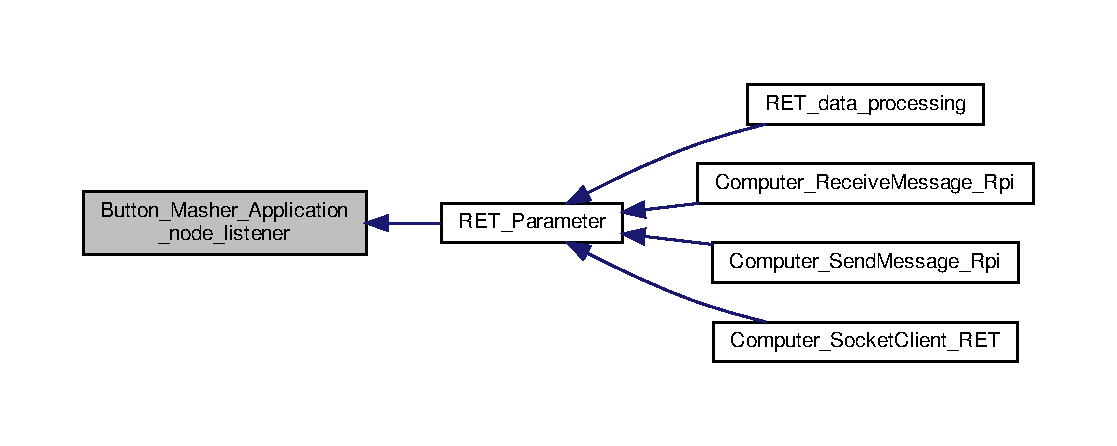
\includegraphics[width=350pt]{classButton__Masher__Application__Output_1_1Button__Masher__Application__node__listener__inherit__graph}
\end{center}
\end{figure}
\subsection*{Public Member Functions}
\begin{DoxyCompactItemize}
\item 
def \hyperlink{classButton__Masher__Application__Output_1_1Button__Masher__Application__node__listener_ae64f0875afe3067b97ba370b354b9213}{\+\_\+\+\_\+init\+\_\+\+\_\+} (self)
\begin{DoxyCompactList}\small\item\em The \hyperlink{classButton__Masher__Application__Output_1_1Button__Masher__Application__node__listener}{Button\+\_\+\+Masher\+\_\+\+Application\+\_\+node\+\_\+listener} base class initializer. \end{DoxyCompactList}\item 
def \hyperlink{classButton__Masher__Application__Output_1_1Button__Masher__Application__node__listener_ab35c2e69050a4f7d87cf90a41f087211}{additional\+\_\+callback} (self, diagnostics)
\item 
def \hyperlink{classButton__Masher__Application__Output_1_1Button__Masher__Application__node__listener_ab3b9e5b2975cf90154645eee1c579708}{diagnostics\+\_\+callback} (self, diagnostics)
\begin{DoxyCompactList}\small\item\em Retrieves the \hyperlink{namespaceButton__Masher__Application__Output}{Button\+\_\+\+Masher\+\_\+\+Application\+\_\+\+Output}. \end{DoxyCompactList}\item 
def \hyperlink{classButton__Masher__Application__Output_1_1Button__Masher__Application__node__listener_a04fc3ce521383ebf5abcc970f6d403b3}{print\+\_\+all\+\_\+info} (self)
\item 
def \hyperlink{classButton__Masher__Application__Output_1_1Button__Masher__Application__node__listener_a123cdc0332063476801ee93d615ea911}{print\+\_\+end\+\_\+effector\+\_\+position\+\_\+information} (self)
\begin{DoxyCompactList}\small\item\em Retrieves the \hyperlink{namespaceButton__Masher__Application__Output}{Button\+\_\+\+Masher\+\_\+\+Application\+\_\+\+Output}. \end{DoxyCompactList}\item 
def \hyperlink{classButton__Masher__Application__Output_1_1Button__Masher__Application__node__listener_a0897f4dea41dd51e61ea2d7a6eaf44c7}{write\+\_\+info\+\_\+json\+\_\+into\+\_\+db} (self, \hyperlink{classButton__Masher__Application__Output_1_1Button__Masher__Application__node__listener_ad5bc32b75da65fe60067f501a4bb6665}{client})
\item 
def \hyperlink{classButton__Masher__Application__Output_1_1Button__Masher__Application__node__listener_af1481d5ed69bf66fb8f4356694ae23b9}{write\+\_\+info\+\_\+json\+\_\+into\+\_\+db\+\_\+additional} (self, \hyperlink{classButton__Masher__Application__Output_1_1Button__Masher__Application__node__listener_ad5bc32b75da65fe60067f501a4bb6665}{client})
\item 
def \hyperlink{classButton__Masher__Application__Output_1_1Button__Masher__Application__node__listener_aa073b1c8f4b4c6517f35ade17ed85dd6}{write\+\_\+into\+\_\+db} (self, \hyperlink{classButton__Masher__Application__Output_1_1Button__Masher__Application__node__listener_ad5bc32b75da65fe60067f501a4bb6665}{client})
\end{DoxyCompactItemize}
\subsection*{Public Attributes}
\begin{DoxyCompactItemize}
\item 
\hyperlink{classButton__Masher__Application__Output_1_1Button__Masher__Application__node__listener_a4141d2c72ff71283722dda8c431a48d6}{actual\+\_\+state}
\item 
\hyperlink{classButton__Masher__Application__Output_1_1Button__Masher__Application__node__listener_ad3dcada5e11b20f5dc822acf601a645b}{cartesian\+\_\+position\+\_\+end\+\_\+effector}
\item 
\hyperlink{classButton__Masher__Application__Output_1_1Button__Masher__Application__node__listener_ad5bc32b75da65fe60067f501a4bb6665}{client}
\item 
\hyperlink{classButton__Masher__Application__Output_1_1Button__Masher__Application__node__listener_a511ae0b1c13f95e5f08f1a0dd3da3d93}{data}
\item 
\hyperlink{classButton__Masher__Application__Output_1_1Button__Masher__Application__node__listener_a547b75f681b266f91f9cc485c2f3b714}{diagnostics\+\_\+sub}
\begin{DoxyCompactList}\small\item\em add the listening of the joint position node see if it works \end{DoxyCompactList}\item 
\hyperlink{classButton__Masher__Application__Output_1_1Button__Masher__Application__node__listener_a4e790a9b608d07d8c1273ce749657a55}{encoded\+\_\+state}
\item 
\hyperlink{classButton__Masher__Application__Output_1_1Button__Masher__Application__node__listener_a954c5caf30928503ff36b24cc6d6414d}{error\+\_\+state}
\item 
\hyperlink{classButton__Masher__Application__Output_1_1Button__Masher__Application__node__listener_ab67dc6cccbf6aeaeeeef8690bacd403c}{temperature}
\item 
\hyperlink{classButton__Masher__Application__Output_1_1Button__Masher__Application__node__listener_aca0b5e2418a650b09d5b7b497bbeecfc}{time\+\_\+info}
\item 
\hyperlink{classButton__Masher__Application__Output_1_1Button__Masher__Application__node__listener_aa1a8261d8fb901476651f1666f993d4b}{voltage}
\item 
\hyperlink{classButton__Masher__Application__Output_1_1Button__Masher__Application__node__listener_a9336ebf25087d91c818ee6e9ec29f8c1}{x}
\item 
\hyperlink{classButton__Masher__Application__Output_1_1Button__Masher__Application__node__listener_a2fb1c5cf58867b5bbc9a1b145a86f3a0}{y}
\item 
\hyperlink{classButton__Masher__Application__Output_1_1Button__Masher__Application__node__listener_a25ed1bcb423b0b7200f485fc5ff71c8e}{z}
\end{DoxyCompactItemize}


\subsection{Detailed Description}
The \hyperlink{classButton__Masher__Application__Output_1_1Button__Masher__Application__node__listener}{Button\+\_\+\+Masher\+\_\+\+Application\+\_\+node\+\_\+listener} base class. 

Defines the base class used by the R\+ET to subscribe to the /tool\+\_\+pose topic and get the end effector cartesian position. 

\subsection{Constructor \& Destructor Documentation}
\mbox{\Hypertarget{classButton__Masher__Application__Output_1_1Button__Masher__Application__node__listener_ae64f0875afe3067b97ba370b354b9213}\label{classButton__Masher__Application__Output_1_1Button__Masher__Application__node__listener_ae64f0875afe3067b97ba370b354b9213}} 
\index{Button\+\_\+\+Masher\+\_\+\+Application\+\_\+\+Output\+::\+Button\+\_\+\+Masher\+\_\+\+Application\+\_\+node\+\_\+listener@{Button\+\_\+\+Masher\+\_\+\+Application\+\_\+\+Output\+::\+Button\+\_\+\+Masher\+\_\+\+Application\+\_\+node\+\_\+listener}!\+\_\+\+\_\+init\+\_\+\+\_\+@{\+\_\+\+\_\+init\+\_\+\+\_\+}}
\index{\+\_\+\+\_\+init\+\_\+\+\_\+@{\+\_\+\+\_\+init\+\_\+\+\_\+}!Button\+\_\+\+Masher\+\_\+\+Application\+\_\+\+Output\+::\+Button\+\_\+\+Masher\+\_\+\+Application\+\_\+node\+\_\+listener@{Button\+\_\+\+Masher\+\_\+\+Application\+\_\+\+Output\+::\+Button\+\_\+\+Masher\+\_\+\+Application\+\_\+node\+\_\+listener}}
\subsubsection{\texorpdfstring{\+\_\+\+\_\+init\+\_\+\+\_\+()}{\_\_init\_\_()}}
{\footnotesize\ttfamily def \+\_\+\+\_\+init\+\_\+\+\_\+ (\begin{DoxyParamCaption}\item[{}]{self }\end{DoxyParamCaption})}



The \hyperlink{classButton__Masher__Application__Output_1_1Button__Masher__Application__node__listener}{Button\+\_\+\+Masher\+\_\+\+Application\+\_\+node\+\_\+listener} base class initializer. 



\subsection{Member Function Documentation}
\mbox{\Hypertarget{classButton__Masher__Application__Output_1_1Button__Masher__Application__node__listener_ab35c2e69050a4f7d87cf90a41f087211}\label{classButton__Masher__Application__Output_1_1Button__Masher__Application__node__listener_ab35c2e69050a4f7d87cf90a41f087211}} 
\index{Button\+\_\+\+Masher\+\_\+\+Application\+\_\+\+Output\+::\+Button\+\_\+\+Masher\+\_\+\+Application\+\_\+node\+\_\+listener@{Button\+\_\+\+Masher\+\_\+\+Application\+\_\+\+Output\+::\+Button\+\_\+\+Masher\+\_\+\+Application\+\_\+node\+\_\+listener}!additional\+\_\+callback@{additional\+\_\+callback}}
\index{additional\+\_\+callback@{additional\+\_\+callback}!Button\+\_\+\+Masher\+\_\+\+Application\+\_\+\+Output\+::\+Button\+\_\+\+Masher\+\_\+\+Application\+\_\+node\+\_\+listener@{Button\+\_\+\+Masher\+\_\+\+Application\+\_\+\+Output\+::\+Button\+\_\+\+Masher\+\_\+\+Application\+\_\+node\+\_\+listener}}
\subsubsection{\texorpdfstring{additional\+\_\+callback()}{additional\_callback()}}
{\footnotesize\ttfamily def additional\+\_\+callback (\begin{DoxyParamCaption}\item[{}]{self,  }\item[{}]{diagnostics }\end{DoxyParamCaption})}

\mbox{\Hypertarget{classButton__Masher__Application__Output_1_1Button__Masher__Application__node__listener_ab3b9e5b2975cf90154645eee1c579708}\label{classButton__Masher__Application__Output_1_1Button__Masher__Application__node__listener_ab3b9e5b2975cf90154645eee1c579708}} 
\index{Button\+\_\+\+Masher\+\_\+\+Application\+\_\+\+Output\+::\+Button\+\_\+\+Masher\+\_\+\+Application\+\_\+node\+\_\+listener@{Button\+\_\+\+Masher\+\_\+\+Application\+\_\+\+Output\+::\+Button\+\_\+\+Masher\+\_\+\+Application\+\_\+node\+\_\+listener}!diagnostics\+\_\+callback@{diagnostics\+\_\+callback}}
\index{diagnostics\+\_\+callback@{diagnostics\+\_\+callback}!Button\+\_\+\+Masher\+\_\+\+Application\+\_\+\+Output\+::\+Button\+\_\+\+Masher\+\_\+\+Application\+\_\+node\+\_\+listener@{Button\+\_\+\+Masher\+\_\+\+Application\+\_\+\+Output\+::\+Button\+\_\+\+Masher\+\_\+\+Application\+\_\+node\+\_\+listener}}
\subsubsection{\texorpdfstring{diagnostics\+\_\+callback()}{diagnostics\_callback()}}
{\footnotesize\ttfamily def diagnostics\+\_\+callback (\begin{DoxyParamCaption}\item[{}]{self,  }\item[{}]{diagnostics }\end{DoxyParamCaption})}



Retrieves the \hyperlink{namespaceButton__Masher__Application__Output}{Button\+\_\+\+Masher\+\_\+\+Application\+\_\+\+Output}. 

\begin{DoxyReturn}{Returns}
the affectation of the cartesian position of the end effector while the each time the node subscribe to the /tool\+\_\+pose topic while node tool\+\_\+pose\+\_\+publisher\+\_\+use is running. 
\end{DoxyReturn}
\mbox{\Hypertarget{classButton__Masher__Application__Output_1_1Button__Masher__Application__node__listener_a04fc3ce521383ebf5abcc970f6d403b3}\label{classButton__Masher__Application__Output_1_1Button__Masher__Application__node__listener_a04fc3ce521383ebf5abcc970f6d403b3}} 
\index{Button\+\_\+\+Masher\+\_\+\+Application\+\_\+\+Output\+::\+Button\+\_\+\+Masher\+\_\+\+Application\+\_\+node\+\_\+listener@{Button\+\_\+\+Masher\+\_\+\+Application\+\_\+\+Output\+::\+Button\+\_\+\+Masher\+\_\+\+Application\+\_\+node\+\_\+listener}!print\+\_\+all\+\_\+info@{print\+\_\+all\+\_\+info}}
\index{print\+\_\+all\+\_\+info@{print\+\_\+all\+\_\+info}!Button\+\_\+\+Masher\+\_\+\+Application\+\_\+\+Output\+::\+Button\+\_\+\+Masher\+\_\+\+Application\+\_\+node\+\_\+listener@{Button\+\_\+\+Masher\+\_\+\+Application\+\_\+\+Output\+::\+Button\+\_\+\+Masher\+\_\+\+Application\+\_\+node\+\_\+listener}}
\subsubsection{\texorpdfstring{print\+\_\+all\+\_\+info()}{print\_all\_info()}}
{\footnotesize\ttfamily def print\+\_\+all\+\_\+info (\begin{DoxyParamCaption}\item[{}]{self }\end{DoxyParamCaption})}

\mbox{\Hypertarget{classButton__Masher__Application__Output_1_1Button__Masher__Application__node__listener_a123cdc0332063476801ee93d615ea911}\label{classButton__Masher__Application__Output_1_1Button__Masher__Application__node__listener_a123cdc0332063476801ee93d615ea911}} 
\index{Button\+\_\+\+Masher\+\_\+\+Application\+\_\+\+Output\+::\+Button\+\_\+\+Masher\+\_\+\+Application\+\_\+node\+\_\+listener@{Button\+\_\+\+Masher\+\_\+\+Application\+\_\+\+Output\+::\+Button\+\_\+\+Masher\+\_\+\+Application\+\_\+node\+\_\+listener}!print\+\_\+end\+\_\+effector\+\_\+position\+\_\+information@{print\+\_\+end\+\_\+effector\+\_\+position\+\_\+information}}
\index{print\+\_\+end\+\_\+effector\+\_\+position\+\_\+information@{print\+\_\+end\+\_\+effector\+\_\+position\+\_\+information}!Button\+\_\+\+Masher\+\_\+\+Application\+\_\+\+Output\+::\+Button\+\_\+\+Masher\+\_\+\+Application\+\_\+node\+\_\+listener@{Button\+\_\+\+Masher\+\_\+\+Application\+\_\+\+Output\+::\+Button\+\_\+\+Masher\+\_\+\+Application\+\_\+node\+\_\+listener}}
\subsubsection{\texorpdfstring{print\+\_\+end\+\_\+effector\+\_\+position\+\_\+information()}{print\_end\_effector\_position\_information()}}
{\footnotesize\ttfamily def print\+\_\+end\+\_\+effector\+\_\+position\+\_\+information (\begin{DoxyParamCaption}\item[{}]{self }\end{DoxyParamCaption})}



Retrieves the \hyperlink{namespaceButton__Masher__Application__Output}{Button\+\_\+\+Masher\+\_\+\+Application\+\_\+\+Output}. 

\begin{DoxyReturn}{Returns}
the cartesian position of the end effector while the node tool\+\_\+pose\+\_\+publisher\+\_\+use is running. 
\end{DoxyReturn}
\mbox{\Hypertarget{classButton__Masher__Application__Output_1_1Button__Masher__Application__node__listener_a0897f4dea41dd51e61ea2d7a6eaf44c7}\label{classButton__Masher__Application__Output_1_1Button__Masher__Application__node__listener_a0897f4dea41dd51e61ea2d7a6eaf44c7}} 
\index{Button\+\_\+\+Masher\+\_\+\+Application\+\_\+\+Output\+::\+Button\+\_\+\+Masher\+\_\+\+Application\+\_\+node\+\_\+listener@{Button\+\_\+\+Masher\+\_\+\+Application\+\_\+\+Output\+::\+Button\+\_\+\+Masher\+\_\+\+Application\+\_\+node\+\_\+listener}!write\+\_\+info\+\_\+json\+\_\+into\+\_\+db@{write\+\_\+info\+\_\+json\+\_\+into\+\_\+db}}
\index{write\+\_\+info\+\_\+json\+\_\+into\+\_\+db@{write\+\_\+info\+\_\+json\+\_\+into\+\_\+db}!Button\+\_\+\+Masher\+\_\+\+Application\+\_\+\+Output\+::\+Button\+\_\+\+Masher\+\_\+\+Application\+\_\+node\+\_\+listener@{Button\+\_\+\+Masher\+\_\+\+Application\+\_\+\+Output\+::\+Button\+\_\+\+Masher\+\_\+\+Application\+\_\+node\+\_\+listener}}
\subsubsection{\texorpdfstring{write\+\_\+info\+\_\+json\+\_\+into\+\_\+db()}{write\_info\_json\_into\_db()}}
{\footnotesize\ttfamily def write\+\_\+info\+\_\+json\+\_\+into\+\_\+db (\begin{DoxyParamCaption}\item[{}]{self,  }\item[{}]{client }\end{DoxyParamCaption})}

\mbox{\Hypertarget{classButton__Masher__Application__Output_1_1Button__Masher__Application__node__listener_af1481d5ed69bf66fb8f4356694ae23b9}\label{classButton__Masher__Application__Output_1_1Button__Masher__Application__node__listener_af1481d5ed69bf66fb8f4356694ae23b9}} 
\index{Button\+\_\+\+Masher\+\_\+\+Application\+\_\+\+Output\+::\+Button\+\_\+\+Masher\+\_\+\+Application\+\_\+node\+\_\+listener@{Button\+\_\+\+Masher\+\_\+\+Application\+\_\+\+Output\+::\+Button\+\_\+\+Masher\+\_\+\+Application\+\_\+node\+\_\+listener}!write\+\_\+info\+\_\+json\+\_\+into\+\_\+db\+\_\+additional@{write\+\_\+info\+\_\+json\+\_\+into\+\_\+db\+\_\+additional}}
\index{write\+\_\+info\+\_\+json\+\_\+into\+\_\+db\+\_\+additional@{write\+\_\+info\+\_\+json\+\_\+into\+\_\+db\+\_\+additional}!Button\+\_\+\+Masher\+\_\+\+Application\+\_\+\+Output\+::\+Button\+\_\+\+Masher\+\_\+\+Application\+\_\+node\+\_\+listener@{Button\+\_\+\+Masher\+\_\+\+Application\+\_\+\+Output\+::\+Button\+\_\+\+Masher\+\_\+\+Application\+\_\+node\+\_\+listener}}
\subsubsection{\texorpdfstring{write\+\_\+info\+\_\+json\+\_\+into\+\_\+db\+\_\+additional()}{write\_info\_json\_into\_db\_additional()}}
{\footnotesize\ttfamily def write\+\_\+info\+\_\+json\+\_\+into\+\_\+db\+\_\+additional (\begin{DoxyParamCaption}\item[{}]{self,  }\item[{}]{client }\end{DoxyParamCaption})}

\mbox{\Hypertarget{classButton__Masher__Application__Output_1_1Button__Masher__Application__node__listener_aa073b1c8f4b4c6517f35ade17ed85dd6}\label{classButton__Masher__Application__Output_1_1Button__Masher__Application__node__listener_aa073b1c8f4b4c6517f35ade17ed85dd6}} 
\index{Button\+\_\+\+Masher\+\_\+\+Application\+\_\+\+Output\+::\+Button\+\_\+\+Masher\+\_\+\+Application\+\_\+node\+\_\+listener@{Button\+\_\+\+Masher\+\_\+\+Application\+\_\+\+Output\+::\+Button\+\_\+\+Masher\+\_\+\+Application\+\_\+node\+\_\+listener}!write\+\_\+into\+\_\+db@{write\+\_\+into\+\_\+db}}
\index{write\+\_\+into\+\_\+db@{write\+\_\+into\+\_\+db}!Button\+\_\+\+Masher\+\_\+\+Application\+\_\+\+Output\+::\+Button\+\_\+\+Masher\+\_\+\+Application\+\_\+node\+\_\+listener@{Button\+\_\+\+Masher\+\_\+\+Application\+\_\+\+Output\+::\+Button\+\_\+\+Masher\+\_\+\+Application\+\_\+node\+\_\+listener}}
\subsubsection{\texorpdfstring{write\+\_\+into\+\_\+db()}{write\_into\_db()}}
{\footnotesize\ttfamily def write\+\_\+into\+\_\+db (\begin{DoxyParamCaption}\item[{}]{self,  }\item[{}]{client }\end{DoxyParamCaption})}



\subsection{Member Data Documentation}
\mbox{\Hypertarget{classButton__Masher__Application__Output_1_1Button__Masher__Application__node__listener_a4141d2c72ff71283722dda8c431a48d6}\label{classButton__Masher__Application__Output_1_1Button__Masher__Application__node__listener_a4141d2c72ff71283722dda8c431a48d6}} 
\index{Button\+\_\+\+Masher\+\_\+\+Application\+\_\+\+Output\+::\+Button\+\_\+\+Masher\+\_\+\+Application\+\_\+node\+\_\+listener@{Button\+\_\+\+Masher\+\_\+\+Application\+\_\+\+Output\+::\+Button\+\_\+\+Masher\+\_\+\+Application\+\_\+node\+\_\+listener}!actual\+\_\+state@{actual\+\_\+state}}
\index{actual\+\_\+state@{actual\+\_\+state}!Button\+\_\+\+Masher\+\_\+\+Application\+\_\+\+Output\+::\+Button\+\_\+\+Masher\+\_\+\+Application\+\_\+node\+\_\+listener@{Button\+\_\+\+Masher\+\_\+\+Application\+\_\+\+Output\+::\+Button\+\_\+\+Masher\+\_\+\+Application\+\_\+node\+\_\+listener}}
\subsubsection{\texorpdfstring{actual\+\_\+state}{actual\_state}}
{\footnotesize\ttfamily actual\+\_\+state}

\mbox{\Hypertarget{classButton__Masher__Application__Output_1_1Button__Masher__Application__node__listener_ad3dcada5e11b20f5dc822acf601a645b}\label{classButton__Masher__Application__Output_1_1Button__Masher__Application__node__listener_ad3dcada5e11b20f5dc822acf601a645b}} 
\index{Button\+\_\+\+Masher\+\_\+\+Application\+\_\+\+Output\+::\+Button\+\_\+\+Masher\+\_\+\+Application\+\_\+node\+\_\+listener@{Button\+\_\+\+Masher\+\_\+\+Application\+\_\+\+Output\+::\+Button\+\_\+\+Masher\+\_\+\+Application\+\_\+node\+\_\+listener}!cartesian\+\_\+position\+\_\+end\+\_\+effector@{cartesian\+\_\+position\+\_\+end\+\_\+effector}}
\index{cartesian\+\_\+position\+\_\+end\+\_\+effector@{cartesian\+\_\+position\+\_\+end\+\_\+effector}!Button\+\_\+\+Masher\+\_\+\+Application\+\_\+\+Output\+::\+Button\+\_\+\+Masher\+\_\+\+Application\+\_\+node\+\_\+listener@{Button\+\_\+\+Masher\+\_\+\+Application\+\_\+\+Output\+::\+Button\+\_\+\+Masher\+\_\+\+Application\+\_\+node\+\_\+listener}}
\subsubsection{\texorpdfstring{cartesian\+\_\+position\+\_\+end\+\_\+effector}{cartesian\_position\_end\_effector}}
{\footnotesize\ttfamily cartesian\+\_\+position\+\_\+end\+\_\+effector}

\mbox{\Hypertarget{classButton__Masher__Application__Output_1_1Button__Masher__Application__node__listener_ad5bc32b75da65fe60067f501a4bb6665}\label{classButton__Masher__Application__Output_1_1Button__Masher__Application__node__listener_ad5bc32b75da65fe60067f501a4bb6665}} 
\index{Button\+\_\+\+Masher\+\_\+\+Application\+\_\+\+Output\+::\+Button\+\_\+\+Masher\+\_\+\+Application\+\_\+node\+\_\+listener@{Button\+\_\+\+Masher\+\_\+\+Application\+\_\+\+Output\+::\+Button\+\_\+\+Masher\+\_\+\+Application\+\_\+node\+\_\+listener}!client@{client}}
\index{client@{client}!Button\+\_\+\+Masher\+\_\+\+Application\+\_\+\+Output\+::\+Button\+\_\+\+Masher\+\_\+\+Application\+\_\+node\+\_\+listener@{Button\+\_\+\+Masher\+\_\+\+Application\+\_\+\+Output\+::\+Button\+\_\+\+Masher\+\_\+\+Application\+\_\+node\+\_\+listener}}
\subsubsection{\texorpdfstring{client}{client}}
{\footnotesize\ttfamily client}

\mbox{\Hypertarget{classButton__Masher__Application__Output_1_1Button__Masher__Application__node__listener_a511ae0b1c13f95e5f08f1a0dd3da3d93}\label{classButton__Masher__Application__Output_1_1Button__Masher__Application__node__listener_a511ae0b1c13f95e5f08f1a0dd3da3d93}} 
\index{Button\+\_\+\+Masher\+\_\+\+Application\+\_\+\+Output\+::\+Button\+\_\+\+Masher\+\_\+\+Application\+\_\+node\+\_\+listener@{Button\+\_\+\+Masher\+\_\+\+Application\+\_\+\+Output\+::\+Button\+\_\+\+Masher\+\_\+\+Application\+\_\+node\+\_\+listener}!data@{data}}
\index{data@{data}!Button\+\_\+\+Masher\+\_\+\+Application\+\_\+\+Output\+::\+Button\+\_\+\+Masher\+\_\+\+Application\+\_\+node\+\_\+listener@{Button\+\_\+\+Masher\+\_\+\+Application\+\_\+\+Output\+::\+Button\+\_\+\+Masher\+\_\+\+Application\+\_\+node\+\_\+listener}}
\subsubsection{\texorpdfstring{data}{data}}
{\footnotesize\ttfamily data}

\mbox{\Hypertarget{classButton__Masher__Application__Output_1_1Button__Masher__Application__node__listener_a547b75f681b266f91f9cc485c2f3b714}\label{classButton__Masher__Application__Output_1_1Button__Masher__Application__node__listener_a547b75f681b266f91f9cc485c2f3b714}} 
\index{Button\+\_\+\+Masher\+\_\+\+Application\+\_\+\+Output\+::\+Button\+\_\+\+Masher\+\_\+\+Application\+\_\+node\+\_\+listener@{Button\+\_\+\+Masher\+\_\+\+Application\+\_\+\+Output\+::\+Button\+\_\+\+Masher\+\_\+\+Application\+\_\+node\+\_\+listener}!diagnostics\+\_\+sub@{diagnostics\+\_\+sub}}
\index{diagnostics\+\_\+sub@{diagnostics\+\_\+sub}!Button\+\_\+\+Masher\+\_\+\+Application\+\_\+\+Output\+::\+Button\+\_\+\+Masher\+\_\+\+Application\+\_\+node\+\_\+listener@{Button\+\_\+\+Masher\+\_\+\+Application\+\_\+\+Output\+::\+Button\+\_\+\+Masher\+\_\+\+Application\+\_\+node\+\_\+listener}}
\subsubsection{\texorpdfstring{diagnostics\+\_\+sub}{diagnostics\_sub}}
{\footnotesize\ttfamily diagnostics\+\_\+sub}



add the listening of the joint position node see if it works 

\mbox{\Hypertarget{classButton__Masher__Application__Output_1_1Button__Masher__Application__node__listener_a4e790a9b608d07d8c1273ce749657a55}\label{classButton__Masher__Application__Output_1_1Button__Masher__Application__node__listener_a4e790a9b608d07d8c1273ce749657a55}} 
\index{Button\+\_\+\+Masher\+\_\+\+Application\+\_\+\+Output\+::\+Button\+\_\+\+Masher\+\_\+\+Application\+\_\+node\+\_\+listener@{Button\+\_\+\+Masher\+\_\+\+Application\+\_\+\+Output\+::\+Button\+\_\+\+Masher\+\_\+\+Application\+\_\+node\+\_\+listener}!encoded\+\_\+state@{encoded\+\_\+state}}
\index{encoded\+\_\+state@{encoded\+\_\+state}!Button\+\_\+\+Masher\+\_\+\+Application\+\_\+\+Output\+::\+Button\+\_\+\+Masher\+\_\+\+Application\+\_\+node\+\_\+listener@{Button\+\_\+\+Masher\+\_\+\+Application\+\_\+\+Output\+::\+Button\+\_\+\+Masher\+\_\+\+Application\+\_\+node\+\_\+listener}}
\subsubsection{\texorpdfstring{encoded\+\_\+state}{encoded\_state}}
{\footnotesize\ttfamily encoded\+\_\+state}

\mbox{\Hypertarget{classButton__Masher__Application__Output_1_1Button__Masher__Application__node__listener_a954c5caf30928503ff36b24cc6d6414d}\label{classButton__Masher__Application__Output_1_1Button__Masher__Application__node__listener_a954c5caf30928503ff36b24cc6d6414d}} 
\index{Button\+\_\+\+Masher\+\_\+\+Application\+\_\+\+Output\+::\+Button\+\_\+\+Masher\+\_\+\+Application\+\_\+node\+\_\+listener@{Button\+\_\+\+Masher\+\_\+\+Application\+\_\+\+Output\+::\+Button\+\_\+\+Masher\+\_\+\+Application\+\_\+node\+\_\+listener}!error\+\_\+state@{error\+\_\+state}}
\index{error\+\_\+state@{error\+\_\+state}!Button\+\_\+\+Masher\+\_\+\+Application\+\_\+\+Output\+::\+Button\+\_\+\+Masher\+\_\+\+Application\+\_\+node\+\_\+listener@{Button\+\_\+\+Masher\+\_\+\+Application\+\_\+\+Output\+::\+Button\+\_\+\+Masher\+\_\+\+Application\+\_\+node\+\_\+listener}}
\subsubsection{\texorpdfstring{error\+\_\+state}{error\_state}}
{\footnotesize\ttfamily error\+\_\+state}

\mbox{\Hypertarget{classButton__Masher__Application__Output_1_1Button__Masher__Application__node__listener_ab67dc6cccbf6aeaeeeef8690bacd403c}\label{classButton__Masher__Application__Output_1_1Button__Masher__Application__node__listener_ab67dc6cccbf6aeaeeeef8690bacd403c}} 
\index{Button\+\_\+\+Masher\+\_\+\+Application\+\_\+\+Output\+::\+Button\+\_\+\+Masher\+\_\+\+Application\+\_\+node\+\_\+listener@{Button\+\_\+\+Masher\+\_\+\+Application\+\_\+\+Output\+::\+Button\+\_\+\+Masher\+\_\+\+Application\+\_\+node\+\_\+listener}!temperature@{temperature}}
\index{temperature@{temperature}!Button\+\_\+\+Masher\+\_\+\+Application\+\_\+\+Output\+::\+Button\+\_\+\+Masher\+\_\+\+Application\+\_\+node\+\_\+listener@{Button\+\_\+\+Masher\+\_\+\+Application\+\_\+\+Output\+::\+Button\+\_\+\+Masher\+\_\+\+Application\+\_\+node\+\_\+listener}}
\subsubsection{\texorpdfstring{temperature}{temperature}}
{\footnotesize\ttfamily temperature}

\mbox{\Hypertarget{classButton__Masher__Application__Output_1_1Button__Masher__Application__node__listener_aca0b5e2418a650b09d5b7b497bbeecfc}\label{classButton__Masher__Application__Output_1_1Button__Masher__Application__node__listener_aca0b5e2418a650b09d5b7b497bbeecfc}} 
\index{Button\+\_\+\+Masher\+\_\+\+Application\+\_\+\+Output\+::\+Button\+\_\+\+Masher\+\_\+\+Application\+\_\+node\+\_\+listener@{Button\+\_\+\+Masher\+\_\+\+Application\+\_\+\+Output\+::\+Button\+\_\+\+Masher\+\_\+\+Application\+\_\+node\+\_\+listener}!time\+\_\+info@{time\+\_\+info}}
\index{time\+\_\+info@{time\+\_\+info}!Button\+\_\+\+Masher\+\_\+\+Application\+\_\+\+Output\+::\+Button\+\_\+\+Masher\+\_\+\+Application\+\_\+node\+\_\+listener@{Button\+\_\+\+Masher\+\_\+\+Application\+\_\+\+Output\+::\+Button\+\_\+\+Masher\+\_\+\+Application\+\_\+node\+\_\+listener}}
\subsubsection{\texorpdfstring{time\+\_\+info}{time\_info}}
{\footnotesize\ttfamily time\+\_\+info}

\mbox{\Hypertarget{classButton__Masher__Application__Output_1_1Button__Masher__Application__node__listener_aa1a8261d8fb901476651f1666f993d4b}\label{classButton__Masher__Application__Output_1_1Button__Masher__Application__node__listener_aa1a8261d8fb901476651f1666f993d4b}} 
\index{Button\+\_\+\+Masher\+\_\+\+Application\+\_\+\+Output\+::\+Button\+\_\+\+Masher\+\_\+\+Application\+\_\+node\+\_\+listener@{Button\+\_\+\+Masher\+\_\+\+Application\+\_\+\+Output\+::\+Button\+\_\+\+Masher\+\_\+\+Application\+\_\+node\+\_\+listener}!voltage@{voltage}}
\index{voltage@{voltage}!Button\+\_\+\+Masher\+\_\+\+Application\+\_\+\+Output\+::\+Button\+\_\+\+Masher\+\_\+\+Application\+\_\+node\+\_\+listener@{Button\+\_\+\+Masher\+\_\+\+Application\+\_\+\+Output\+::\+Button\+\_\+\+Masher\+\_\+\+Application\+\_\+node\+\_\+listener}}
\subsubsection{\texorpdfstring{voltage}{voltage}}
{\footnotesize\ttfamily voltage}

\mbox{\Hypertarget{classButton__Masher__Application__Output_1_1Button__Masher__Application__node__listener_a9336ebf25087d91c818ee6e9ec29f8c1}\label{classButton__Masher__Application__Output_1_1Button__Masher__Application__node__listener_a9336ebf25087d91c818ee6e9ec29f8c1}} 
\index{Button\+\_\+\+Masher\+\_\+\+Application\+\_\+\+Output\+::\+Button\+\_\+\+Masher\+\_\+\+Application\+\_\+node\+\_\+listener@{Button\+\_\+\+Masher\+\_\+\+Application\+\_\+\+Output\+::\+Button\+\_\+\+Masher\+\_\+\+Application\+\_\+node\+\_\+listener}!x@{x}}
\index{x@{x}!Button\+\_\+\+Masher\+\_\+\+Application\+\_\+\+Output\+::\+Button\+\_\+\+Masher\+\_\+\+Application\+\_\+node\+\_\+listener@{Button\+\_\+\+Masher\+\_\+\+Application\+\_\+\+Output\+::\+Button\+\_\+\+Masher\+\_\+\+Application\+\_\+node\+\_\+listener}}
\subsubsection{\texorpdfstring{x}{x}}
{\footnotesize\ttfamily x}

\mbox{\Hypertarget{classButton__Masher__Application__Output_1_1Button__Masher__Application__node__listener_a2fb1c5cf58867b5bbc9a1b145a86f3a0}\label{classButton__Masher__Application__Output_1_1Button__Masher__Application__node__listener_a2fb1c5cf58867b5bbc9a1b145a86f3a0}} 
\index{Button\+\_\+\+Masher\+\_\+\+Application\+\_\+\+Output\+::\+Button\+\_\+\+Masher\+\_\+\+Application\+\_\+node\+\_\+listener@{Button\+\_\+\+Masher\+\_\+\+Application\+\_\+\+Output\+::\+Button\+\_\+\+Masher\+\_\+\+Application\+\_\+node\+\_\+listener}!y@{y}}
\index{y@{y}!Button\+\_\+\+Masher\+\_\+\+Application\+\_\+\+Output\+::\+Button\+\_\+\+Masher\+\_\+\+Application\+\_\+node\+\_\+listener@{Button\+\_\+\+Masher\+\_\+\+Application\+\_\+\+Output\+::\+Button\+\_\+\+Masher\+\_\+\+Application\+\_\+node\+\_\+listener}}
\subsubsection{\texorpdfstring{y}{y}}
{\footnotesize\ttfamily y}

\mbox{\Hypertarget{classButton__Masher__Application__Output_1_1Button__Masher__Application__node__listener_a25ed1bcb423b0b7200f485fc5ff71c8e}\label{classButton__Masher__Application__Output_1_1Button__Masher__Application__node__listener_a25ed1bcb423b0b7200f485fc5ff71c8e}} 
\index{Button\+\_\+\+Masher\+\_\+\+Application\+\_\+\+Output\+::\+Button\+\_\+\+Masher\+\_\+\+Application\+\_\+node\+\_\+listener@{Button\+\_\+\+Masher\+\_\+\+Application\+\_\+\+Output\+::\+Button\+\_\+\+Masher\+\_\+\+Application\+\_\+node\+\_\+listener}!z@{z}}
\index{z@{z}!Button\+\_\+\+Masher\+\_\+\+Application\+\_\+\+Output\+::\+Button\+\_\+\+Masher\+\_\+\+Application\+\_\+node\+\_\+listener@{Button\+\_\+\+Masher\+\_\+\+Application\+\_\+\+Output\+::\+Button\+\_\+\+Masher\+\_\+\+Application\+\_\+node\+\_\+listener}}
\subsubsection{\texorpdfstring{z}{z}}
{\footnotesize\ttfamily z}



The documentation for this class was generated from the following file\+:\begin{DoxyCompactItemize}
\item 
/home/ret/workspaces/ret/src/ret/scripts/\hyperlink{Button__Masher__Application__Output_8py}{Button\+\_\+\+Masher\+\_\+\+Application\+\_\+\+Output.\+py}\end{DoxyCompactItemize}

\hypertarget{classRET__socket_1_1Computer__ReceiveMessage__Rpi}{}\section{Computer\+\_\+\+Receive\+Message\+\_\+\+Rpi Class Reference}
\label{classRET__socket_1_1Computer__ReceiveMessage__Rpi}\index{Computer\+\_\+\+Receive\+Message\+\_\+\+Rpi@{Computer\+\_\+\+Receive\+Message\+\_\+\+Rpi}}


The \hyperlink{classRET__socket_1_1Computer__ReceiveMessage__Rpi}{Computer\+\_\+\+Receive\+Message\+\_\+\+Rpi} R\+ET class.  




Inheritance diagram for Computer\+\_\+\+Receive\+Message\+\_\+\+Rpi\+:
\nopagebreak
\begin{figure}[H]
\begin{center}
\leavevmode
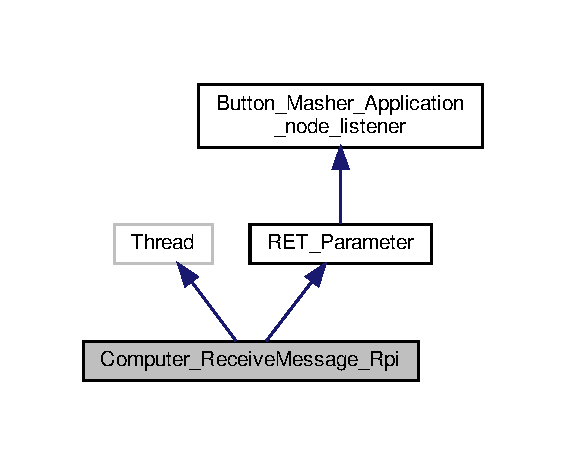
\includegraphics[width=272pt]{classRET__socket_1_1Computer__ReceiveMessage__Rpi__inherit__graph}
\end{center}
\end{figure}


Collaboration diagram for Computer\+\_\+\+Receive\+Message\+\_\+\+Rpi\+:
\nopagebreak
\begin{figure}[H]
\begin{center}
\leavevmode
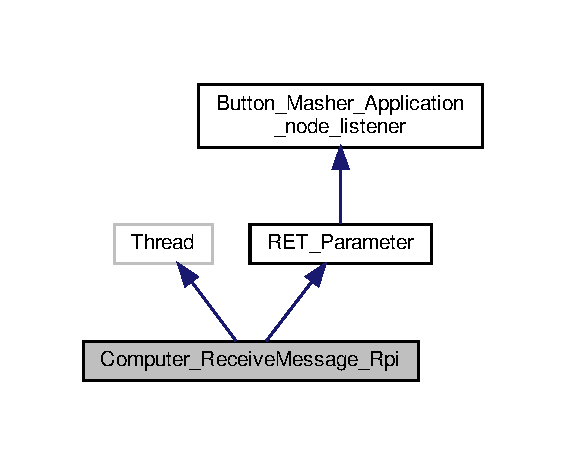
\includegraphics[width=272pt]{classRET__socket_1_1Computer__ReceiveMessage__Rpi__coll__graph}
\end{center}
\end{figure}
\subsection*{Public Member Functions}
\begin{DoxyCompactItemize}
\item 
def \hyperlink{classRET__socket_1_1Computer__ReceiveMessage__Rpi_a1370d57533cdac08e579f9012c0bcd7d}{\+\_\+\+\_\+init\+\_\+\+\_\+} (self, \hyperlink{classRET__socket_1_1Computer__ReceiveMessage__Rpi_a0d71b5c1dcca8d3fee88d6a11d3e2071}{parameter}, \hyperlink{classRET__socket_1_1Computer__ReceiveMessage__Rpi_a10275a078bd1abcbebc206cc5d19e18b}{connection})
\begin{DoxyCompactList}\small\item\em The \hyperlink{classRET__socket_1_1Computer__ReceiveMessage__Rpi}{Computer\+\_\+\+Receive\+Message\+\_\+\+Rpi} class initializer. \end{DoxyCompactList}\item 
def \hyperlink{classRET__socket_1_1Computer__ReceiveMessage__Rpi_ad22709b2e67308af35f55680d5a026e0}{run} (self)
\begin{DoxyCompactList}\small\item\em Retrieves \hyperlink{classRET__socket_1_1Computer__ReceiveMessage__Rpi}{Computer\+\_\+\+Receive\+Message\+\_\+\+Rpi} description. \end{DoxyCompactList}\end{DoxyCompactItemize}
\subsection*{Public Attributes}
\begin{DoxyCompactItemize}
\item 
\hyperlink{classRET__socket_1_1Computer__ReceiveMessage__Rpi_a10275a078bd1abcbebc206cc5d19e18b}{connection}
\item 
\hyperlink{classRET__socket_1_1Computer__ReceiveMessage__Rpi_a0d71b5c1dcca8d3fee88d6a11d3e2071}{parameter}
\end{DoxyCompactItemize}


\subsection{Detailed Description}
The \hyperlink{classRET__socket_1_1Computer__ReceiveMessage__Rpi}{Computer\+\_\+\+Receive\+Message\+\_\+\+Rpi} R\+ET class. 

Provides access to the message sent by the Raspberri Pi. 

\subsection{Constructor \& Destructor Documentation}
\mbox{\Hypertarget{classRET__socket_1_1Computer__ReceiveMessage__Rpi_a1370d57533cdac08e579f9012c0bcd7d}\label{classRET__socket_1_1Computer__ReceiveMessage__Rpi_a1370d57533cdac08e579f9012c0bcd7d}} 
\index{R\+E\+T\+\_\+socket\+::\+Computer\+\_\+\+Receive\+Message\+\_\+\+Rpi@{R\+E\+T\+\_\+socket\+::\+Computer\+\_\+\+Receive\+Message\+\_\+\+Rpi}!\+\_\+\+\_\+init\+\_\+\+\_\+@{\+\_\+\+\_\+init\+\_\+\+\_\+}}
\index{\+\_\+\+\_\+init\+\_\+\+\_\+@{\+\_\+\+\_\+init\+\_\+\+\_\+}!R\+E\+T\+\_\+socket\+::\+Computer\+\_\+\+Receive\+Message\+\_\+\+Rpi@{R\+E\+T\+\_\+socket\+::\+Computer\+\_\+\+Receive\+Message\+\_\+\+Rpi}}
\subsubsection{\texorpdfstring{\+\_\+\+\_\+init\+\_\+\+\_\+()}{\_\_init\_\_()}}
{\footnotesize\ttfamily def \+\_\+\+\_\+init\+\_\+\+\_\+ (\begin{DoxyParamCaption}\item[{}]{self,  }\item[{}]{parameter,  }\item[{}]{connection }\end{DoxyParamCaption})}



The \hyperlink{classRET__socket_1_1Computer__ReceiveMessage__Rpi}{Computer\+\_\+\+Receive\+Message\+\_\+\+Rpi} class initializer. 


\begin{DoxyParams}{Parameters}
{\em parameter} & The parameter we are working with. \\
\hline
{\em connection} & The connection to the socket\textquotesingle{}s server on the Raspberri Pi. \\
\hline
\end{DoxyParams}
\begin{DoxyReturn}{Returns}
An instance of the \hyperlink{classRET__socket_1_1Computer__ReceiveMessage__Rpi}{Computer\+\_\+\+Receive\+Message\+\_\+\+Rpi} class initialized with the specified name. 
\end{DoxyReturn}


\subsection{Member Function Documentation}
\mbox{\Hypertarget{classRET__socket_1_1Computer__ReceiveMessage__Rpi_ad22709b2e67308af35f55680d5a026e0}\label{classRET__socket_1_1Computer__ReceiveMessage__Rpi_ad22709b2e67308af35f55680d5a026e0}} 
\index{R\+E\+T\+\_\+socket\+::\+Computer\+\_\+\+Receive\+Message\+\_\+\+Rpi@{R\+E\+T\+\_\+socket\+::\+Computer\+\_\+\+Receive\+Message\+\_\+\+Rpi}!run@{run}}
\index{run@{run}!R\+E\+T\+\_\+socket\+::\+Computer\+\_\+\+Receive\+Message\+\_\+\+Rpi@{R\+E\+T\+\_\+socket\+::\+Computer\+\_\+\+Receive\+Message\+\_\+\+Rpi}}
\subsubsection{\texorpdfstring{run()}{run()}}
{\footnotesize\ttfamily def run (\begin{DoxyParamCaption}\item[{}]{self }\end{DoxyParamCaption})}



Retrieves \hyperlink{classRET__socket_1_1Computer__ReceiveMessage__Rpi}{Computer\+\_\+\+Receive\+Message\+\_\+\+Rpi} description. 

\begin{DoxyReturn}{Returns}
A thread that runs during the R\+ET. 
\end{DoxyReturn}


\subsection{Member Data Documentation}
\mbox{\Hypertarget{classRET__socket_1_1Computer__ReceiveMessage__Rpi_a10275a078bd1abcbebc206cc5d19e18b}\label{classRET__socket_1_1Computer__ReceiveMessage__Rpi_a10275a078bd1abcbebc206cc5d19e18b}} 
\index{R\+E\+T\+\_\+socket\+::\+Computer\+\_\+\+Receive\+Message\+\_\+\+Rpi@{R\+E\+T\+\_\+socket\+::\+Computer\+\_\+\+Receive\+Message\+\_\+\+Rpi}!connection@{connection}}
\index{connection@{connection}!R\+E\+T\+\_\+socket\+::\+Computer\+\_\+\+Receive\+Message\+\_\+\+Rpi@{R\+E\+T\+\_\+socket\+::\+Computer\+\_\+\+Receive\+Message\+\_\+\+Rpi}}
\subsubsection{\texorpdfstring{connection}{connection}}
{\footnotesize\ttfamily connection}

\mbox{\Hypertarget{classRET__socket_1_1Computer__ReceiveMessage__Rpi_a0d71b5c1dcca8d3fee88d6a11d3e2071}\label{classRET__socket_1_1Computer__ReceiveMessage__Rpi_a0d71b5c1dcca8d3fee88d6a11d3e2071}} 
\index{R\+E\+T\+\_\+socket\+::\+Computer\+\_\+\+Receive\+Message\+\_\+\+Rpi@{R\+E\+T\+\_\+socket\+::\+Computer\+\_\+\+Receive\+Message\+\_\+\+Rpi}!parameter@{parameter}}
\index{parameter@{parameter}!R\+E\+T\+\_\+socket\+::\+Computer\+\_\+\+Receive\+Message\+\_\+\+Rpi@{R\+E\+T\+\_\+socket\+::\+Computer\+\_\+\+Receive\+Message\+\_\+\+Rpi}}
\subsubsection{\texorpdfstring{parameter}{parameter}}
{\footnotesize\ttfamily parameter}



The documentation for this class was generated from the following file\+:\begin{DoxyCompactItemize}
\item 
/home/ret/workspaces/ret/src/ret/scripts/\hyperlink{RET__socket_8py}{R\+E\+T\+\_\+socket.\+py}\end{DoxyCompactItemize}

\hypertarget{classRET__socket_1_1Computer__SendMessage__Rpi}{}\section{Computer\+\_\+\+Send\+Message\+\_\+\+Rpi Class Reference}
\label{classRET__socket_1_1Computer__SendMessage__Rpi}\index{Computer\+\_\+\+Send\+Message\+\_\+\+Rpi@{Computer\+\_\+\+Send\+Message\+\_\+\+Rpi}}


The \hyperlink{classRET__socket_1_1Computer__SendMessage__Rpi}{Computer\+\_\+\+Send\+Message\+\_\+\+Rpi} R\+ET class.  




Inheritance diagram for Computer\+\_\+\+Send\+Message\+\_\+\+Rpi\+:
\nopagebreak
\begin{figure}[H]
\begin{center}
\leavevmode
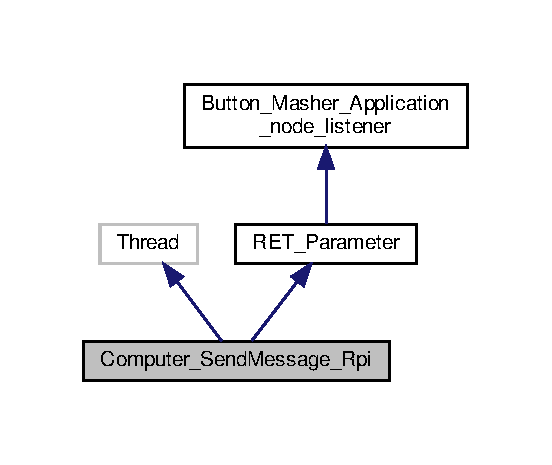
\includegraphics[width=265pt]{classRET__socket_1_1Computer__SendMessage__Rpi__inherit__graph}
\end{center}
\end{figure}


Collaboration diagram for Computer\+\_\+\+Send\+Message\+\_\+\+Rpi\+:
\nopagebreak
\begin{figure}[H]
\begin{center}
\leavevmode
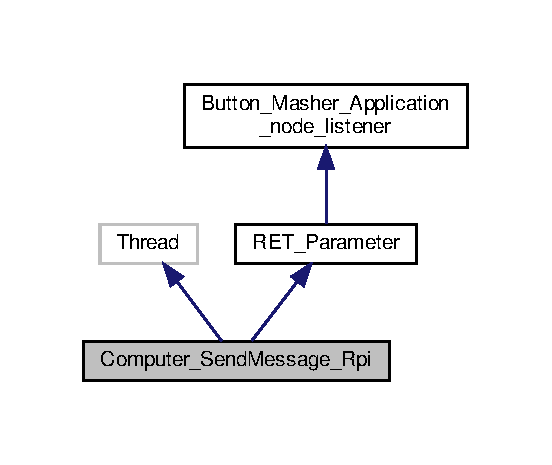
\includegraphics[width=265pt]{classRET__socket_1_1Computer__SendMessage__Rpi__coll__graph}
\end{center}
\end{figure}
\subsection*{Public Member Functions}
\begin{DoxyCompactItemize}
\item 
def \hyperlink{classRET__socket_1_1Computer__SendMessage__Rpi_a1370d57533cdac08e579f9012c0bcd7d}{\+\_\+\+\_\+init\+\_\+\+\_\+} (self, \hyperlink{classRET__socket_1_1Computer__SendMessage__Rpi_a0d71b5c1dcca8d3fee88d6a11d3e2071}{parameter}, \hyperlink{classRET__socket_1_1Computer__SendMessage__Rpi_a10275a078bd1abcbebc206cc5d19e18b}{connection})
\begin{DoxyCompactList}\small\item\em The \hyperlink{classRET__socket_1_1Computer__SendMessage__Rpi}{Computer\+\_\+\+Send\+Message\+\_\+\+Rpi} class initializer. \end{DoxyCompactList}\item 
def \hyperlink{classRET__socket_1_1Computer__SendMessage__Rpi_ad22709b2e67308af35f55680d5a026e0}{run} (self)
\begin{DoxyCompactList}\small\item\em Retrieves \hyperlink{classRET__socket_1_1Computer__SendMessage__Rpi}{Computer\+\_\+\+Send\+Message\+\_\+\+Rpi} description. \end{DoxyCompactList}\item 
def \hyperlink{classRET__socket_1_1Computer__SendMessage__Rpi_aac6ae8e343bc98b533b1384540a840e5}{send\+\_\+message\+\_\+end\+\_\+effector\+\_\+entering\+\_\+button\+\_\+area} (self)
\begin{DoxyCompactList}\small\item\em The \hyperlink{classRET__socket_1_1Computer__SendMessage__Rpi}{Computer\+\_\+\+Send\+Message\+\_\+\+Rpi} class initializer. \end{DoxyCompactList}\item 
def \hyperlink{classRET__socket_1_1Computer__SendMessage__Rpi_a8e7a0eb260cc57a97cf2e0293774d253}{send\+\_\+message\+\_\+end\+\_\+effector\+\_\+leaving\+\_\+button\+\_\+area} (self)
\begin{DoxyCompactList}\small\item\em The \hyperlink{classRET__socket_1_1Computer__SendMessage__Rpi}{Computer\+\_\+\+Send\+Message\+\_\+\+Rpi} class initializer. \end{DoxyCompactList}\end{DoxyCompactItemize}
\subsection*{Public Attributes}
\begin{DoxyCompactItemize}
\item 
\hyperlink{classRET__socket_1_1Computer__SendMessage__Rpi_a10275a078bd1abcbebc206cc5d19e18b}{connection}
\item 
\hyperlink{classRET__socket_1_1Computer__SendMessage__Rpi_a5e1510794909be5332fea558ba24eb78}{list\+\_\+msg\+\_\+send}
\item 
\hyperlink{classRET__socket_1_1Computer__SendMessage__Rpi_a0d71b5c1dcca8d3fee88d6a11d3e2071}{parameter}
\end{DoxyCompactItemize}


\subsection{Detailed Description}
The \hyperlink{classRET__socket_1_1Computer__SendMessage__Rpi}{Computer\+\_\+\+Send\+Message\+\_\+\+Rpi} R\+ET class. 

Provides the possibility to send messages to the Raspberri Pi. 

\subsection{Constructor \& Destructor Documentation}
\mbox{\Hypertarget{classRET__socket_1_1Computer__SendMessage__Rpi_a1370d57533cdac08e579f9012c0bcd7d}\label{classRET__socket_1_1Computer__SendMessage__Rpi_a1370d57533cdac08e579f9012c0bcd7d}} 
\index{R\+E\+T\+\_\+socket\+::\+Computer\+\_\+\+Send\+Message\+\_\+\+Rpi@{R\+E\+T\+\_\+socket\+::\+Computer\+\_\+\+Send\+Message\+\_\+\+Rpi}!\+\_\+\+\_\+init\+\_\+\+\_\+@{\+\_\+\+\_\+init\+\_\+\+\_\+}}
\index{\+\_\+\+\_\+init\+\_\+\+\_\+@{\+\_\+\+\_\+init\+\_\+\+\_\+}!R\+E\+T\+\_\+socket\+::\+Computer\+\_\+\+Send\+Message\+\_\+\+Rpi@{R\+E\+T\+\_\+socket\+::\+Computer\+\_\+\+Send\+Message\+\_\+\+Rpi}}
\subsubsection{\texorpdfstring{\+\_\+\+\_\+init\+\_\+\+\_\+()}{\_\_init\_\_()}}
{\footnotesize\ttfamily def \+\_\+\+\_\+init\+\_\+\+\_\+ (\begin{DoxyParamCaption}\item[{}]{self,  }\item[{}]{parameter,  }\item[{}]{connection }\end{DoxyParamCaption})}



The \hyperlink{classRET__socket_1_1Computer__SendMessage__Rpi}{Computer\+\_\+\+Send\+Message\+\_\+\+Rpi} class initializer. 


\begin{DoxyParams}{Parameters}
{\em parameter} & The parameter we are working with. \\
\hline
{\em connection} & The connection to the socket\textquotesingle{}s server on the Raspberri Pi. \\
\hline
\end{DoxyParams}
\begin{DoxyReturn}{Returns}
An instance of the \hyperlink{classRET__socket_1_1Computer__SendMessage__Rpi}{Computer\+\_\+\+Send\+Message\+\_\+\+Rpi} class initialized with the specified name. 
\end{DoxyReturn}


\subsection{Member Function Documentation}
\mbox{\Hypertarget{classRET__socket_1_1Computer__SendMessage__Rpi_ad22709b2e67308af35f55680d5a026e0}\label{classRET__socket_1_1Computer__SendMessage__Rpi_ad22709b2e67308af35f55680d5a026e0}} 
\index{R\+E\+T\+\_\+socket\+::\+Computer\+\_\+\+Send\+Message\+\_\+\+Rpi@{R\+E\+T\+\_\+socket\+::\+Computer\+\_\+\+Send\+Message\+\_\+\+Rpi}!run@{run}}
\index{run@{run}!R\+E\+T\+\_\+socket\+::\+Computer\+\_\+\+Send\+Message\+\_\+\+Rpi@{R\+E\+T\+\_\+socket\+::\+Computer\+\_\+\+Send\+Message\+\_\+\+Rpi}}
\subsubsection{\texorpdfstring{run()}{run()}}
{\footnotesize\ttfamily def run (\begin{DoxyParamCaption}\item[{}]{self }\end{DoxyParamCaption})}



Retrieves \hyperlink{classRET__socket_1_1Computer__SendMessage__Rpi}{Computer\+\_\+\+Send\+Message\+\_\+\+Rpi} description. 

\begin{DoxyReturn}{Returns}
A thread that runs during the R\+ET. 
\end{DoxyReturn}
\mbox{\Hypertarget{classRET__socket_1_1Computer__SendMessage__Rpi_aac6ae8e343bc98b533b1384540a840e5}\label{classRET__socket_1_1Computer__SendMessage__Rpi_aac6ae8e343bc98b533b1384540a840e5}} 
\index{R\+E\+T\+\_\+socket\+::\+Computer\+\_\+\+Send\+Message\+\_\+\+Rpi@{R\+E\+T\+\_\+socket\+::\+Computer\+\_\+\+Send\+Message\+\_\+\+Rpi}!send\+\_\+message\+\_\+end\+\_\+effector\+\_\+entering\+\_\+button\+\_\+area@{send\+\_\+message\+\_\+end\+\_\+effector\+\_\+entering\+\_\+button\+\_\+area}}
\index{send\+\_\+message\+\_\+end\+\_\+effector\+\_\+entering\+\_\+button\+\_\+area@{send\+\_\+message\+\_\+end\+\_\+effector\+\_\+entering\+\_\+button\+\_\+area}!R\+E\+T\+\_\+socket\+::\+Computer\+\_\+\+Send\+Message\+\_\+\+Rpi@{R\+E\+T\+\_\+socket\+::\+Computer\+\_\+\+Send\+Message\+\_\+\+Rpi}}
\subsubsection{\texorpdfstring{send\+\_\+message\+\_\+end\+\_\+effector\+\_\+entering\+\_\+button\+\_\+area()}{send\_message\_end\_effector\_entering\_button\_area()}}
{\footnotesize\ttfamily def send\+\_\+message\+\_\+end\+\_\+effector\+\_\+entering\+\_\+button\+\_\+area (\begin{DoxyParamCaption}\item[{}]{self }\end{DoxyParamCaption})}



The \hyperlink{classRET__socket_1_1Computer__SendMessage__Rpi}{Computer\+\_\+\+Send\+Message\+\_\+\+Rpi} class initializer. 

\begin{DoxyReturn}{Returns}
The Computer send a message to the Raspberri Pi that we are entering a button\textquotesingle{}s area. 
\end{DoxyReturn}
\mbox{\Hypertarget{classRET__socket_1_1Computer__SendMessage__Rpi_a8e7a0eb260cc57a97cf2e0293774d253}\label{classRET__socket_1_1Computer__SendMessage__Rpi_a8e7a0eb260cc57a97cf2e0293774d253}} 
\index{R\+E\+T\+\_\+socket\+::\+Computer\+\_\+\+Send\+Message\+\_\+\+Rpi@{R\+E\+T\+\_\+socket\+::\+Computer\+\_\+\+Send\+Message\+\_\+\+Rpi}!send\+\_\+message\+\_\+end\+\_\+effector\+\_\+leaving\+\_\+button\+\_\+area@{send\+\_\+message\+\_\+end\+\_\+effector\+\_\+leaving\+\_\+button\+\_\+area}}
\index{send\+\_\+message\+\_\+end\+\_\+effector\+\_\+leaving\+\_\+button\+\_\+area@{send\+\_\+message\+\_\+end\+\_\+effector\+\_\+leaving\+\_\+button\+\_\+area}!R\+E\+T\+\_\+socket\+::\+Computer\+\_\+\+Send\+Message\+\_\+\+Rpi@{R\+E\+T\+\_\+socket\+::\+Computer\+\_\+\+Send\+Message\+\_\+\+Rpi}}
\subsubsection{\texorpdfstring{send\+\_\+message\+\_\+end\+\_\+effector\+\_\+leaving\+\_\+button\+\_\+area()}{send\_message\_end\_effector\_leaving\_button\_area()}}
{\footnotesize\ttfamily def send\+\_\+message\+\_\+end\+\_\+effector\+\_\+leaving\+\_\+button\+\_\+area (\begin{DoxyParamCaption}\item[{}]{self }\end{DoxyParamCaption})}



The \hyperlink{classRET__socket_1_1Computer__SendMessage__Rpi}{Computer\+\_\+\+Send\+Message\+\_\+\+Rpi} class initializer. 

\begin{DoxyReturn}{Returns}
The Computer send a message to the Raspberri Pi that we are leaving a button\textquotesingle{}s area. 
\end{DoxyReturn}


\subsection{Member Data Documentation}
\mbox{\Hypertarget{classRET__socket_1_1Computer__SendMessage__Rpi_a10275a078bd1abcbebc206cc5d19e18b}\label{classRET__socket_1_1Computer__SendMessage__Rpi_a10275a078bd1abcbebc206cc5d19e18b}} 
\index{R\+E\+T\+\_\+socket\+::\+Computer\+\_\+\+Send\+Message\+\_\+\+Rpi@{R\+E\+T\+\_\+socket\+::\+Computer\+\_\+\+Send\+Message\+\_\+\+Rpi}!connection@{connection}}
\index{connection@{connection}!R\+E\+T\+\_\+socket\+::\+Computer\+\_\+\+Send\+Message\+\_\+\+Rpi@{R\+E\+T\+\_\+socket\+::\+Computer\+\_\+\+Send\+Message\+\_\+\+Rpi}}
\subsubsection{\texorpdfstring{connection}{connection}}
{\footnotesize\ttfamily connection}

\mbox{\Hypertarget{classRET__socket_1_1Computer__SendMessage__Rpi_a5e1510794909be5332fea558ba24eb78}\label{classRET__socket_1_1Computer__SendMessage__Rpi_a5e1510794909be5332fea558ba24eb78}} 
\index{R\+E\+T\+\_\+socket\+::\+Computer\+\_\+\+Send\+Message\+\_\+\+Rpi@{R\+E\+T\+\_\+socket\+::\+Computer\+\_\+\+Send\+Message\+\_\+\+Rpi}!list\+\_\+msg\+\_\+send@{list\+\_\+msg\+\_\+send}}
\index{list\+\_\+msg\+\_\+send@{list\+\_\+msg\+\_\+send}!R\+E\+T\+\_\+socket\+::\+Computer\+\_\+\+Send\+Message\+\_\+\+Rpi@{R\+E\+T\+\_\+socket\+::\+Computer\+\_\+\+Send\+Message\+\_\+\+Rpi}}
\subsubsection{\texorpdfstring{list\+\_\+msg\+\_\+send}{list\_msg\_send}}
{\footnotesize\ttfamily list\+\_\+msg\+\_\+send}

\mbox{\Hypertarget{classRET__socket_1_1Computer__SendMessage__Rpi_a0d71b5c1dcca8d3fee88d6a11d3e2071}\label{classRET__socket_1_1Computer__SendMessage__Rpi_a0d71b5c1dcca8d3fee88d6a11d3e2071}} 
\index{R\+E\+T\+\_\+socket\+::\+Computer\+\_\+\+Send\+Message\+\_\+\+Rpi@{R\+E\+T\+\_\+socket\+::\+Computer\+\_\+\+Send\+Message\+\_\+\+Rpi}!parameter@{parameter}}
\index{parameter@{parameter}!R\+E\+T\+\_\+socket\+::\+Computer\+\_\+\+Send\+Message\+\_\+\+Rpi@{R\+E\+T\+\_\+socket\+::\+Computer\+\_\+\+Send\+Message\+\_\+\+Rpi}}
\subsubsection{\texorpdfstring{parameter}{parameter}}
{\footnotesize\ttfamily parameter}



The documentation for this class was generated from the following file\+:\begin{DoxyCompactItemize}
\item 
/home/ret/workspaces/ret/src/ret/scripts/\hyperlink{RET__socket_8py}{R\+E\+T\+\_\+socket.\+py}\end{DoxyCompactItemize}

\hypertarget{classRET__socket_1_1Computer__SocketClient__RET}{}\section{Computer\+\_\+\+Socket\+Client\+\_\+\+R\+ET Class Reference}
\label{classRET__socket_1_1Computer__SocketClient__RET}\index{Computer\+\_\+\+Socket\+Client\+\_\+\+R\+ET@{Computer\+\_\+\+Socket\+Client\+\_\+\+R\+ET}}


The \hyperlink{classRET__socket_1_1Computer__SocketClient__RET}{Computer\+\_\+\+Socket\+Client\+\_\+\+R\+ET} R\+ET class.  




Inheritance diagram for Computer\+\_\+\+Socket\+Client\+\_\+\+R\+ET\+:
\nopagebreak
\begin{figure}[H]
\begin{center}
\leavevmode
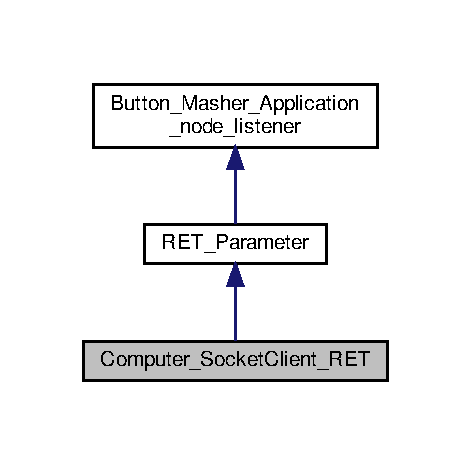
\includegraphics[width=226pt]{classRET__socket_1_1Computer__SocketClient__RET__inherit__graph}
\end{center}
\end{figure}


Collaboration diagram for Computer\+\_\+\+Socket\+Client\+\_\+\+R\+ET\+:
\nopagebreak
\begin{figure}[H]
\begin{center}
\leavevmode
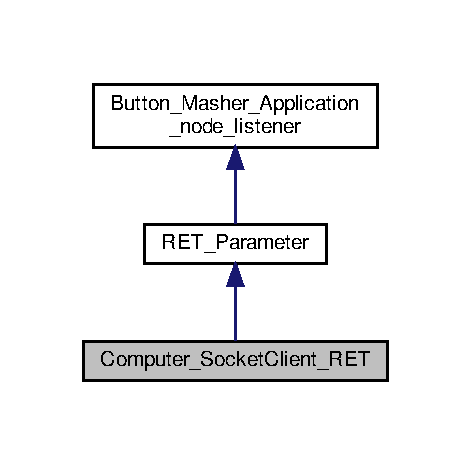
\includegraphics[width=226pt]{classRET__socket_1_1Computer__SocketClient__RET__coll__graph}
\end{center}
\end{figure}
\subsection*{Public Member Functions}
\begin{DoxyCompactItemize}
\item 
def \hyperlink{classRET__socket_1_1Computer__SocketClient__RET_a297f3b1ee42e9ff40c0ec84bb5996ea5}{\+\_\+\+\_\+init\+\_\+\+\_\+} (self, \hyperlink{classRET__socket_1_1Computer__SocketClient__RET_a0d71b5c1dcca8d3fee88d6a11d3e2071}{parameter})
\begin{DoxyCompactList}\small\item\em The \hyperlink{classRET__socket_1_1Computer__SendMessage__Rpi}{Computer\+\_\+\+Send\+Message\+\_\+\+Rpi} class initializer. \end{DoxyCompactList}\end{DoxyCompactItemize}
\subsection*{Public Attributes}
\begin{DoxyCompactItemize}
\item 
\hyperlink{classRET__socket_1_1Computer__SocketClient__RET_a10275a078bd1abcbebc206cc5d19e18b}{connection}
\item 
\hyperlink{classRET__socket_1_1Computer__SocketClient__RET_a0d71b5c1dcca8d3fee88d6a11d3e2071}{parameter}
\end{DoxyCompactItemize}


\subsection{Detailed Description}
The \hyperlink{classRET__socket_1_1Computer__SocketClient__RET}{Computer\+\_\+\+Socket\+Client\+\_\+\+R\+ET} R\+ET class. 

Provides a socket\textquotesingle{}s client. 

\subsection{Constructor \& Destructor Documentation}
\mbox{\Hypertarget{classRET__socket_1_1Computer__SocketClient__RET_a297f3b1ee42e9ff40c0ec84bb5996ea5}\label{classRET__socket_1_1Computer__SocketClient__RET_a297f3b1ee42e9ff40c0ec84bb5996ea5}} 
\index{R\+E\+T\+\_\+socket\+::\+Computer\+\_\+\+Socket\+Client\+\_\+\+R\+ET@{R\+E\+T\+\_\+socket\+::\+Computer\+\_\+\+Socket\+Client\+\_\+\+R\+ET}!\+\_\+\+\_\+init\+\_\+\+\_\+@{\+\_\+\+\_\+init\+\_\+\+\_\+}}
\index{\+\_\+\+\_\+init\+\_\+\+\_\+@{\+\_\+\+\_\+init\+\_\+\+\_\+}!R\+E\+T\+\_\+socket\+::\+Computer\+\_\+\+Socket\+Client\+\_\+\+R\+ET@{R\+E\+T\+\_\+socket\+::\+Computer\+\_\+\+Socket\+Client\+\_\+\+R\+ET}}
\subsubsection{\texorpdfstring{\+\_\+\+\_\+init\+\_\+\+\_\+()}{\_\_init\_\_()}}
{\footnotesize\ttfamily def \+\_\+\+\_\+init\+\_\+\+\_\+ (\begin{DoxyParamCaption}\item[{}]{self,  }\item[{}]{parameter }\end{DoxyParamCaption})}



The \hyperlink{classRET__socket_1_1Computer__SendMessage__Rpi}{Computer\+\_\+\+Send\+Message\+\_\+\+Rpi} class initializer. 


\begin{DoxyParams}{Parameters}
{\em parameter} & The parameter we are working with. \\
\hline
\end{DoxyParams}
\begin{DoxyReturn}{Returns}
Two thread that communicates from the computer to the Raspberri Pi. 
\end{DoxyReturn}


\subsection{Member Data Documentation}
\mbox{\Hypertarget{classRET__socket_1_1Computer__SocketClient__RET_a10275a078bd1abcbebc206cc5d19e18b}\label{classRET__socket_1_1Computer__SocketClient__RET_a10275a078bd1abcbebc206cc5d19e18b}} 
\index{R\+E\+T\+\_\+socket\+::\+Computer\+\_\+\+Socket\+Client\+\_\+\+R\+ET@{R\+E\+T\+\_\+socket\+::\+Computer\+\_\+\+Socket\+Client\+\_\+\+R\+ET}!connection@{connection}}
\index{connection@{connection}!R\+E\+T\+\_\+socket\+::\+Computer\+\_\+\+Socket\+Client\+\_\+\+R\+ET@{R\+E\+T\+\_\+socket\+::\+Computer\+\_\+\+Socket\+Client\+\_\+\+R\+ET}}
\subsubsection{\texorpdfstring{connection}{connection}}
{\footnotesize\ttfamily connection}

\mbox{\Hypertarget{classRET__socket_1_1Computer__SocketClient__RET_a0d71b5c1dcca8d3fee88d6a11d3e2071}\label{classRET__socket_1_1Computer__SocketClient__RET_a0d71b5c1dcca8d3fee88d6a11d3e2071}} 
\index{R\+E\+T\+\_\+socket\+::\+Computer\+\_\+\+Socket\+Client\+\_\+\+R\+ET@{R\+E\+T\+\_\+socket\+::\+Computer\+\_\+\+Socket\+Client\+\_\+\+R\+ET}!parameter@{parameter}}
\index{parameter@{parameter}!R\+E\+T\+\_\+socket\+::\+Computer\+\_\+\+Socket\+Client\+\_\+\+R\+ET@{R\+E\+T\+\_\+socket\+::\+Computer\+\_\+\+Socket\+Client\+\_\+\+R\+ET}}
\subsubsection{\texorpdfstring{parameter}{parameter}}
{\footnotesize\ttfamily parameter}



The documentation for this class was generated from the following file\+:\begin{DoxyCompactItemize}
\item 
/home/ret/workspaces/ret/src/ret/scripts/\hyperlink{RET__socket_8py}{R\+E\+T\+\_\+socket.\+py}\end{DoxyCompactItemize}

\hypertarget{classRET__data__processing_1_1RET__data__processing}{}\section{R\+E\+T\+\_\+data\+\_\+processing Class Reference}
\label{classRET__data__processing_1_1RET__data__processing}\index{R\+E\+T\+\_\+data\+\_\+processing@{R\+E\+T\+\_\+data\+\_\+processing}}


The \hyperlink{classRET__data__processing_1_1RET__data__processing}{R\+E\+T\+\_\+data\+\_\+processing} class.  




Inheritance diagram for R\+E\+T\+\_\+data\+\_\+processing\+:
\nopagebreak
\begin{figure}[H]
\begin{center}
\leavevmode
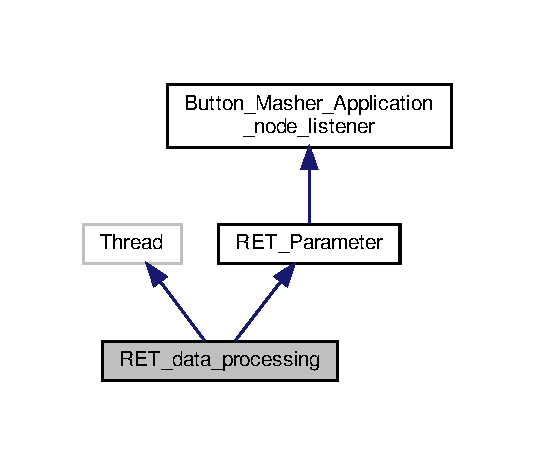
\includegraphics[width=257pt]{classRET__data__processing_1_1RET__data__processing__inherit__graph}
\end{center}
\end{figure}


Collaboration diagram for R\+E\+T\+\_\+data\+\_\+processing\+:
\nopagebreak
\begin{figure}[H]
\begin{center}
\leavevmode
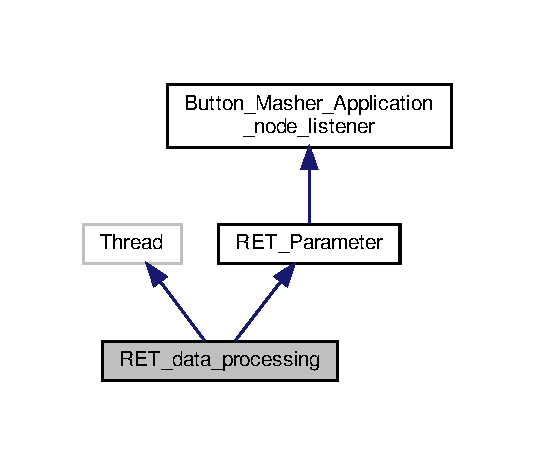
\includegraphics[width=257pt]{classRET__data__processing_1_1RET__data__processing__coll__graph}
\end{center}
\end{figure}
\subsection*{Public Member Functions}
\begin{DoxyCompactItemize}
\item 
def \hyperlink{classRET__data__processing_1_1RET__data__processing_a297f3b1ee42e9ff40c0ec84bb5996ea5}{\+\_\+\+\_\+init\+\_\+\+\_\+} (self, \hyperlink{classRET__data__processing_1_1RET__data__processing_a0d71b5c1dcca8d3fee88d6a11d3e2071}{parameter})
\begin{DoxyCompactList}\small\item\em The \hyperlink{classRET__data__processing_1_1RET__data__processing}{R\+E\+T\+\_\+data\+\_\+processing} class initializer. \end{DoxyCompactList}\item 
def \hyperlink{classRET__data__processing_1_1RET__data__processing_a33b438266e6f03807f16bd4792855730}{end\+\_\+effector\+\_\+inside\+\_\+\+Btn\+\_\+area} (self)
\begin{DoxyCompactList}\small\item\em Retrieves the end effector cartesian position description. \end{DoxyCompactList}\item 
def \hyperlink{classRET__data__processing_1_1RET__data__processing_a5b693dc8f5167e8338541cc72ed583dc}{end\+\_\+effector\+\_\+outside\+\_\+\+Btn\+\_\+area} (self)
\begin{DoxyCompactList}\small\item\em Retrieves the end effector cartesian position description. \end{DoxyCompactList}\item 
def \hyperlink{classRET__data__processing_1_1RET__data__processing_af0d2380cd9fe71bf71ab9b25903cebc2}{process\+\_\+time\+\_\+\+Btn\+\_\+pressed} (self)
\begin{DoxyCompactList}\small\item\em Retrieves the time the button where pressed detected by the Raspberri Pi. \end{DoxyCompactList}\item 
def \hyperlink{classRET__data__processing_1_1RET__data__processing_ad22709b2e67308af35f55680d5a026e0}{run} (self)
\begin{DoxyCompactList}\small\item\em Retrieves \hyperlink{classRET__data__processing_1_1RET__data__processing}{R\+E\+T\+\_\+data\+\_\+processing} class. \end{DoxyCompactList}\item 
def \hyperlink{classRET__data__processing_1_1RET__data__processing_a53cc9f2963d8567e8f2be4663fbe2d92}{write\+\_\+into\+\_\+csv\+\_\+db} (self)
\begin{DoxyCompactList}\small\item\em Retrieves the csv logfile. \end{DoxyCompactList}\item 
def \hyperlink{classRET__data__processing_1_1RET__data__processing_a8edbf01e68042082bbe5bc8c967f710e}{write\+\_\+into\+\_\+influxdb} (self, \hyperlink{classRET__data__processing_1_1RET__data__processing_ad5bc32b75da65fe60067f501a4bb6665}{client})
\begin{DoxyCompactList}\small\item\em Retrieves the time the button where pressed detected by the Raspberri Pi. \end{DoxyCompactList}\item 
def \hyperlink{classRET__data__processing_1_1RET__data__processing_a7ced1bb55d644f56ba40295ffed86c92}{write\+\_\+json\+\_\+influxdb\+\_\+additional\+\_\+information} (self, \hyperlink{classRET__data__processing_1_1RET__data__processing_ad5bc32b75da65fe60067f501a4bb6665}{client})
\begin{DoxyCompactList}\small\item\em Retrieves additional data. \end{DoxyCompactList}\item 
def \hyperlink{classRET__data__processing_1_1RET__data__processing_abb33542be6fa47a380328883d58d1c79}{write\+\_\+json\+\_\+influxdb\+\_\+\+R\+ET} (self, \hyperlink{classRET__data__processing_1_1RET__data__processing_ad5bc32b75da65fe60067f501a4bb6665}{client})
\end{DoxyCompactItemize}
\subsection*{Public Attributes}
\begin{DoxyCompactItemize}
\item 
\hyperlink{classRET__data__processing_1_1RET__data__processing_ad5bc32b75da65fe60067f501a4bb6665}{client}
\begin{DoxyCompactList}\small\item\em argument for Influxdb \end{DoxyCompactList}\item 
\hyperlink{classRET__data__processing_1_1RET__data__processing_af140727efa8da9cde0e592a61407d62f}{inside\+\_\+one\+\_\+button\+\_\+area}
\begin{DoxyCompactList}\small\item\em settle arguments to deal only with one Btn at the time, we cannot process every button of the list anytime \end{DoxyCompactList}\item 
\hyperlink{classRET__data__processing_1_1RET__data__processing_acbbf8e6a1d50b851956b602b4b62407d}{len\+\_\+list\+\_\+buttons\+\_\+area}
\begin{DoxyCompactList}\small\item\em add a parameter that determine which button we have to work on, instead of working on every button of the list anytime \end{DoxyCompactList}\item 
\hyperlink{classRET__data__processing_1_1RET__data__processing_a0d71b5c1dcca8d3fee88d6a11d3e2071}{parameter}
\item 
\hyperlink{classRET__data__processing_1_1RET__data__processing_ae694f95e6ad7f44763d44d68466b8011}{process\+\_\+data}
\item 
\hyperlink{classRET__data__processing_1_1RET__data__processing_a96204c1a4417d5a3a980521f8a66a1fa}{working\+\_\+on\+\_\+button}
\end{DoxyCompactItemize}


\subsection{Detailed Description}
The \hyperlink{classRET__data__processing_1_1RET__data__processing}{R\+E\+T\+\_\+data\+\_\+processing} class. 

Provides access to the processing of the data in the R\+ET. 

\subsection{Constructor \& Destructor Documentation}
\mbox{\Hypertarget{classRET__data__processing_1_1RET__data__processing_a297f3b1ee42e9ff40c0ec84bb5996ea5}\label{classRET__data__processing_1_1RET__data__processing_a297f3b1ee42e9ff40c0ec84bb5996ea5}} 
\index{R\+E\+T\+\_\+data\+\_\+processing\+::\+R\+E\+T\+\_\+data\+\_\+processing@{R\+E\+T\+\_\+data\+\_\+processing\+::\+R\+E\+T\+\_\+data\+\_\+processing}!\+\_\+\+\_\+init\+\_\+\+\_\+@{\+\_\+\+\_\+init\+\_\+\+\_\+}}
\index{\+\_\+\+\_\+init\+\_\+\+\_\+@{\+\_\+\+\_\+init\+\_\+\+\_\+}!R\+E\+T\+\_\+data\+\_\+processing\+::\+R\+E\+T\+\_\+data\+\_\+processing@{R\+E\+T\+\_\+data\+\_\+processing\+::\+R\+E\+T\+\_\+data\+\_\+processing}}
\subsubsection{\texorpdfstring{\+\_\+\+\_\+init\+\_\+\+\_\+()}{\_\_init\_\_()}}
{\footnotesize\ttfamily def \+\_\+\+\_\+init\+\_\+\+\_\+ (\begin{DoxyParamCaption}\item[{}]{self,  }\item[{}]{parameter }\end{DoxyParamCaption})}



The \hyperlink{classRET__data__processing_1_1RET__data__processing}{R\+E\+T\+\_\+data\+\_\+processing} class initializer. 


\begin{DoxyParams}{Parameters}
{\em parameter} & The parameter of the R\+ET we are processing that includes the data we work with. \\
\hline
\end{DoxyParams}
\begin{DoxyReturn}{Returns}
A thread instance that process the data while the R\+ET is running. 
\end{DoxyReturn}


\subsection{Member Function Documentation}
\mbox{\Hypertarget{classRET__data__processing_1_1RET__data__processing_a33b438266e6f03807f16bd4792855730}\label{classRET__data__processing_1_1RET__data__processing_a33b438266e6f03807f16bd4792855730}} 
\index{R\+E\+T\+\_\+data\+\_\+processing\+::\+R\+E\+T\+\_\+data\+\_\+processing@{R\+E\+T\+\_\+data\+\_\+processing\+::\+R\+E\+T\+\_\+data\+\_\+processing}!end\+\_\+effector\+\_\+inside\+\_\+\+Btn\+\_\+area@{end\+\_\+effector\+\_\+inside\+\_\+\+Btn\+\_\+area}}
\index{end\+\_\+effector\+\_\+inside\+\_\+\+Btn\+\_\+area@{end\+\_\+effector\+\_\+inside\+\_\+\+Btn\+\_\+area}!R\+E\+T\+\_\+data\+\_\+processing\+::\+R\+E\+T\+\_\+data\+\_\+processing@{R\+E\+T\+\_\+data\+\_\+processing\+::\+R\+E\+T\+\_\+data\+\_\+processing}}
\subsubsection{\texorpdfstring{end\+\_\+effector\+\_\+inside\+\_\+\+Btn\+\_\+area()}{end\_effector\_inside\_Btn\_area()}}
{\footnotesize\ttfamily def end\+\_\+effector\+\_\+inside\+\_\+\+Btn\+\_\+area (\begin{DoxyParamCaption}\item[{}]{self }\end{DoxyParamCaption})}



Retrieves the end effector cartesian position description. 

\begin{DoxyReturn}{Returns}
The event of the end effector entering a button\textquotesingle{}s area. 
\end{DoxyReturn}
\mbox{\Hypertarget{classRET__data__processing_1_1RET__data__processing_a5b693dc8f5167e8338541cc72ed583dc}\label{classRET__data__processing_1_1RET__data__processing_a5b693dc8f5167e8338541cc72ed583dc}} 
\index{R\+E\+T\+\_\+data\+\_\+processing\+::\+R\+E\+T\+\_\+data\+\_\+processing@{R\+E\+T\+\_\+data\+\_\+processing\+::\+R\+E\+T\+\_\+data\+\_\+processing}!end\+\_\+effector\+\_\+outside\+\_\+\+Btn\+\_\+area@{end\+\_\+effector\+\_\+outside\+\_\+\+Btn\+\_\+area}}
\index{end\+\_\+effector\+\_\+outside\+\_\+\+Btn\+\_\+area@{end\+\_\+effector\+\_\+outside\+\_\+\+Btn\+\_\+area}!R\+E\+T\+\_\+data\+\_\+processing\+::\+R\+E\+T\+\_\+data\+\_\+processing@{R\+E\+T\+\_\+data\+\_\+processing\+::\+R\+E\+T\+\_\+data\+\_\+processing}}
\subsubsection{\texorpdfstring{end\+\_\+effector\+\_\+outside\+\_\+\+Btn\+\_\+area()}{end\_effector\_outside\_Btn\_area()}}
{\footnotesize\ttfamily def end\+\_\+effector\+\_\+outside\+\_\+\+Btn\+\_\+area (\begin{DoxyParamCaption}\item[{}]{self }\end{DoxyParamCaption})}



Retrieves the end effector cartesian position description. 

\begin{DoxyReturn}{Returns}
The event of the end effector leaving a button\textquotesingle{}s area. 
\end{DoxyReturn}
\mbox{\Hypertarget{classRET__data__processing_1_1RET__data__processing_af0d2380cd9fe71bf71ab9b25903cebc2}\label{classRET__data__processing_1_1RET__data__processing_af0d2380cd9fe71bf71ab9b25903cebc2}} 
\index{R\+E\+T\+\_\+data\+\_\+processing\+::\+R\+E\+T\+\_\+data\+\_\+processing@{R\+E\+T\+\_\+data\+\_\+processing\+::\+R\+E\+T\+\_\+data\+\_\+processing}!process\+\_\+time\+\_\+\+Btn\+\_\+pressed@{process\+\_\+time\+\_\+\+Btn\+\_\+pressed}}
\index{process\+\_\+time\+\_\+\+Btn\+\_\+pressed@{process\+\_\+time\+\_\+\+Btn\+\_\+pressed}!R\+E\+T\+\_\+data\+\_\+processing\+::\+R\+E\+T\+\_\+data\+\_\+processing@{R\+E\+T\+\_\+data\+\_\+processing\+::\+R\+E\+T\+\_\+data\+\_\+processing}}
\subsubsection{\texorpdfstring{process\+\_\+time\+\_\+\+Btn\+\_\+pressed()}{process\_time\_Btn\_pressed()}}
{\footnotesize\ttfamily def process\+\_\+time\+\_\+\+Btn\+\_\+pressed (\begin{DoxyParamCaption}\item[{}]{self }\end{DoxyParamCaption})}



Retrieves the time the button where pressed detected by the Raspberri Pi. 

\begin{DoxyReturn}{Returns}
The event of the time the button pressed inside the interval of time the button is entering and leaving the button area or not. 
\end{DoxyReturn}
\mbox{\Hypertarget{classRET__data__processing_1_1RET__data__processing_ad22709b2e67308af35f55680d5a026e0}\label{classRET__data__processing_1_1RET__data__processing_ad22709b2e67308af35f55680d5a026e0}} 
\index{R\+E\+T\+\_\+data\+\_\+processing\+::\+R\+E\+T\+\_\+data\+\_\+processing@{R\+E\+T\+\_\+data\+\_\+processing\+::\+R\+E\+T\+\_\+data\+\_\+processing}!run@{run}}
\index{run@{run}!R\+E\+T\+\_\+data\+\_\+processing\+::\+R\+E\+T\+\_\+data\+\_\+processing@{R\+E\+T\+\_\+data\+\_\+processing\+::\+R\+E\+T\+\_\+data\+\_\+processing}}
\subsubsection{\texorpdfstring{run()}{run()}}
{\footnotesize\ttfamily def run (\begin{DoxyParamCaption}\item[{}]{self }\end{DoxyParamCaption})}



Retrieves \hyperlink{classRET__data__processing_1_1RET__data__processing}{R\+E\+T\+\_\+data\+\_\+processing} class. 

\begin{DoxyReturn}{Returns}
Launch the thread that processes the data. 
\end{DoxyReturn}
\mbox{\Hypertarget{classRET__data__processing_1_1RET__data__processing_a53cc9f2963d8567e8f2be4663fbe2d92}\label{classRET__data__processing_1_1RET__data__processing_a53cc9f2963d8567e8f2be4663fbe2d92}} 
\index{R\+E\+T\+\_\+data\+\_\+processing\+::\+R\+E\+T\+\_\+data\+\_\+processing@{R\+E\+T\+\_\+data\+\_\+processing\+::\+R\+E\+T\+\_\+data\+\_\+processing}!write\+\_\+into\+\_\+csv\+\_\+db@{write\+\_\+into\+\_\+csv\+\_\+db}}
\index{write\+\_\+into\+\_\+csv\+\_\+db@{write\+\_\+into\+\_\+csv\+\_\+db}!R\+E\+T\+\_\+data\+\_\+processing\+::\+R\+E\+T\+\_\+data\+\_\+processing@{R\+E\+T\+\_\+data\+\_\+processing\+::\+R\+E\+T\+\_\+data\+\_\+processing}}
\subsubsection{\texorpdfstring{write\+\_\+into\+\_\+csv\+\_\+db()}{write\_into\_csv\_db()}}
{\footnotesize\ttfamily def write\+\_\+into\+\_\+csv\+\_\+db (\begin{DoxyParamCaption}\item[{}]{self }\end{DoxyParamCaption})}



Retrieves the csv logfile. 

\begin{DoxyReturn}{Returns}
Write the R\+ET data in the Influxdb. 
\end{DoxyReturn}
\mbox{\Hypertarget{classRET__data__processing_1_1RET__data__processing_a8edbf01e68042082bbe5bc8c967f710e}\label{classRET__data__processing_1_1RET__data__processing_a8edbf01e68042082bbe5bc8c967f710e}} 
\index{R\+E\+T\+\_\+data\+\_\+processing\+::\+R\+E\+T\+\_\+data\+\_\+processing@{R\+E\+T\+\_\+data\+\_\+processing\+::\+R\+E\+T\+\_\+data\+\_\+processing}!write\+\_\+into\+\_\+influxdb@{write\+\_\+into\+\_\+influxdb}}
\index{write\+\_\+into\+\_\+influxdb@{write\+\_\+into\+\_\+influxdb}!R\+E\+T\+\_\+data\+\_\+processing\+::\+R\+E\+T\+\_\+data\+\_\+processing@{R\+E\+T\+\_\+data\+\_\+processing\+::\+R\+E\+T\+\_\+data\+\_\+processing}}
\subsubsection{\texorpdfstring{write\+\_\+into\+\_\+influxdb()}{write\_into\_influxdb()}}
{\footnotesize\ttfamily def write\+\_\+into\+\_\+influxdb (\begin{DoxyParamCaption}\item[{}]{self,  }\item[{}]{client }\end{DoxyParamCaption})}



Retrieves the time the button where pressed detected by the Raspberri Pi. 

client The influxdb databases we want to log the data in. \begin{DoxyReturn}{Returns}
Write the event of the button pressing inside the time interval in the Influxdb. 
\end{DoxyReturn}
\mbox{\Hypertarget{classRET__data__processing_1_1RET__data__processing_a7ced1bb55d644f56ba40295ffed86c92}\label{classRET__data__processing_1_1RET__data__processing_a7ced1bb55d644f56ba40295ffed86c92}} 
\index{R\+E\+T\+\_\+data\+\_\+processing\+::\+R\+E\+T\+\_\+data\+\_\+processing@{R\+E\+T\+\_\+data\+\_\+processing\+::\+R\+E\+T\+\_\+data\+\_\+processing}!write\+\_\+json\+\_\+influxdb\+\_\+additional\+\_\+information@{write\+\_\+json\+\_\+influxdb\+\_\+additional\+\_\+information}}
\index{write\+\_\+json\+\_\+influxdb\+\_\+additional\+\_\+information@{write\+\_\+json\+\_\+influxdb\+\_\+additional\+\_\+information}!R\+E\+T\+\_\+data\+\_\+processing\+::\+R\+E\+T\+\_\+data\+\_\+processing@{R\+E\+T\+\_\+data\+\_\+processing\+::\+R\+E\+T\+\_\+data\+\_\+processing}}
\subsubsection{\texorpdfstring{write\+\_\+json\+\_\+influxdb\+\_\+additional\+\_\+information()}{write\_json\_influxdb\_additional\_information()}}
{\footnotesize\ttfamily def write\+\_\+json\+\_\+influxdb\+\_\+additional\+\_\+information (\begin{DoxyParamCaption}\item[{}]{self,  }\item[{}]{client }\end{DoxyParamCaption})}



Retrieves additional data. 

client The influxdb databases we want to log the data in. \begin{DoxyReturn}{Returns}
Write the additional data in the Influxdb. 
\end{DoxyReturn}
\mbox{\Hypertarget{classRET__data__processing_1_1RET__data__processing_abb33542be6fa47a380328883d58d1c79}\label{classRET__data__processing_1_1RET__data__processing_abb33542be6fa47a380328883d58d1c79}} 
\index{R\+E\+T\+\_\+data\+\_\+processing\+::\+R\+E\+T\+\_\+data\+\_\+processing@{R\+E\+T\+\_\+data\+\_\+processing\+::\+R\+E\+T\+\_\+data\+\_\+processing}!write\+\_\+json\+\_\+influxdb\+\_\+\+R\+ET@{write\+\_\+json\+\_\+influxdb\+\_\+\+R\+ET}}
\index{write\+\_\+json\+\_\+influxdb\+\_\+\+R\+ET@{write\+\_\+json\+\_\+influxdb\+\_\+\+R\+ET}!R\+E\+T\+\_\+data\+\_\+processing\+::\+R\+E\+T\+\_\+data\+\_\+processing@{R\+E\+T\+\_\+data\+\_\+processing\+::\+R\+E\+T\+\_\+data\+\_\+processing}}
\subsubsection{\texorpdfstring{write\+\_\+json\+\_\+influxdb\+\_\+\+R\+E\+T()}{write\_json\_influxdb\_RET()}}
{\footnotesize\ttfamily def write\+\_\+json\+\_\+influxdb\+\_\+\+R\+ET (\begin{DoxyParamCaption}\item[{}]{self,  }\item[{}]{client }\end{DoxyParamCaption})}



\subsection{Member Data Documentation}
\mbox{\Hypertarget{classRET__data__processing_1_1RET__data__processing_ad5bc32b75da65fe60067f501a4bb6665}\label{classRET__data__processing_1_1RET__data__processing_ad5bc32b75da65fe60067f501a4bb6665}} 
\index{R\+E\+T\+\_\+data\+\_\+processing\+::\+R\+E\+T\+\_\+data\+\_\+processing@{R\+E\+T\+\_\+data\+\_\+processing\+::\+R\+E\+T\+\_\+data\+\_\+processing}!client@{client}}
\index{client@{client}!R\+E\+T\+\_\+data\+\_\+processing\+::\+R\+E\+T\+\_\+data\+\_\+processing@{R\+E\+T\+\_\+data\+\_\+processing\+::\+R\+E\+T\+\_\+data\+\_\+processing}}
\subsubsection{\texorpdfstring{client}{client}}
{\footnotesize\ttfamily client}



argument for Influxdb 

\mbox{\Hypertarget{classRET__data__processing_1_1RET__data__processing_af140727efa8da9cde0e592a61407d62f}\label{classRET__data__processing_1_1RET__data__processing_af140727efa8da9cde0e592a61407d62f}} 
\index{R\+E\+T\+\_\+data\+\_\+processing\+::\+R\+E\+T\+\_\+data\+\_\+processing@{R\+E\+T\+\_\+data\+\_\+processing\+::\+R\+E\+T\+\_\+data\+\_\+processing}!inside\+\_\+one\+\_\+button\+\_\+area@{inside\+\_\+one\+\_\+button\+\_\+area}}
\index{inside\+\_\+one\+\_\+button\+\_\+area@{inside\+\_\+one\+\_\+button\+\_\+area}!R\+E\+T\+\_\+data\+\_\+processing\+::\+R\+E\+T\+\_\+data\+\_\+processing@{R\+E\+T\+\_\+data\+\_\+processing\+::\+R\+E\+T\+\_\+data\+\_\+processing}}
\subsubsection{\texorpdfstring{inside\+\_\+one\+\_\+button\+\_\+area}{inside\_one\_button\_area}}
{\footnotesize\ttfamily inside\+\_\+one\+\_\+button\+\_\+area}



settle arguments to deal only with one Btn at the time, we cannot process every button of the list anytime 

\mbox{\Hypertarget{classRET__data__processing_1_1RET__data__processing_acbbf8e6a1d50b851956b602b4b62407d}\label{classRET__data__processing_1_1RET__data__processing_acbbf8e6a1d50b851956b602b4b62407d}} 
\index{R\+E\+T\+\_\+data\+\_\+processing\+::\+R\+E\+T\+\_\+data\+\_\+processing@{R\+E\+T\+\_\+data\+\_\+processing\+::\+R\+E\+T\+\_\+data\+\_\+processing}!len\+\_\+list\+\_\+buttons\+\_\+area@{len\+\_\+list\+\_\+buttons\+\_\+area}}
\index{len\+\_\+list\+\_\+buttons\+\_\+area@{len\+\_\+list\+\_\+buttons\+\_\+area}!R\+E\+T\+\_\+data\+\_\+processing\+::\+R\+E\+T\+\_\+data\+\_\+processing@{R\+E\+T\+\_\+data\+\_\+processing\+::\+R\+E\+T\+\_\+data\+\_\+processing}}
\subsubsection{\texorpdfstring{len\+\_\+list\+\_\+buttons\+\_\+area}{len\_list\_buttons\_area}}
{\footnotesize\ttfamily len\+\_\+list\+\_\+buttons\+\_\+area}



add a parameter that determine which button we have to work on, instead of working on every button of the list anytime 

\mbox{\Hypertarget{classRET__data__processing_1_1RET__data__processing_a0d71b5c1dcca8d3fee88d6a11d3e2071}\label{classRET__data__processing_1_1RET__data__processing_a0d71b5c1dcca8d3fee88d6a11d3e2071}} 
\index{R\+E\+T\+\_\+data\+\_\+processing\+::\+R\+E\+T\+\_\+data\+\_\+processing@{R\+E\+T\+\_\+data\+\_\+processing\+::\+R\+E\+T\+\_\+data\+\_\+processing}!parameter@{parameter}}
\index{parameter@{parameter}!R\+E\+T\+\_\+data\+\_\+processing\+::\+R\+E\+T\+\_\+data\+\_\+processing@{R\+E\+T\+\_\+data\+\_\+processing\+::\+R\+E\+T\+\_\+data\+\_\+processing}}
\subsubsection{\texorpdfstring{parameter}{parameter}}
{\footnotesize\ttfamily parameter}

\mbox{\Hypertarget{classRET__data__processing_1_1RET__data__processing_ae694f95e6ad7f44763d44d68466b8011}\label{classRET__data__processing_1_1RET__data__processing_ae694f95e6ad7f44763d44d68466b8011}} 
\index{R\+E\+T\+\_\+data\+\_\+processing\+::\+R\+E\+T\+\_\+data\+\_\+processing@{R\+E\+T\+\_\+data\+\_\+processing\+::\+R\+E\+T\+\_\+data\+\_\+processing}!process\+\_\+data@{process\+\_\+data}}
\index{process\+\_\+data@{process\+\_\+data}!R\+E\+T\+\_\+data\+\_\+processing\+::\+R\+E\+T\+\_\+data\+\_\+processing@{R\+E\+T\+\_\+data\+\_\+processing\+::\+R\+E\+T\+\_\+data\+\_\+processing}}
\subsubsection{\texorpdfstring{process\+\_\+data}{process\_data}}
{\footnotesize\ttfamily process\+\_\+data}

\mbox{\Hypertarget{classRET__data__processing_1_1RET__data__processing_a96204c1a4417d5a3a980521f8a66a1fa}\label{classRET__data__processing_1_1RET__data__processing_a96204c1a4417d5a3a980521f8a66a1fa}} 
\index{R\+E\+T\+\_\+data\+\_\+processing\+::\+R\+E\+T\+\_\+data\+\_\+processing@{R\+E\+T\+\_\+data\+\_\+processing\+::\+R\+E\+T\+\_\+data\+\_\+processing}!working\+\_\+on\+\_\+button@{working\+\_\+on\+\_\+button}}
\index{working\+\_\+on\+\_\+button@{working\+\_\+on\+\_\+button}!R\+E\+T\+\_\+data\+\_\+processing\+::\+R\+E\+T\+\_\+data\+\_\+processing@{R\+E\+T\+\_\+data\+\_\+processing\+::\+R\+E\+T\+\_\+data\+\_\+processing}}
\subsubsection{\texorpdfstring{working\+\_\+on\+\_\+button}{working\_on\_button}}
{\footnotesize\ttfamily working\+\_\+on\+\_\+button}



The documentation for this class was generated from the following file\+:\begin{DoxyCompactItemize}
\item 
/home/ret/workspaces/ret/src/ret/scripts/\hyperlink{RET__data__processing_8py}{R\+E\+T\+\_\+data\+\_\+processing.\+py}\end{DoxyCompactItemize}

\hypertarget{classRET__Parameter_1_1RET__Parameter}{}\section{R\+E\+T\+\_\+\+Parameter Class Reference}
\label{classRET__Parameter_1_1RET__Parameter}\index{R\+E\+T\+\_\+\+Parameter@{R\+E\+T\+\_\+\+Parameter}}


The input of this function is the cartesian position of the end effector given by another node!!!!!!!!!!!!!!!  




Inheritance diagram for R\+E\+T\+\_\+\+Parameter\+:
\nopagebreak
\begin{figure}[H]
\begin{center}
\leavevmode
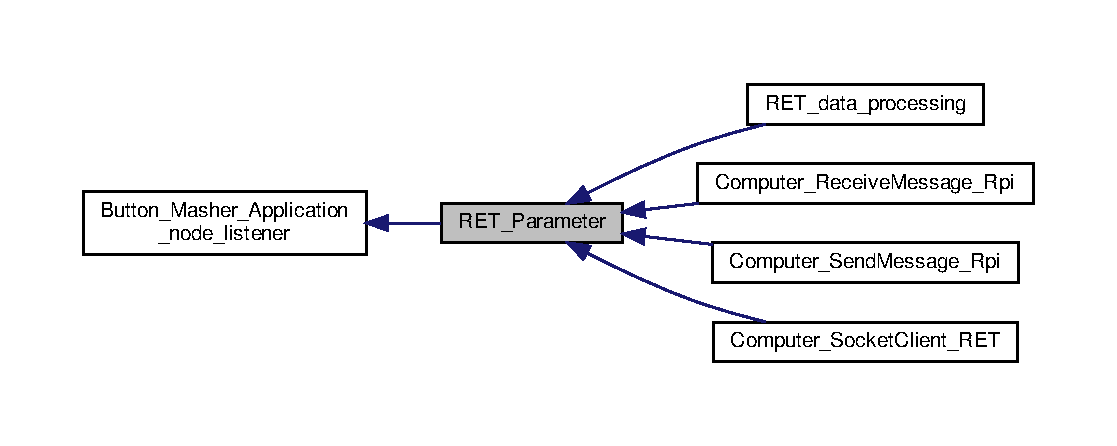
\includegraphics[width=350pt]{classRET__Parameter_1_1RET__Parameter__inherit__graph}
\end{center}
\end{figure}


Collaboration diagram for R\+E\+T\+\_\+\+Parameter\+:
\nopagebreak
\begin{figure}[H]
\begin{center}
\leavevmode
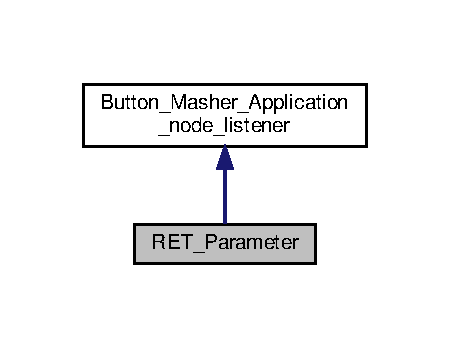
\includegraphics[width=216pt]{classRET__Parameter_1_1RET__Parameter__coll__graph}
\end{center}
\end{figure}
\subsection*{Public Member Functions}
\begin{DoxyCompactItemize}
\item 
def \hyperlink{classRET__Parameter_1_1RET__Parameter_acaff5a3a7b875ffce45f9c16a3f191d6}{\+\_\+\+\_\+init\+\_\+\+\_\+} (self, Button\+Masher\+Application\+\_\+output, \hyperlink{classRET__Parameter_1_1RET__Parameter_ac4848af5696d2d98e426d3d775d6964d}{list\+\_\+buttons\+\_\+area})
\begin{DoxyCompactList}\small\item\em The \hyperlink{classRET__Parameter_1_1RET__Parameter}{R\+E\+T\+\_\+\+Parameter} base class initializer. \end{DoxyCompactList}\item 
def \hyperlink{classRET__Parameter_1_1RET__Parameter_a6b5778a011cd40b8302107493f8212c3}{open\+\_\+csv\+\_\+file} (self)
\begin{DoxyCompactList}\small\item\em Retrieves the csv logfile we are logging the data in. \end{DoxyCompactList}\end{DoxyCompactItemize}
\subsection*{Public Attributes}
\begin{DoxyCompactItemize}
\item 
\hyperlink{classRET__Parameter_1_1RET__Parameter_abd224cfc80b136898df89af7812fa8d5}{acceleration\+\_\+factor}
\item 
\hyperlink{classRET__Parameter_1_1RET__Parameter_a39e93ce131ad25f98c5ce27c3ab36a6e}{Btn\+\_\+\+Pressed\+\_\+\+Time}
\item 
\hyperlink{classRET__Parameter_1_1RET__Parameter_a2b7700878675832931a1182c86c13de3}{Btn\+Masher\+Application\+\_\+output}
\begin{DoxyCompactList}\small\item\em Parameter about the Button Masher Application output. \end{DoxyCompactList}\item 
\hyperlink{classRET__Parameter_1_1RET__Parameter_a62209bbfef695c79e2e4a3c58cde6904}{button\+\_\+names}
\begin{DoxyCompactList}\small\item\em information about the measurement \end{DoxyCompactList}\item 
\hyperlink{classRET__Parameter_1_1RET__Parameter_a6a998519b5c6ea893e0afee65eccbf93}{csv\+\_\+header}
\item 
\hyperlink{classRET__Parameter_1_1RET__Parameter_a195beb1936a2c54c9c5b84ee44779c23}{csv\+\_\+name\+\_\+file}
\begin{DoxyCompactList}\small\item\em parameter for writing csv\+\_\+file \end{DoxyCompactList}\item 
\hyperlink{classRET__Parameter_1_1RET__Parameter_ac1a9a183848e43cc95622a427a79fffe}{end\+\_\+effector\+\_\+position\+\_\+entering\+\_\+button\+\_\+area}
\item 
\hyperlink{classRET__Parameter_1_1RET__Parameter_a9c8c6317198ca7fcf65796f882f5c428}{end\+\_\+effector\+\_\+position\+\_\+leaving\+\_\+button\+\_\+area}
\item 
\hyperlink{classRET__Parameter_1_1RET__Parameter_a1e5d03d6109af678189c173702b43d8a}{end\+\_\+effector\+\_\+position\+\_\+received\+\_\+socket\+\_\+message\+\_\+pressed}
\item 
\hyperlink{classRET__Parameter_1_1RET__Parameter_a034f595b48aad7217bd228d3620eaca8}{influxdb}
\item 
\hyperlink{classRET__Parameter_1_1RET__Parameter_a2c910a8a000ce837b18cf2959297dcce}{influxdb\+\_\+host}
\begin{DoxyCompactList}\small\item\em Parameter concerning the influxdb writing static parameter. \end{DoxyCompactList}\item 
\hyperlink{classRET__Parameter_1_1RET__Parameter_a2951333e048b79a878571eafd1eee541}{influxdb\+\_\+measurement}
\item 
\hyperlink{classRET__Parameter_1_1RET__Parameter_a0d892e15d9fa78818d4495560d962ec2}{influxdb\+\_\+port}
\item 
\hyperlink{classRET__Parameter_1_1RET__Parameter_a19e1c5b8812bb41ecaa59c174a9cc027}{list\+\_\+bouncetime}
\item 
\hyperlink{classRET__Parameter_1_1RET__Parameter_ac4848af5696d2d98e426d3d775d6964d}{list\+\_\+buttons\+\_\+area}
\item 
\hyperlink{classRET__Parameter_1_1RET__Parameter_ae07c53483c9c3ff8611ec4d7401fa71f}{list\+\_\+buttons\+\_\+positions}
\item 
\hyperlink{classRET__Parameter_1_1RET__Parameter_a356b7bcae5e020489b6db1128e16d11b}{list\+\_\+msg\+\_\+\+Btn\+\_\+\+Pressed}
\begin{DoxyCompactList}\small\item\em changing parameter \end{DoxyCompactList}\item 
\hyperlink{classRET__Parameter_1_1RET__Parameter_af4093e533290b780aa3d5611f6a8a526}{list\+\_\+to\+\_\+log}
\item 
\hyperlink{classRET__Parameter_1_1RET__Parameter_accada53c1f876f08e9c5beb661846ca1}{R\+E\+T\+\_\+driver}
\item 
\hyperlink{classRET__Parameter_1_1RET__Parameter_a153ea6721b57c14eea55728d46eae779}{robot\+\_\+settle\+\_\+time}
\item 
\hyperlink{classRET__Parameter_1_1RET__Parameter_afc570ca4c1952bb0a14a0511160df54a}{socket\+\_\+host}
\begin{DoxyCompactList}\small\item\em Parameter concerning the socket message static parameter. \end{DoxyCompactList}\item 
\hyperlink{classRET__Parameter_1_1RET__Parameter_a736f9eb916b0d398d68fc3e0c8f3f953}{socket\+\_\+port}
\item 
\hyperlink{classRET__Parameter_1_1RET__Parameter_a05a671c66aefea124cc08b76ea6d30bb}{test}
\item 
\hyperlink{classRET__Parameter_1_1RET__Parameter_a0fc681ced6250a0d860270ba7db63e5a}{time\+\_\+begin\+\_\+\+R\+ET}
\begin{DoxyCompactList}\small\item\em Global Parameter of the R\+ET. \end{DoxyCompactList}\item 
\hyperlink{classRET__Parameter_1_1RET__Parameter_aeb9535b7bbd9a71cd537b64de9a114f2}{time\+\_\+\+Btn\+\_\+\+Pressed}
\item 
\hyperlink{classRET__Parameter_1_1RET__Parameter_a1dbe7829bfc697ea985c80c74990e641}{time\+\_\+\+End\+\_\+\+Effector\+\_\+entering\+\_\+\+Btn\+\_\+\+Area}
\item 
\hyperlink{classRET__Parameter_1_1RET__Parameter_ab4ac422d38097f009ddb2c18a4172740}{time\+\_\+\+End\+\_\+\+Effector\+\_\+leaving\+\_\+\+Btn\+\_\+\+Area}
\item 
\hyperlink{classRET__Parameter_1_1RET__Parameter_ac753e4e4f67db35f3e3a49d6e329cd1a}{time\+\_\+inside\+\_\+button\+\_\+area}
\item 
\hyperlink{classRET__Parameter_1_1RET__Parameter_a082e6ba9804a6094336b4c267262460e}{velocity\+\_\+factor}
\item 
\hyperlink{classRET__Parameter_1_1RET__Parameter_a96204c1a4417d5a3a980521f8a66a1fa}{working\+\_\+on\+\_\+button}
\begin{DoxyCompactList}\small\item\em changing parameter \end{DoxyCompactList}\end{DoxyCompactItemize}


\subsection{Detailed Description}
The input of this function is the cartesian position of the end effector given by another node!!!!!!!!!!!!!!! 

The \hyperlink{classRET__Parameter_1_1RET__Parameter}{R\+E\+T\+\_\+\+Parameter} base class. Defines the base class utilized by all classes in the R\+ET. 

\subsection{Constructor \& Destructor Documentation}
\mbox{\Hypertarget{classRET__Parameter_1_1RET__Parameter_acaff5a3a7b875ffce45f9c16a3f191d6}\label{classRET__Parameter_1_1RET__Parameter_acaff5a3a7b875ffce45f9c16a3f191d6}} 
\index{R\+E\+T\+\_\+\+Parameter\+::\+R\+E\+T\+\_\+\+Parameter@{R\+E\+T\+\_\+\+Parameter\+::\+R\+E\+T\+\_\+\+Parameter}!\+\_\+\+\_\+init\+\_\+\+\_\+@{\+\_\+\+\_\+init\+\_\+\+\_\+}}
\index{\+\_\+\+\_\+init\+\_\+\+\_\+@{\+\_\+\+\_\+init\+\_\+\+\_\+}!R\+E\+T\+\_\+\+Parameter\+::\+R\+E\+T\+\_\+\+Parameter@{R\+E\+T\+\_\+\+Parameter\+::\+R\+E\+T\+\_\+\+Parameter}}
\subsubsection{\texorpdfstring{\+\_\+\+\_\+init\+\_\+\+\_\+()}{\_\_init\_\_()}}
{\footnotesize\ttfamily def \+\_\+\+\_\+init\+\_\+\+\_\+ (\begin{DoxyParamCaption}\item[{}]{self,  }\item[{}]{Button\+Masher\+Application\+\_\+output,  }\item[{}]{list\+\_\+buttons\+\_\+area }\end{DoxyParamCaption})}



The \hyperlink{classRET__Parameter_1_1RET__Parameter}{R\+E\+T\+\_\+\+Parameter} base class initializer. 


\begin{DoxyParams}{Parameters}
{\em Button\+Masher\+Application\+\_\+output} & The end effector cartesian position. \\
\hline
{\em list\+\_\+buttons\+\_\+area} & The list of the buttons\textquotesingle{}area we are working with. \\
\hline
\end{DoxyParams}
\begin{DoxyReturn}{Returns}
An instance of the R\+E\+T\+\_\+parameter class initialized with the specified name. 
\end{DoxyReturn}


\subsection{Member Function Documentation}
\mbox{\Hypertarget{classRET__Parameter_1_1RET__Parameter_a6b5778a011cd40b8302107493f8212c3}\label{classRET__Parameter_1_1RET__Parameter_a6b5778a011cd40b8302107493f8212c3}} 
\index{R\+E\+T\+\_\+\+Parameter\+::\+R\+E\+T\+\_\+\+Parameter@{R\+E\+T\+\_\+\+Parameter\+::\+R\+E\+T\+\_\+\+Parameter}!open\+\_\+csv\+\_\+file@{open\+\_\+csv\+\_\+file}}
\index{open\+\_\+csv\+\_\+file@{open\+\_\+csv\+\_\+file}!R\+E\+T\+\_\+\+Parameter\+::\+R\+E\+T\+\_\+\+Parameter@{R\+E\+T\+\_\+\+Parameter\+::\+R\+E\+T\+\_\+\+Parameter}}
\subsubsection{\texorpdfstring{open\+\_\+csv\+\_\+file()}{open\_csv\_file()}}
{\footnotesize\ttfamily def open\+\_\+csv\+\_\+file (\begin{DoxyParamCaption}\item[{}]{self }\end{DoxyParamCaption})}



Retrieves the csv logfile we are logging the data in. 

\begin{DoxyReturn}{Returns}
a csv file where we can log the data for a R\+ET. 
\end{DoxyReturn}


\subsection{Member Data Documentation}
\mbox{\Hypertarget{classRET__Parameter_1_1RET__Parameter_abd224cfc80b136898df89af7812fa8d5}\label{classRET__Parameter_1_1RET__Parameter_abd224cfc80b136898df89af7812fa8d5}} 
\index{R\+E\+T\+\_\+\+Parameter\+::\+R\+E\+T\+\_\+\+Parameter@{R\+E\+T\+\_\+\+Parameter\+::\+R\+E\+T\+\_\+\+Parameter}!acceleration\+\_\+factor@{acceleration\+\_\+factor}}
\index{acceleration\+\_\+factor@{acceleration\+\_\+factor}!R\+E\+T\+\_\+\+Parameter\+::\+R\+E\+T\+\_\+\+Parameter@{R\+E\+T\+\_\+\+Parameter\+::\+R\+E\+T\+\_\+\+Parameter}}
\subsubsection{\texorpdfstring{acceleration\+\_\+factor}{acceleration\_factor}}
{\footnotesize\ttfamily acceleration\+\_\+factor}

\mbox{\Hypertarget{classRET__Parameter_1_1RET__Parameter_a39e93ce131ad25f98c5ce27c3ab36a6e}\label{classRET__Parameter_1_1RET__Parameter_a39e93ce131ad25f98c5ce27c3ab36a6e}} 
\index{R\+E\+T\+\_\+\+Parameter\+::\+R\+E\+T\+\_\+\+Parameter@{R\+E\+T\+\_\+\+Parameter\+::\+R\+E\+T\+\_\+\+Parameter}!Btn\+\_\+\+Pressed\+\_\+\+Time@{Btn\+\_\+\+Pressed\+\_\+\+Time}}
\index{Btn\+\_\+\+Pressed\+\_\+\+Time@{Btn\+\_\+\+Pressed\+\_\+\+Time}!R\+E\+T\+\_\+\+Parameter\+::\+R\+E\+T\+\_\+\+Parameter@{R\+E\+T\+\_\+\+Parameter\+::\+R\+E\+T\+\_\+\+Parameter}}
\subsubsection{\texorpdfstring{Btn\+\_\+\+Pressed\+\_\+\+Time}{Btn\_Pressed\_Time}}
{\footnotesize\ttfamily Btn\+\_\+\+Pressed\+\_\+\+Time}

\mbox{\Hypertarget{classRET__Parameter_1_1RET__Parameter_a2b7700878675832931a1182c86c13de3}\label{classRET__Parameter_1_1RET__Parameter_a2b7700878675832931a1182c86c13de3}} 
\index{R\+E\+T\+\_\+\+Parameter\+::\+R\+E\+T\+\_\+\+Parameter@{R\+E\+T\+\_\+\+Parameter\+::\+R\+E\+T\+\_\+\+Parameter}!Btn\+Masher\+Application\+\_\+output@{Btn\+Masher\+Application\+\_\+output}}
\index{Btn\+Masher\+Application\+\_\+output@{Btn\+Masher\+Application\+\_\+output}!R\+E\+T\+\_\+\+Parameter\+::\+R\+E\+T\+\_\+\+Parameter@{R\+E\+T\+\_\+\+Parameter\+::\+R\+E\+T\+\_\+\+Parameter}}
\subsubsection{\texorpdfstring{Btn\+Masher\+Application\+\_\+output}{BtnMasherApplication\_output}}
{\footnotesize\ttfamily Btn\+Masher\+Application\+\_\+output}



Parameter about the Button Masher Application output. 

\mbox{\Hypertarget{classRET__Parameter_1_1RET__Parameter_a62209bbfef695c79e2e4a3c58cde6904}\label{classRET__Parameter_1_1RET__Parameter_a62209bbfef695c79e2e4a3c58cde6904}} 
\index{R\+E\+T\+\_\+\+Parameter\+::\+R\+E\+T\+\_\+\+Parameter@{R\+E\+T\+\_\+\+Parameter\+::\+R\+E\+T\+\_\+\+Parameter}!button\+\_\+names@{button\+\_\+names}}
\index{button\+\_\+names@{button\+\_\+names}!R\+E\+T\+\_\+\+Parameter\+::\+R\+E\+T\+\_\+\+Parameter@{R\+E\+T\+\_\+\+Parameter\+::\+R\+E\+T\+\_\+\+Parameter}}
\subsubsection{\texorpdfstring{button\+\_\+names}{button\_names}}
{\footnotesize\ttfamily button\+\_\+names}



information about the measurement 

\mbox{\Hypertarget{classRET__Parameter_1_1RET__Parameter_a6a998519b5c6ea893e0afee65eccbf93}\label{classRET__Parameter_1_1RET__Parameter_a6a998519b5c6ea893e0afee65eccbf93}} 
\index{R\+E\+T\+\_\+\+Parameter\+::\+R\+E\+T\+\_\+\+Parameter@{R\+E\+T\+\_\+\+Parameter\+::\+R\+E\+T\+\_\+\+Parameter}!csv\+\_\+header@{csv\+\_\+header}}
\index{csv\+\_\+header@{csv\+\_\+header}!R\+E\+T\+\_\+\+Parameter\+::\+R\+E\+T\+\_\+\+Parameter@{R\+E\+T\+\_\+\+Parameter\+::\+R\+E\+T\+\_\+\+Parameter}}
\subsubsection{\texorpdfstring{csv\+\_\+header}{csv\_header}}
{\footnotesize\ttfamily csv\+\_\+header}

\mbox{\Hypertarget{classRET__Parameter_1_1RET__Parameter_a195beb1936a2c54c9c5b84ee44779c23}\label{classRET__Parameter_1_1RET__Parameter_a195beb1936a2c54c9c5b84ee44779c23}} 
\index{R\+E\+T\+\_\+\+Parameter\+::\+R\+E\+T\+\_\+\+Parameter@{R\+E\+T\+\_\+\+Parameter\+::\+R\+E\+T\+\_\+\+Parameter}!csv\+\_\+name\+\_\+file@{csv\+\_\+name\+\_\+file}}
\index{csv\+\_\+name\+\_\+file@{csv\+\_\+name\+\_\+file}!R\+E\+T\+\_\+\+Parameter\+::\+R\+E\+T\+\_\+\+Parameter@{R\+E\+T\+\_\+\+Parameter\+::\+R\+E\+T\+\_\+\+Parameter}}
\subsubsection{\texorpdfstring{csv\+\_\+name\+\_\+file}{csv\_name\_file}}
{\footnotesize\ttfamily csv\+\_\+name\+\_\+file}



parameter for writing csv\+\_\+file 

\mbox{\Hypertarget{classRET__Parameter_1_1RET__Parameter_ac1a9a183848e43cc95622a427a79fffe}\label{classRET__Parameter_1_1RET__Parameter_ac1a9a183848e43cc95622a427a79fffe}} 
\index{R\+E\+T\+\_\+\+Parameter\+::\+R\+E\+T\+\_\+\+Parameter@{R\+E\+T\+\_\+\+Parameter\+::\+R\+E\+T\+\_\+\+Parameter}!end\+\_\+effector\+\_\+position\+\_\+entering\+\_\+button\+\_\+area@{end\+\_\+effector\+\_\+position\+\_\+entering\+\_\+button\+\_\+area}}
\index{end\+\_\+effector\+\_\+position\+\_\+entering\+\_\+button\+\_\+area@{end\+\_\+effector\+\_\+position\+\_\+entering\+\_\+button\+\_\+area}!R\+E\+T\+\_\+\+Parameter\+::\+R\+E\+T\+\_\+\+Parameter@{R\+E\+T\+\_\+\+Parameter\+::\+R\+E\+T\+\_\+\+Parameter}}
\subsubsection{\texorpdfstring{end\+\_\+effector\+\_\+position\+\_\+entering\+\_\+button\+\_\+area}{end\_effector\_position\_entering\_button\_area}}
{\footnotesize\ttfamily end\+\_\+effector\+\_\+position\+\_\+entering\+\_\+button\+\_\+area}

\mbox{\Hypertarget{classRET__Parameter_1_1RET__Parameter_a9c8c6317198ca7fcf65796f882f5c428}\label{classRET__Parameter_1_1RET__Parameter_a9c8c6317198ca7fcf65796f882f5c428}} 
\index{R\+E\+T\+\_\+\+Parameter\+::\+R\+E\+T\+\_\+\+Parameter@{R\+E\+T\+\_\+\+Parameter\+::\+R\+E\+T\+\_\+\+Parameter}!end\+\_\+effector\+\_\+position\+\_\+leaving\+\_\+button\+\_\+area@{end\+\_\+effector\+\_\+position\+\_\+leaving\+\_\+button\+\_\+area}}
\index{end\+\_\+effector\+\_\+position\+\_\+leaving\+\_\+button\+\_\+area@{end\+\_\+effector\+\_\+position\+\_\+leaving\+\_\+button\+\_\+area}!R\+E\+T\+\_\+\+Parameter\+::\+R\+E\+T\+\_\+\+Parameter@{R\+E\+T\+\_\+\+Parameter\+::\+R\+E\+T\+\_\+\+Parameter}}
\subsubsection{\texorpdfstring{end\+\_\+effector\+\_\+position\+\_\+leaving\+\_\+button\+\_\+area}{end\_effector\_position\_leaving\_button\_area}}
{\footnotesize\ttfamily end\+\_\+effector\+\_\+position\+\_\+leaving\+\_\+button\+\_\+area}

\mbox{\Hypertarget{classRET__Parameter_1_1RET__Parameter_a1e5d03d6109af678189c173702b43d8a}\label{classRET__Parameter_1_1RET__Parameter_a1e5d03d6109af678189c173702b43d8a}} 
\index{R\+E\+T\+\_\+\+Parameter\+::\+R\+E\+T\+\_\+\+Parameter@{R\+E\+T\+\_\+\+Parameter\+::\+R\+E\+T\+\_\+\+Parameter}!end\+\_\+effector\+\_\+position\+\_\+received\+\_\+socket\+\_\+message\+\_\+pressed@{end\+\_\+effector\+\_\+position\+\_\+received\+\_\+socket\+\_\+message\+\_\+pressed}}
\index{end\+\_\+effector\+\_\+position\+\_\+received\+\_\+socket\+\_\+message\+\_\+pressed@{end\+\_\+effector\+\_\+position\+\_\+received\+\_\+socket\+\_\+message\+\_\+pressed}!R\+E\+T\+\_\+\+Parameter\+::\+R\+E\+T\+\_\+\+Parameter@{R\+E\+T\+\_\+\+Parameter\+::\+R\+E\+T\+\_\+\+Parameter}}
\subsubsection{\texorpdfstring{end\+\_\+effector\+\_\+position\+\_\+received\+\_\+socket\+\_\+message\+\_\+pressed}{end\_effector\_position\_received\_socket\_message\_pressed}}
{\footnotesize\ttfamily end\+\_\+effector\+\_\+position\+\_\+received\+\_\+socket\+\_\+message\+\_\+pressed}

\mbox{\Hypertarget{classRET__Parameter_1_1RET__Parameter_a034f595b48aad7217bd228d3620eaca8}\label{classRET__Parameter_1_1RET__Parameter_a034f595b48aad7217bd228d3620eaca8}} 
\index{R\+E\+T\+\_\+\+Parameter\+::\+R\+E\+T\+\_\+\+Parameter@{R\+E\+T\+\_\+\+Parameter\+::\+R\+E\+T\+\_\+\+Parameter}!influxdb@{influxdb}}
\index{influxdb@{influxdb}!R\+E\+T\+\_\+\+Parameter\+::\+R\+E\+T\+\_\+\+Parameter@{R\+E\+T\+\_\+\+Parameter\+::\+R\+E\+T\+\_\+\+Parameter}}
\subsubsection{\texorpdfstring{influxdb}{influxdb}}
{\footnotesize\ttfamily influxdb}

\mbox{\Hypertarget{classRET__Parameter_1_1RET__Parameter_a2c910a8a000ce837b18cf2959297dcce}\label{classRET__Parameter_1_1RET__Parameter_a2c910a8a000ce837b18cf2959297dcce}} 
\index{R\+E\+T\+\_\+\+Parameter\+::\+R\+E\+T\+\_\+\+Parameter@{R\+E\+T\+\_\+\+Parameter\+::\+R\+E\+T\+\_\+\+Parameter}!influxdb\+\_\+host@{influxdb\+\_\+host}}
\index{influxdb\+\_\+host@{influxdb\+\_\+host}!R\+E\+T\+\_\+\+Parameter\+::\+R\+E\+T\+\_\+\+Parameter@{R\+E\+T\+\_\+\+Parameter\+::\+R\+E\+T\+\_\+\+Parameter}}
\subsubsection{\texorpdfstring{influxdb\+\_\+host}{influxdb\_host}}
{\footnotesize\ttfamily influxdb\+\_\+host}



Parameter concerning the influxdb writing static parameter. 

\mbox{\Hypertarget{classRET__Parameter_1_1RET__Parameter_a2951333e048b79a878571eafd1eee541}\label{classRET__Parameter_1_1RET__Parameter_a2951333e048b79a878571eafd1eee541}} 
\index{R\+E\+T\+\_\+\+Parameter\+::\+R\+E\+T\+\_\+\+Parameter@{R\+E\+T\+\_\+\+Parameter\+::\+R\+E\+T\+\_\+\+Parameter}!influxdb\+\_\+measurement@{influxdb\+\_\+measurement}}
\index{influxdb\+\_\+measurement@{influxdb\+\_\+measurement}!R\+E\+T\+\_\+\+Parameter\+::\+R\+E\+T\+\_\+\+Parameter@{R\+E\+T\+\_\+\+Parameter\+::\+R\+E\+T\+\_\+\+Parameter}}
\subsubsection{\texorpdfstring{influxdb\+\_\+measurement}{influxdb\_measurement}}
{\footnotesize\ttfamily influxdb\+\_\+measurement}

\mbox{\Hypertarget{classRET__Parameter_1_1RET__Parameter_a0d892e15d9fa78818d4495560d962ec2}\label{classRET__Parameter_1_1RET__Parameter_a0d892e15d9fa78818d4495560d962ec2}} 
\index{R\+E\+T\+\_\+\+Parameter\+::\+R\+E\+T\+\_\+\+Parameter@{R\+E\+T\+\_\+\+Parameter\+::\+R\+E\+T\+\_\+\+Parameter}!influxdb\+\_\+port@{influxdb\+\_\+port}}
\index{influxdb\+\_\+port@{influxdb\+\_\+port}!R\+E\+T\+\_\+\+Parameter\+::\+R\+E\+T\+\_\+\+Parameter@{R\+E\+T\+\_\+\+Parameter\+::\+R\+E\+T\+\_\+\+Parameter}}
\subsubsection{\texorpdfstring{influxdb\+\_\+port}{influxdb\_port}}
{\footnotesize\ttfamily influxdb\+\_\+port}

\mbox{\Hypertarget{classRET__Parameter_1_1RET__Parameter_a19e1c5b8812bb41ecaa59c174a9cc027}\label{classRET__Parameter_1_1RET__Parameter_a19e1c5b8812bb41ecaa59c174a9cc027}} 
\index{R\+E\+T\+\_\+\+Parameter\+::\+R\+E\+T\+\_\+\+Parameter@{R\+E\+T\+\_\+\+Parameter\+::\+R\+E\+T\+\_\+\+Parameter}!list\+\_\+bouncetime@{list\+\_\+bouncetime}}
\index{list\+\_\+bouncetime@{list\+\_\+bouncetime}!R\+E\+T\+\_\+\+Parameter\+::\+R\+E\+T\+\_\+\+Parameter@{R\+E\+T\+\_\+\+Parameter\+::\+R\+E\+T\+\_\+\+Parameter}}
\subsubsection{\texorpdfstring{list\+\_\+bouncetime}{list\_bouncetime}}
{\footnotesize\ttfamily list\+\_\+bouncetime}

\mbox{\Hypertarget{classRET__Parameter_1_1RET__Parameter_ac4848af5696d2d98e426d3d775d6964d}\label{classRET__Parameter_1_1RET__Parameter_ac4848af5696d2d98e426d3d775d6964d}} 
\index{R\+E\+T\+\_\+\+Parameter\+::\+R\+E\+T\+\_\+\+Parameter@{R\+E\+T\+\_\+\+Parameter\+::\+R\+E\+T\+\_\+\+Parameter}!list\+\_\+buttons\+\_\+area@{list\+\_\+buttons\+\_\+area}}
\index{list\+\_\+buttons\+\_\+area@{list\+\_\+buttons\+\_\+area}!R\+E\+T\+\_\+\+Parameter\+::\+R\+E\+T\+\_\+\+Parameter@{R\+E\+T\+\_\+\+Parameter\+::\+R\+E\+T\+\_\+\+Parameter}}
\subsubsection{\texorpdfstring{list\+\_\+buttons\+\_\+area}{list\_buttons\_area}}
{\footnotesize\ttfamily list\+\_\+buttons\+\_\+area}

\mbox{\Hypertarget{classRET__Parameter_1_1RET__Parameter_ae07c53483c9c3ff8611ec4d7401fa71f}\label{classRET__Parameter_1_1RET__Parameter_ae07c53483c9c3ff8611ec4d7401fa71f}} 
\index{R\+E\+T\+\_\+\+Parameter\+::\+R\+E\+T\+\_\+\+Parameter@{R\+E\+T\+\_\+\+Parameter\+::\+R\+E\+T\+\_\+\+Parameter}!list\+\_\+buttons\+\_\+positions@{list\+\_\+buttons\+\_\+positions}}
\index{list\+\_\+buttons\+\_\+positions@{list\+\_\+buttons\+\_\+positions}!R\+E\+T\+\_\+\+Parameter\+::\+R\+E\+T\+\_\+\+Parameter@{R\+E\+T\+\_\+\+Parameter\+::\+R\+E\+T\+\_\+\+Parameter}}
\subsubsection{\texorpdfstring{list\+\_\+buttons\+\_\+positions}{list\_buttons\_positions}}
{\footnotesize\ttfamily list\+\_\+buttons\+\_\+positions}

\mbox{\Hypertarget{classRET__Parameter_1_1RET__Parameter_a356b7bcae5e020489b6db1128e16d11b}\label{classRET__Parameter_1_1RET__Parameter_a356b7bcae5e020489b6db1128e16d11b}} 
\index{R\+E\+T\+\_\+\+Parameter\+::\+R\+E\+T\+\_\+\+Parameter@{R\+E\+T\+\_\+\+Parameter\+::\+R\+E\+T\+\_\+\+Parameter}!list\+\_\+msg\+\_\+\+Btn\+\_\+\+Pressed@{list\+\_\+msg\+\_\+\+Btn\+\_\+\+Pressed}}
\index{list\+\_\+msg\+\_\+\+Btn\+\_\+\+Pressed@{list\+\_\+msg\+\_\+\+Btn\+\_\+\+Pressed}!R\+E\+T\+\_\+\+Parameter\+::\+R\+E\+T\+\_\+\+Parameter@{R\+E\+T\+\_\+\+Parameter\+::\+R\+E\+T\+\_\+\+Parameter}}
\subsubsection{\texorpdfstring{list\+\_\+msg\+\_\+\+Btn\+\_\+\+Pressed}{list\_msg\_Btn\_Pressed}}
{\footnotesize\ttfamily list\+\_\+msg\+\_\+\+Btn\+\_\+\+Pressed}



changing parameter 

\mbox{\Hypertarget{classRET__Parameter_1_1RET__Parameter_af4093e533290b780aa3d5611f6a8a526}\label{classRET__Parameter_1_1RET__Parameter_af4093e533290b780aa3d5611f6a8a526}} 
\index{R\+E\+T\+\_\+\+Parameter\+::\+R\+E\+T\+\_\+\+Parameter@{R\+E\+T\+\_\+\+Parameter\+::\+R\+E\+T\+\_\+\+Parameter}!list\+\_\+to\+\_\+log@{list\+\_\+to\+\_\+log}}
\index{list\+\_\+to\+\_\+log@{list\+\_\+to\+\_\+log}!R\+E\+T\+\_\+\+Parameter\+::\+R\+E\+T\+\_\+\+Parameter@{R\+E\+T\+\_\+\+Parameter\+::\+R\+E\+T\+\_\+\+Parameter}}
\subsubsection{\texorpdfstring{list\+\_\+to\+\_\+log}{list\_to\_log}}
{\footnotesize\ttfamily list\+\_\+to\+\_\+log}

\mbox{\Hypertarget{classRET__Parameter_1_1RET__Parameter_accada53c1f876f08e9c5beb661846ca1}\label{classRET__Parameter_1_1RET__Parameter_accada53c1f876f08e9c5beb661846ca1}} 
\index{R\+E\+T\+\_\+\+Parameter\+::\+R\+E\+T\+\_\+\+Parameter@{R\+E\+T\+\_\+\+Parameter\+::\+R\+E\+T\+\_\+\+Parameter}!R\+E\+T\+\_\+driver@{R\+E\+T\+\_\+driver}}
\index{R\+E\+T\+\_\+driver@{R\+E\+T\+\_\+driver}!R\+E\+T\+\_\+\+Parameter\+::\+R\+E\+T\+\_\+\+Parameter@{R\+E\+T\+\_\+\+Parameter\+::\+R\+E\+T\+\_\+\+Parameter}}
\subsubsection{\texorpdfstring{R\+E\+T\+\_\+driver}{RET\_driver}}
{\footnotesize\ttfamily R\+E\+T\+\_\+driver}

\mbox{\Hypertarget{classRET__Parameter_1_1RET__Parameter_a153ea6721b57c14eea55728d46eae779}\label{classRET__Parameter_1_1RET__Parameter_a153ea6721b57c14eea55728d46eae779}} 
\index{R\+E\+T\+\_\+\+Parameter\+::\+R\+E\+T\+\_\+\+Parameter@{R\+E\+T\+\_\+\+Parameter\+::\+R\+E\+T\+\_\+\+Parameter}!robot\+\_\+settle\+\_\+time@{robot\+\_\+settle\+\_\+time}}
\index{robot\+\_\+settle\+\_\+time@{robot\+\_\+settle\+\_\+time}!R\+E\+T\+\_\+\+Parameter\+::\+R\+E\+T\+\_\+\+Parameter@{R\+E\+T\+\_\+\+Parameter\+::\+R\+E\+T\+\_\+\+Parameter}}
\subsubsection{\texorpdfstring{robot\+\_\+settle\+\_\+time}{robot\_settle\_time}}
{\footnotesize\ttfamily robot\+\_\+settle\+\_\+time}

\mbox{\Hypertarget{classRET__Parameter_1_1RET__Parameter_afc570ca4c1952bb0a14a0511160df54a}\label{classRET__Parameter_1_1RET__Parameter_afc570ca4c1952bb0a14a0511160df54a}} 
\index{R\+E\+T\+\_\+\+Parameter\+::\+R\+E\+T\+\_\+\+Parameter@{R\+E\+T\+\_\+\+Parameter\+::\+R\+E\+T\+\_\+\+Parameter}!socket\+\_\+host@{socket\+\_\+host}}
\index{socket\+\_\+host@{socket\+\_\+host}!R\+E\+T\+\_\+\+Parameter\+::\+R\+E\+T\+\_\+\+Parameter@{R\+E\+T\+\_\+\+Parameter\+::\+R\+E\+T\+\_\+\+Parameter}}
\subsubsection{\texorpdfstring{socket\+\_\+host}{socket\_host}}
{\footnotesize\ttfamily socket\+\_\+host}



Parameter concerning the socket message static parameter. 

\mbox{\Hypertarget{classRET__Parameter_1_1RET__Parameter_a736f9eb916b0d398d68fc3e0c8f3f953}\label{classRET__Parameter_1_1RET__Parameter_a736f9eb916b0d398d68fc3e0c8f3f953}} 
\index{R\+E\+T\+\_\+\+Parameter\+::\+R\+E\+T\+\_\+\+Parameter@{R\+E\+T\+\_\+\+Parameter\+::\+R\+E\+T\+\_\+\+Parameter}!socket\+\_\+port@{socket\+\_\+port}}
\index{socket\+\_\+port@{socket\+\_\+port}!R\+E\+T\+\_\+\+Parameter\+::\+R\+E\+T\+\_\+\+Parameter@{R\+E\+T\+\_\+\+Parameter\+::\+R\+E\+T\+\_\+\+Parameter}}
\subsubsection{\texorpdfstring{socket\+\_\+port}{socket\_port}}
{\footnotesize\ttfamily socket\+\_\+port}

\mbox{\Hypertarget{classRET__Parameter_1_1RET__Parameter_a05a671c66aefea124cc08b76ea6d30bb}\label{classRET__Parameter_1_1RET__Parameter_a05a671c66aefea124cc08b76ea6d30bb}} 
\index{R\+E\+T\+\_\+\+Parameter\+::\+R\+E\+T\+\_\+\+Parameter@{R\+E\+T\+\_\+\+Parameter\+::\+R\+E\+T\+\_\+\+Parameter}!test@{test}}
\index{test@{test}!R\+E\+T\+\_\+\+Parameter\+::\+R\+E\+T\+\_\+\+Parameter@{R\+E\+T\+\_\+\+Parameter\+::\+R\+E\+T\+\_\+\+Parameter}}
\subsubsection{\texorpdfstring{test}{test}}
{\footnotesize\ttfamily test}

\mbox{\Hypertarget{classRET__Parameter_1_1RET__Parameter_a0fc681ced6250a0d860270ba7db63e5a}\label{classRET__Parameter_1_1RET__Parameter_a0fc681ced6250a0d860270ba7db63e5a}} 
\index{R\+E\+T\+\_\+\+Parameter\+::\+R\+E\+T\+\_\+\+Parameter@{R\+E\+T\+\_\+\+Parameter\+::\+R\+E\+T\+\_\+\+Parameter}!time\+\_\+begin\+\_\+\+R\+ET@{time\+\_\+begin\+\_\+\+R\+ET}}
\index{time\+\_\+begin\+\_\+\+R\+ET@{time\+\_\+begin\+\_\+\+R\+ET}!R\+E\+T\+\_\+\+Parameter\+::\+R\+E\+T\+\_\+\+Parameter@{R\+E\+T\+\_\+\+Parameter\+::\+R\+E\+T\+\_\+\+Parameter}}
\subsubsection{\texorpdfstring{time\+\_\+begin\+\_\+\+R\+ET}{time\_begin\_RET}}
{\footnotesize\ttfamily time\+\_\+begin\+\_\+\+R\+ET}



Global Parameter of the R\+ET. 

\mbox{\Hypertarget{classRET__Parameter_1_1RET__Parameter_aeb9535b7bbd9a71cd537b64de9a114f2}\label{classRET__Parameter_1_1RET__Parameter_aeb9535b7bbd9a71cd537b64de9a114f2}} 
\index{R\+E\+T\+\_\+\+Parameter\+::\+R\+E\+T\+\_\+\+Parameter@{R\+E\+T\+\_\+\+Parameter\+::\+R\+E\+T\+\_\+\+Parameter}!time\+\_\+\+Btn\+\_\+\+Pressed@{time\+\_\+\+Btn\+\_\+\+Pressed}}
\index{time\+\_\+\+Btn\+\_\+\+Pressed@{time\+\_\+\+Btn\+\_\+\+Pressed}!R\+E\+T\+\_\+\+Parameter\+::\+R\+E\+T\+\_\+\+Parameter@{R\+E\+T\+\_\+\+Parameter\+::\+R\+E\+T\+\_\+\+Parameter}}
\subsubsection{\texorpdfstring{time\+\_\+\+Btn\+\_\+\+Pressed}{time\_Btn\_Pressed}}
{\footnotesize\ttfamily time\+\_\+\+Btn\+\_\+\+Pressed}

\mbox{\Hypertarget{classRET__Parameter_1_1RET__Parameter_a1dbe7829bfc697ea985c80c74990e641}\label{classRET__Parameter_1_1RET__Parameter_a1dbe7829bfc697ea985c80c74990e641}} 
\index{R\+E\+T\+\_\+\+Parameter\+::\+R\+E\+T\+\_\+\+Parameter@{R\+E\+T\+\_\+\+Parameter\+::\+R\+E\+T\+\_\+\+Parameter}!time\+\_\+\+End\+\_\+\+Effector\+\_\+entering\+\_\+\+Btn\+\_\+\+Area@{time\+\_\+\+End\+\_\+\+Effector\+\_\+entering\+\_\+\+Btn\+\_\+\+Area}}
\index{time\+\_\+\+End\+\_\+\+Effector\+\_\+entering\+\_\+\+Btn\+\_\+\+Area@{time\+\_\+\+End\+\_\+\+Effector\+\_\+entering\+\_\+\+Btn\+\_\+\+Area}!R\+E\+T\+\_\+\+Parameter\+::\+R\+E\+T\+\_\+\+Parameter@{R\+E\+T\+\_\+\+Parameter\+::\+R\+E\+T\+\_\+\+Parameter}}
\subsubsection{\texorpdfstring{time\+\_\+\+End\+\_\+\+Effector\+\_\+entering\+\_\+\+Btn\+\_\+\+Area}{time\_End\_Effector\_entering\_Btn\_Area}}
{\footnotesize\ttfamily time\+\_\+\+End\+\_\+\+Effector\+\_\+entering\+\_\+\+Btn\+\_\+\+Area}

\mbox{\Hypertarget{classRET__Parameter_1_1RET__Parameter_ab4ac422d38097f009ddb2c18a4172740}\label{classRET__Parameter_1_1RET__Parameter_ab4ac422d38097f009ddb2c18a4172740}} 
\index{R\+E\+T\+\_\+\+Parameter\+::\+R\+E\+T\+\_\+\+Parameter@{R\+E\+T\+\_\+\+Parameter\+::\+R\+E\+T\+\_\+\+Parameter}!time\+\_\+\+End\+\_\+\+Effector\+\_\+leaving\+\_\+\+Btn\+\_\+\+Area@{time\+\_\+\+End\+\_\+\+Effector\+\_\+leaving\+\_\+\+Btn\+\_\+\+Area}}
\index{time\+\_\+\+End\+\_\+\+Effector\+\_\+leaving\+\_\+\+Btn\+\_\+\+Area@{time\+\_\+\+End\+\_\+\+Effector\+\_\+leaving\+\_\+\+Btn\+\_\+\+Area}!R\+E\+T\+\_\+\+Parameter\+::\+R\+E\+T\+\_\+\+Parameter@{R\+E\+T\+\_\+\+Parameter\+::\+R\+E\+T\+\_\+\+Parameter}}
\subsubsection{\texorpdfstring{time\+\_\+\+End\+\_\+\+Effector\+\_\+leaving\+\_\+\+Btn\+\_\+\+Area}{time\_End\_Effector\_leaving\_Btn\_Area}}
{\footnotesize\ttfamily time\+\_\+\+End\+\_\+\+Effector\+\_\+leaving\+\_\+\+Btn\+\_\+\+Area}

\mbox{\Hypertarget{classRET__Parameter_1_1RET__Parameter_ac753e4e4f67db35f3e3a49d6e329cd1a}\label{classRET__Parameter_1_1RET__Parameter_ac753e4e4f67db35f3e3a49d6e329cd1a}} 
\index{R\+E\+T\+\_\+\+Parameter\+::\+R\+E\+T\+\_\+\+Parameter@{R\+E\+T\+\_\+\+Parameter\+::\+R\+E\+T\+\_\+\+Parameter}!time\+\_\+inside\+\_\+button\+\_\+area@{time\+\_\+inside\+\_\+button\+\_\+area}}
\index{time\+\_\+inside\+\_\+button\+\_\+area@{time\+\_\+inside\+\_\+button\+\_\+area}!R\+E\+T\+\_\+\+Parameter\+::\+R\+E\+T\+\_\+\+Parameter@{R\+E\+T\+\_\+\+Parameter\+::\+R\+E\+T\+\_\+\+Parameter}}
\subsubsection{\texorpdfstring{time\+\_\+inside\+\_\+button\+\_\+area}{time\_inside\_button\_area}}
{\footnotesize\ttfamily time\+\_\+inside\+\_\+button\+\_\+area}

\mbox{\Hypertarget{classRET__Parameter_1_1RET__Parameter_a082e6ba9804a6094336b4c267262460e}\label{classRET__Parameter_1_1RET__Parameter_a082e6ba9804a6094336b4c267262460e}} 
\index{R\+E\+T\+\_\+\+Parameter\+::\+R\+E\+T\+\_\+\+Parameter@{R\+E\+T\+\_\+\+Parameter\+::\+R\+E\+T\+\_\+\+Parameter}!velocity\+\_\+factor@{velocity\+\_\+factor}}
\index{velocity\+\_\+factor@{velocity\+\_\+factor}!R\+E\+T\+\_\+\+Parameter\+::\+R\+E\+T\+\_\+\+Parameter@{R\+E\+T\+\_\+\+Parameter\+::\+R\+E\+T\+\_\+\+Parameter}}
\subsubsection{\texorpdfstring{velocity\+\_\+factor}{velocity\_factor}}
{\footnotesize\ttfamily velocity\+\_\+factor}

\mbox{\Hypertarget{classRET__Parameter_1_1RET__Parameter_a96204c1a4417d5a3a980521f8a66a1fa}\label{classRET__Parameter_1_1RET__Parameter_a96204c1a4417d5a3a980521f8a66a1fa}} 
\index{R\+E\+T\+\_\+\+Parameter\+::\+R\+E\+T\+\_\+\+Parameter@{R\+E\+T\+\_\+\+Parameter\+::\+R\+E\+T\+\_\+\+Parameter}!working\+\_\+on\+\_\+button@{working\+\_\+on\+\_\+button}}
\index{working\+\_\+on\+\_\+button@{working\+\_\+on\+\_\+button}!R\+E\+T\+\_\+\+Parameter\+::\+R\+E\+T\+\_\+\+Parameter@{R\+E\+T\+\_\+\+Parameter\+::\+R\+E\+T\+\_\+\+Parameter}}
\subsubsection{\texorpdfstring{working\+\_\+on\+\_\+button}{working\_on\_button}}
{\footnotesize\ttfamily working\+\_\+on\+\_\+button}



changing parameter 



The documentation for this class was generated from the following file\+:\begin{DoxyCompactItemize}
\item 
/home/ret/workspaces/ret/src/ret/scripts/\hyperlink{RET__Parameter_8py}{R\+E\+T\+\_\+\+Parameter.\+py}\end{DoxyCompactItemize}

\chapter{File Documentation}
\hypertarget{Button__Masher__Application__Output_8py}{}\section{/home/ret/workspaces/ret/src/ret/scripts/\+Button\+\_\+\+Masher\+\_\+\+Application\+\_\+\+Output.py File Reference}
\label{Button__Masher__Application__Output_8py}\index{/home/ret/workspaces/ret/src/ret/scripts/\+Button\+\_\+\+Masher\+\_\+\+Application\+\_\+\+Output.\+py@{/home/ret/workspaces/ret/src/ret/scripts/\+Button\+\_\+\+Masher\+\_\+\+Application\+\_\+\+Output.\+py}}
\subsection*{Classes}
\begin{DoxyCompactItemize}
\item 
class \hyperlink{classButton__Masher__Application__Output_1_1Button__Masher__Application__node__listener}{Button\+\_\+\+Masher\+\_\+\+Application\+\_\+node\+\_\+listener}
\begin{DoxyCompactList}\small\item\em The \hyperlink{classButton__Masher__Application__Output_1_1Button__Masher__Application__node__listener}{Button\+\_\+\+Masher\+\_\+\+Application\+\_\+node\+\_\+listener} base class. \end{DoxyCompactList}\end{DoxyCompactItemize}
\subsection*{Namespaces}
\begin{DoxyCompactItemize}
\item 
 \hyperlink{namespaceButton__Masher__Application__Output}{Button\+\_\+\+Masher\+\_\+\+Application\+\_\+\+Output}
\end{DoxyCompactItemize}
\subsection*{Functions}
\begin{DoxyCompactItemize}
\item 
def \hyperlink{namespaceButton__Masher__Application__Output_ad537c35a13781c3e28b4e3cc57ba321e}{launch\+\_\+node\+\_\+listener} ()
\begin{DoxyCompactList}\small\item\em Initialize the node tool\+\_\+pose\+\_\+publisher\+\_\+use. \end{DoxyCompactList}\end{DoxyCompactItemize}

\hypertarget{RET__config_8py}{}\section{/home/ret/workspaces/ret/src/ret/scripts/\+R\+E\+T\+\_\+config.py File Reference}
\label{RET__config_8py}\index{/home/ret/workspaces/ret/src/ret/scripts/\+R\+E\+T\+\_\+config.\+py@{/home/ret/workspaces/ret/src/ret/scripts/\+R\+E\+T\+\_\+config.\+py}}
\subsection*{Classes}
\begin{DoxyCompactItemize}
\item 
class \hyperlink{classRET__config_1_1Btn}{Btn}
\begin{DoxyCompactList}\small\item\em The \hyperlink{classRET__config_1_1Btn}{Btn} base class. \end{DoxyCompactList}\item 
class \hyperlink{classRET__config_1_1Btn__area}{Btn\+\_\+area}
\begin{DoxyCompactList}\small\item\em The \hyperlink{classRET__config_1_1Btn__area}{Btn\+\_\+area} class. \end{DoxyCompactList}\end{DoxyCompactItemize}
\subsection*{Namespaces}
\begin{DoxyCompactItemize}
\item 
 \hyperlink{namespaceRET__config}{R\+E\+T\+\_\+config}
\end{DoxyCompactItemize}
\subsection*{Variables}
\begin{DoxyCompactItemize}
\item 
float \hyperlink{namespaceRET__config_a425bc201cf7b10f0c4f1068f752e7c9b}{acceleration\+\_\+factor} = 3.\+49
\item 
\hyperlink{namespaceRET__config_af037c6b9ff0314103d8127acc9d07e0b}{Btn1} = Btn(\char`\"{}Btn1\char`\"{},x1,y1,z1)
\item 
\hyperlink{namespaceRET__config_a118140d2896d1aff1e3c9355f9deb314}{Btn1\+\_\+area} = Btn\+\_\+area(Btn1, delta\+\_\+area\mbox{[}0\mbox{]}, delta\+\_\+area\mbox{[}1\mbox{]}, delta\+\_\+area\mbox{[}2\mbox{]})
\item 
\hyperlink{namespaceRET__config_a73afa8c52cebd94e1889df5fbe3bec66}{Btn2} = Btn(\char`\"{}Btn2\char`\"{},x2,y2,z2)
\item 
\hyperlink{namespaceRET__config_a51a4083768cbc17b22a98ad63a7bf851}{Btn2\+\_\+area} = Btn\+\_\+area(Btn2, delta\+\_\+area\mbox{[}0\mbox{]}, delta\+\_\+area\mbox{[}1\mbox{]}, delta\+\_\+area\mbox{[}2\mbox{]})
\item 
list \hyperlink{namespaceRET__config_abbf3fd8fafae6a457e57109bfaf9a6c5}{delta\+\_\+area} = \mbox{[}0.\+06,0.\+06,0.\+01\mbox{]}
\item 
string \hyperlink{namespaceRET__config_af06655663f692a853833001d611f908d}{driver\+\_\+used} = \char`\"{}native\char`\"{}
\item 
string \hyperlink{namespaceRET__config_a6297da7d9cbabcbe91effb0271677ff3}{influxdb} = \char`\"{}R\+E\+T\+\_\+\+Test\char`\"{}
\item 
string \hyperlink{namespaceRET__config_a5ad590543d5ae7b0a89b3681d33928d8}{influxdb\+\_\+host} = \char`\"{}localhost\char`\"{}
\begin{DoxyCompactList}\small\item\em global variable for the data storage \end{DoxyCompactList}\item 
string \hyperlink{namespaceRET__config_a91cab5b28cd6867b74e2cb9f887b2948}{influxdb\+\_\+port} = \char`\"{}8086\char`\"{}
\item 
list \hyperlink{namespaceRET__config_a25b4602337319d65f44337e6ad1b0487}{list\+\_\+buttons\+\_\+area} = \mbox{[}Btn1\+\_\+area,Btn2\+\_\+area\mbox{]}
\item 
\hyperlink{namespaceRET__config_a1cc0506097479f304974f44bc5456f4a}{minimal\+\_\+time\+\_\+interval\+\_\+button\+\_\+area} = time.\+time()
\item 
bool \hyperlink{namespaceRET__config_a4132cf21a6c01ecf59141756ab5f9936}{real\+\_\+time\+\_\+processing} = True
\item 
float \hyperlink{namespaceRET__config_aff247d8ee094bb439dbb098e236455cb}{robot\+\_\+settle\+\_\+time} = 0.\+2
\begin{DoxyCompactList}\small\item\em global variable for csv logfile \end{DoxyCompactList}\item 
string \hyperlink{namespaceRET__config_a2014ea8569b3cda02e44e85f8840eba2}{socket\+\_\+host} = \textquotesingle{}10.\+4.\+11.\+117\textquotesingle{}
\begin{DoxyCompactList}\small\item\em global variable for the socket communication \end{DoxyCompactList}\item 
int \hyperlink{namespaceRET__config_a08c4648fe1aa34a4fd5ad0097d17237f}{socket\+\_\+port} = 5009
\item 
bool \hyperlink{namespaceRET__config_a94d742b756b055a53df310fd15705ede}{stop\+\_\+thread} = False
\item 
float \hyperlink{namespaceRET__config_a0fee7ae942bb4b6078c6400331aef6f1}{velocity\+\_\+factor} = 1.\+57
\item 
float \hyperlink{namespaceRET__config_a3389d8b95846602e8f94cc15f41e48e9}{x1} = -\/0.\+1
\item 
float \hyperlink{namespaceRET__config_a24d6ffb6e8780eef0c81cd97e3f4fdaf}{x2} = 0.\+05
\item 
float \hyperlink{namespaceRET__config_a9fe80bf4738047a31d7c162807ed85f0}{y1} = -\/0.\+41
\item 
float \hyperlink{namespaceRET__config_a07bcd014e69eddcf4243b2a961014eaf}{y2} = -\/0.\+41
\item 
float \hyperlink{namespaceRET__config_a7da4886c0a2e03b8bb9ed62eb20efb78}{z1} = 0.\+145
\item 
float \hyperlink{namespaceRET__config_a55196b87940893e540ba636218f4eb07}{z2} = 0.\+145
\end{DoxyCompactItemize}

\hypertarget{RET__data__processing_8py}{}\section{/home/ret/workspaces/ret/src/ret/scripts/\+R\+E\+T\+\_\+data\+\_\+processing.py File Reference}
\label{RET__data__processing_8py}\index{/home/ret/workspaces/ret/src/ret/scripts/\+R\+E\+T\+\_\+data\+\_\+processing.\+py@{/home/ret/workspaces/ret/src/ret/scripts/\+R\+E\+T\+\_\+data\+\_\+processing.\+py}}
\subsection*{Classes}
\begin{DoxyCompactItemize}
\item 
class \hyperlink{classRET__data__processing_1_1RET__data__processing}{R\+E\+T\+\_\+data\+\_\+processing}
\begin{DoxyCompactList}\small\item\em The \hyperlink{classRET__data__processing_1_1RET__data__processing}{R\+E\+T\+\_\+data\+\_\+processing} class. \end{DoxyCompactList}\end{DoxyCompactItemize}
\subsection*{Namespaces}
\begin{DoxyCompactItemize}
\item 
 \hyperlink{namespaceRET__data__processing}{R\+E\+T\+\_\+data\+\_\+processing}
\end{DoxyCompactItemize}

\hypertarget{RET__main_8py}{}\section{/home/ret/workspaces/ret/src/ret/scripts/\+R\+E\+T\+\_\+main.py File Reference}
\label{RET__main_8py}\index{/home/ret/workspaces/ret/src/ret/scripts/\+R\+E\+T\+\_\+main.\+py@{/home/ret/workspaces/ret/src/ret/scripts/\+R\+E\+T\+\_\+main.\+py}}
\subsection*{Namespaces}
\begin{DoxyCompactItemize}
\item 
 \hyperlink{namespaceRET__main}{R\+E\+T\+\_\+main}
\end{DoxyCompactItemize}
\subsection*{Functions}
\begin{DoxyCompactItemize}
\item 
def \hyperlink{namespaceRET__main_aa865772e295c54935897bbf98cad85d8}{main} (list\+\_\+buttons\+\_\+area)
\begin{DoxyCompactList}\small\item\em The main function. \end{DoxyCompactList}\end{DoxyCompactItemize}
\subsection*{Variables}
\begin{DoxyCompactItemize}
\item 
\hyperlink{namespaceRET__main_ac4848af5696d2d98e426d3d775d6964d}{list\+\_\+buttons\+\_\+area} = R\+E\+T\+\_\+config.\+list\+\_\+buttons\+\_\+area
\end{DoxyCompactItemize}


\subsection{Detailed Description}
\hypertarget{RET__main_8py_libraries_RET_main}{}\subsection{Libraries/\+Modules}\label{RET__main_8py_libraries_RET_main}
Custom class in \+: \hyperlink{namespaceRET__config}{R\+E\+T\+\_\+config}, \hyperlink{namespaceRET__Parameter}{R\+E\+T\+\_\+\+Parameter}, \hyperlink{namespaceRET__socket}{R\+E\+T\+\_\+socket}, \hyperlink{namespaceRET__data__processing}{R\+E\+T\+\_\+data\+\_\+processing} 
\hypertarget{RET__Parameter_8py}{}\section{/home/ret/workspaces/ret/src/ret/scripts/\+R\+E\+T\+\_\+\+Parameter.py File Reference}
\label{RET__Parameter_8py}\index{/home/ret/workspaces/ret/src/ret/scripts/\+R\+E\+T\+\_\+\+Parameter.\+py@{/home/ret/workspaces/ret/src/ret/scripts/\+R\+E\+T\+\_\+\+Parameter.\+py}}
\subsection*{Classes}
\begin{DoxyCompactItemize}
\item 
class \hyperlink{classRET__Parameter_1_1RET__Parameter}{R\+E\+T\+\_\+\+Parameter}
\begin{DoxyCompactList}\small\item\em The input of this function is the cartesian position of the end effector given by another node!!!!!!!!!!!!!!! \end{DoxyCompactList}\end{DoxyCompactItemize}
\subsection*{Namespaces}
\begin{DoxyCompactItemize}
\item 
 \hyperlink{namespaceRET__Parameter}{R\+E\+T\+\_\+\+Parameter}
\end{DoxyCompactItemize}

\hypertarget{RET__socket_8py}{}\section{/home/ret/workspaces/ret/src/ret/scripts/\+R\+E\+T\+\_\+socket.py File Reference}
\label{RET__socket_8py}\index{/home/ret/workspaces/ret/src/ret/scripts/\+R\+E\+T\+\_\+socket.\+py@{/home/ret/workspaces/ret/src/ret/scripts/\+R\+E\+T\+\_\+socket.\+py}}
\subsection*{Classes}
\begin{DoxyCompactItemize}
\item 
class \hyperlink{classRET__socket_1_1Computer__ReceiveMessage__Rpi}{Computer\+\_\+\+Receive\+Message\+\_\+\+Rpi}
\begin{DoxyCompactList}\small\item\em The \hyperlink{classRET__socket_1_1Computer__ReceiveMessage__Rpi}{Computer\+\_\+\+Receive\+Message\+\_\+\+Rpi} R\+ET class. \end{DoxyCompactList}\item 
class \hyperlink{classRET__socket_1_1Computer__SendMessage__Rpi}{Computer\+\_\+\+Send\+Message\+\_\+\+Rpi}
\begin{DoxyCompactList}\small\item\em The \hyperlink{classRET__socket_1_1Computer__SendMessage__Rpi}{Computer\+\_\+\+Send\+Message\+\_\+\+Rpi} R\+ET class. \end{DoxyCompactList}\item 
class \hyperlink{classRET__socket_1_1Computer__SocketClient__RET}{Computer\+\_\+\+Socket\+Client\+\_\+\+R\+ET}
\begin{DoxyCompactList}\small\item\em The \hyperlink{classRET__socket_1_1Computer__SocketClient__RET}{Computer\+\_\+\+Socket\+Client\+\_\+\+R\+ET} R\+ET class. \end{DoxyCompactList}\end{DoxyCompactItemize}
\subsection*{Namespaces}
\begin{DoxyCompactItemize}
\item 
 \hyperlink{namespaceRET__socket}{R\+E\+T\+\_\+socket}
\end{DoxyCompactItemize}

%--- End generated contents ---

% Index
\backmatter
\newpage
\phantomsection
\clearemptydoublepage
\addcontentsline{toc}{chapter}{Index}
\printindex

\end{document}
